% =============================================================================
% Report_metrics.tex — BOZZA di riscrittura del report, con le metriche vive.
%
% Va in  Latex_noc/  ACCANTO a Report.tex, non in una sottocartella: le tre
% dipendenze di percorso del report (\graphicspath{{Images/}},
% \input{Configuration_files/config}, \bibliography{bibliography}) sono tutte
% relative alla cartella di compilazione.
%
% Report.tex NON e' toccato. Questo file e' la versione che, quando sara'
% definitiva, lo sostituira'.
%
% I NUMERI NON SONO SCRITTI A MANO. Vengono da Metrics/metrics_macros.tex e
% dalle tabelle in Metrics/tab/, generate da  python3 viz/make_results.py  nel
% repo del codice e pubblicate con  python3 viz/publish_tex.py.
% Per aggiornare il report a una campagna nuova: rigenerare, ripubblicare,
% ricompilare. Nessuna cifra da inseguire a mano.
% =============================================================================
\documentclass[11pt,a4paper]{article}

\usepackage{titlesec}
\usepackage{color}
\usepackage[utf8]{inputenc}
\usepackage[english]{babel}
\usepackage[T1]{fontenc}
\usepackage{graphicx}
\graphicspath{{Images/}{Metrics/fig/}}
\usepackage{eso-pic}
\usepackage{subfig}
\usepackage{caption}
\usepackage{transparent}
\usepackage{tikz}
\usetikzlibrary{arrows.meta,positioning,fit,calc,backgrounds}
\usepackage{amsmath}
\usepackage{amssymb}
\usepackage{amsthm}
\usepackage{bm}
\usepackage[overload]{empheq}
\usepackage{tabularx}
\usepackage{booktabs}
\usepackage{multirow}
\usepackage{longtable}
\usepackage{colortbl}
\usepackage{algorithm}
\usepackage{algorithmic}
\usepackage[colorlinks=true,linkcolor=black,anchorcolor=black,citecolor=black,filecolor=black,menucolor=black,runcolor=black,urlcolor=black]{hyperref}
\usepackage{cleveref}
\usepackage[square, numbers, sort&compress]{natbib}
\bibliographystyle{plain}
\usepackage{appendix}
\usepackage{enumitem}
\usepackage{amsthm,thmtools,xcolor}
\usepackage{comment}
\usepackage{fancyhdr}
\usepackage{tcolorbox}

\newcommand{\bea}{\begin{eqnarray}}
\newcommand{\eea}{\end{eqnarray}}
\newcommand{\e}[1]{\times 10^{#1}}
\newcommand{\pdev}[2]{\frac{\partial#1}{\partial#2}}
\newcommand{\R}{\mathbb{R}}
\newcommand{\astar}{$A^\star$}
\newcommand{\Astar}{A^\star}
\newcommand{\Jobs}{J_{\mathrm{obs}}}
\newcommand{\Wobs}{W_{\mathrm{obs}}}
\newcommand{\aobs}{\alpha_{\mathrm{obs}}}
\newcommand{\robs}{r_{\mathrm{obs}}}
\newcommand{\Rjerk}{R_{\mathrm{jerk}}}
\newcommand{\dsafe}{d_{\mathrm{safe}}}
\newcommand{\Ninput}{N_c}
% simboli delle sezioni sul basso livello (§\ref{sec:champ}, §\ref{sec:g1rl})
\newcommand{\Tstr}{T_{\mathrm{str}}}
\newcommand{\Tst}{T_{\mathrm{st}}}
\newcommand{\Tsw}{T_{\mathrm{sw}}}
\newcommand{\pf}{p^{\mathrm{f}}}
\newcommand{\qdef}{q^{\mathrm{def}}}

% Photograph of the G1: included automatically as soon as Images/G1.jpeg (or .jpg,
% or .png) exists; until then a labelled placeholder box keeps the document
% compilable and the figure layout unchanged.
\newcommand{\gonephoto}{%
  \IfFileExists{Images/G1.jpeg}{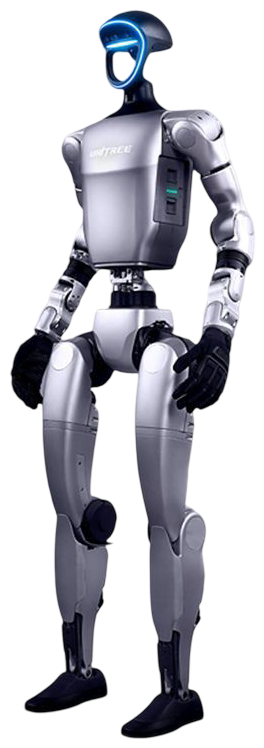
\includegraphics[width=\linewidth]{G1.jpeg}}{%
  \IfFileExists{Images/G1.jpg}{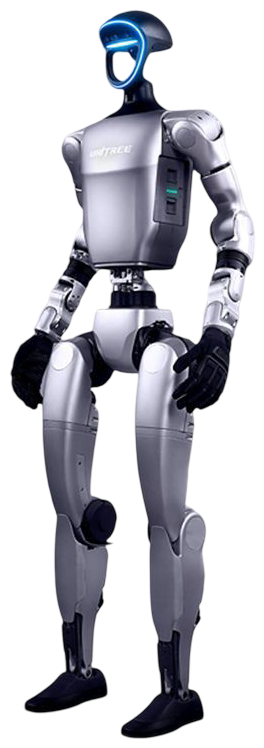
\includegraphics[width=\linewidth]{G1.jpg}}{%
  \IfFileExists{Images/G1.png}{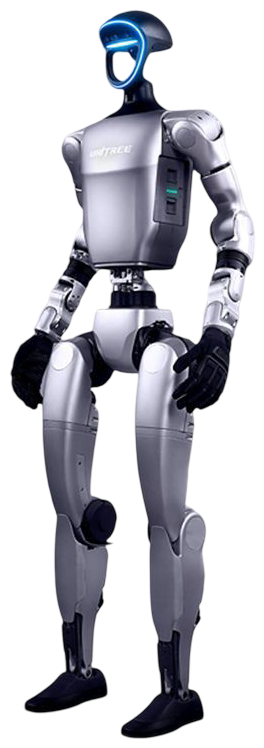
\includegraphics[width=\linewidth]{G1.png}}{%
    \fbox{\parbox[c][0.745\linewidth][c]{0.955\linewidth}{\centering\footnotesize\itshape
      photograph of the G1 humanoid\\[2pt] \textrm{(add \texttt{Images/G1.jpeg})}}}}}}}

\input{Configuration_files/config}

% --- metriche: macro e tabelle, generate dal repo del codice ----------------
\input{Metrics/metrics_macros}
\renewcommand{\restabdir}{Metrics/tab}

% Queste quattro metriche non sono (ancora) emesse da Metrics/metrics_macros.tex,
% che non e' versionato: senza definizione pdflatex esce con codice 1 e la frase
% resta muta. Segnaposto visibili, da sostituire con i valori misurati.
\providecommand{\resTermAbsMin}{\textbf{??}}
\providecommand{\resTermAbsMax}{\textbf{??}}
\providecommand{\resTermJMin}{\textbf{??}}
\providecommand{\resTermJMax}{\textbf{??}}

\renewcommand{\title}{Numerical Optimization for Map-Free Navigation:\\[2pt]
  Rolling-Horizon $A^\star$ and Nonlinear MPC on a Bipedal Humanoid}
\newcommand{\course}{062047 -- Numerical Optimization for Control}
\newcommand{\advisor}{Prof. Lorenzo Mario Fagiano}
% NOTE: le due matricole marcate 10... vanno completate.
\newcommand{\groupmembers}{Mateo Gomez - 10... \\ Lorenzo Ortolani - 10... \\ Francesco Pedrini - 10787879}
\newcommand{\YEAR}{2025-2026}
\newcommand{\keywords}{Nonlinear Model Predictive Control, Interior-Point Optimization, Exact Penalty Methods, Algorithmic Differentiation, Rolling-Horizon Planning, Legged Robot Navigation}
\renewcommand{\abstract}{Navigating an unknown environment without a prior map can be posed as two
optimization programs solved at every control cycle: a discrete shortest-path problem on an occupancy grid
rebuilt from the current LiDAR scan, and a continuous nonlinear program that turns the resulting geometric
reference into a body-frame velocity command subject to the actual kinematics, the actual input limits and a
clearance requirement. This report analyses that pair as optimization problems rather than as a robotics
pipeline. The program deployed on a Unitree~G1 humanoid is stated in full, its structure measured
($\resNvar$ decision variables, a $\resJacDensity\%$ dense constraint Jacobian), and every design decision it
embodies tested against the alternative the theory offers: mid-point against Euler integration, algorithmic
against numerical differentiation, exact against quasi-Newton Hessians, interior-point against active-set
solvers, sparse against condensed parametrisations, a smooth penalty against an exact $\ell^1$ relaxation of
the clearance constraint, a time-parametrised against a path-parametrised reference, and a terminal
equilibrium constraint against none. The first- and second-order optimality conditions are verified on
recorded missions rather than assumed. Several of the measurements contradict the design: the deployed
horizon is dominated on every objective, the integrator that is $\resIntegratorGain\times$ more accurate
buys nothing in closed loop, and the constraint that decides the outcome is not the one the cost was tuned
around. Every number in this document is generated from the deployed code by a single command and enters the
text through macros, so the report cannot silently diverge from the software it describes.}

\begin{document}

\input{Configuration_files/title_page_report}

\tableofcontents
\vspace{10pt}

%=============================================================================
\section*{Acronyms}
\addcontentsline{toc}{section}{Acronyms and notation}

\noindent\begin{tabularx}{\textwidth}{@{}lX@{\hspace{1.2em}}lX@{}}
AD    & algorithmic differentiation      & LTI   & linear time-invariant \\
AMO   & Adaptive Motion Optimization     & MPC   & model predictive control \\
DARE  & discrete algebraic Riccati equation & NLP & nonlinear program \\
FHOCP & finite-horizon optimal control problem & PD & proportional--derivative \\
IK    & inverse kinematics               & PPO   & proximal policy optimization \\
IMU   & inertial measurement unit        & QP    & quadratic program \\
KKT   & Karush--Kuhn--Tucker             & RL    & reinforcement learning \\
LICQ  & linear independence constraint qualification & ROS & Robot Operating System \\
LiDAR & light detection and ranging      & SQP   & sequential quadratic programming \\
\end{tabularx}

\section*{Notation}

\noindent All physical quantities carry SI units. Vectors are columns; $\|\cdot\|$ without
subscript is the Euclidean norm. Subscript $k$ indexes a node inside the prediction horizon,
subscript $j$ an obstacle. The symbol $\lambda_{\min}(\cdot)$ denotes the smallest eigenvalue of its
argument, and is not related to the multipliers $\lambda$.

\vspace{4pt}
\noindent\begin{tabularx}{\textwidth}{@{}lX@{\hspace{1.0em}}lX@{}}
\multicolumn{4}{@{}l}{\textit{State, input and model}}\\[2pt]
$x$ & state, Eq.~\eqref{eq:state}   & $\tau_v,\tau_w$ & actuator time constants [s] \\
$u$ & commanded body twist          & $\nu_v,\nu_w$ & discrete lag coefficients, Eq.~\eqref{eq:veldisc} \\
$p_x,p_y,\psi$ & world-frame pose [m], [rad] & $\Delta t$ & sampling time [s] \\
$v_x,v_y,\omega$ & body twist [m/s], [rad/s] & $N$ & prediction horizon [steps] \\
$t$ & continuous time [s]           & $\Ninput$ & control horizon [steps] \\[4pt]

\multicolumn{4}{@{}l}{\textit{Environment and reference}}\\[2pt]
$\mathcal{P}_k$ & LiDAR point cloud at cycle $k$ & $\delta$ & occupancy grid resolution [m] \\
$P(c)$ & occupancy of cell $c$      & $\sigma$ & Gaussian inflation width [m] \\
$x_g$ & goal position [m]           & $\theta$ & path abscissa, Sec.~\ref{sec:pathfollow} \\
$v_{\mathrm{ref}}$ & cruise speed [m/s] & $\pi_k$ & \astar{} path at cycle $k$ \\[4pt]

\multicolumn{4}{@{}l}{\textit{Optimization program}}\\[2pt]
$z=(X,U)$ & decision variables      & $\lambda,\mu$ & KKT multipliers (eq., ineq.) \\
$J$ & objective, Eq.~\eqref{eq:cost} & $\mu_b$ & interior-point barrier parameter \\
$Q,R,\Rjerk$ & tracking, effort, rate weights & $\rho_T$ & terminal weight multiplier \\
$\Wobs,\aobs,\robs$ & obstacle penalty height, steepness, radius & $\rho_s$ & slack penalty weight \\
$\dsafe$ & imposed clearance [m]    & $s_{jk}$ & constraint slack [m] \\
$\gamma(k)$ & robust back-off [m], Sec.~\ref{sec:robust} & $\kappa_j$ & scalarisation weights, Eq.~\eqref{eq:scalar} \\
$\varepsilon_d$ & distance regulariser & $\varepsilon_M$ & machine epsilon \\[4pt]

\multicolumn{4}{@{}l}{\textit{Locomotion layer (Sec.~\ref{sec:lowlevel})}}\\[2pt]
$q,\dot q$ & joint positions, velocities & $\beta$ & gait duty factor \\
$\mathcal{T}$ & joint torques        & $\zeta_i$ & stride phase of leg $i$ \\
$K_P,K_D$ & joint PD gains          & $\Tstr,\Tst,\Tsw$ & stride, stance, swing durations [s] \\
$\pf_i$ & foot position of leg $i$ [m] & $L_i$ & step length of leg $i$ [m] \\
\end{tabularx}

\vspace{6pt}

%=============================================================================
\section{Introduction}
\label{sec:intro}

A mobile robot that must reach a goal in an environment it has never seen has no global map to plan on: at
every instant it knows only what its sensors reported in the last few metres. The classical answer is to
decouple the problem into a geometric planner and a low-level tracker, but if the two layers ignore each
other the planner produces paths the actuators cannot execute, and the tracker produces commands the geometry
does not allow. Model Predictive Control (MPC) resolves the conflict by construction: it optimizes a finite
sequence of future inputs subject to the actual dynamics and the actual constraints, and re-optimizes at every
cycle \cite{rawlings2017mpc}. The price is computational for the motion planner point of view: a nonlinear program must be solved to sufficient
accuracy inside the sampling period, every period, on the robot. However, this rolling horizon path planning, allows the robot to avoid simultaneously localize and map the enviroment. The presence of only a localization module throguh an EKF and the lack of complete SLAM, enables less computationally expensive navigation stack, which is an important contribution of this report.

The goal is to analyze legged robotics navigation stack, such as a Unitree Go2 dog robot or a Unitree G1 humanoid robot. The stack is deployed and tested entirely on the G1 robot and previously developed on a Unitree Go2
quadruped, whose locomotion layer, the CHAMP gait controller \cite{champ} on the simulated robot, the
vendor's sport-mode controller on the physical one, exposes a body-frame velocity interface; the same code
has since been ported to a Unitree G1 humanoid walking under a reinforcement-learning locomotion policy
\cite{li2025amo}, which is what makes the ``robot-agnostic'' claim testable, due to the simple high level
holonomic kinematic model derived from both systems. Section~\ref{sec:lowlevel} describes those two
locomotion layers and the abstraction that makes them interchangeable. Two programs are
solved at every planning cycle and are the object of the analysis:

\begin{itemize}
  \item a \emph{discrete} shortest-path program --- an \astar{} search over a Gaussian occupancy grid rebuilt
        from the current LiDAR scan, whose solution is a geometric reference and whose rolling-horizon target
        is the intersection of the ray to the global goal with the grid boundary;
  \item a \emph{continuous} nonlinear program --- a six-state, three-input MPC with actuator-lag dynamics, a
        smooth obstacle barrier and box-constrained inputs, formulated once symbolically in CasADi
        \cite{andersson2019casadi} and solved by the interior-point method IPOPT
        \cite{wachter2006ipopt} at $10$~Hz.
\end{itemize}

On top of these two runtime programs sits a third, solved once offline: the \emph{black-box} program of
choosing the eleven cost weights of the MPC. Weight tuning is the practical bottleneck of any deployed MPC, since depending on the enviroment, MPC performance can vary significantly. The problem is that the closed-loop performance of the MPC is a gray-box function of unknown parameters, namely the weights for each cost term. The automatic weights tuning problem is
implemented with Gaussian-process surrogates \cite{rasmussen2006gp,shahriari2016bo} for finding the optimal weight vector $\hat\theta$ of the MPC cost function. 

% \paragraph{Contributions of this report.}
% \begin{enumerate}[label=(\roman*)]
%   \item A complete and self-contained statement of the three optimization problems as they are actually
%         implemented --- including the details that matter numerically and are usually left out of a system
%         paper: sentinel padding of the obstacle parameters to freeze the NLP sparsity pattern, the
%         non-negativity constraint on the forward velocity, the semi-definiteness of the stage weight, and
%         the exact zero-order-hold discretization of the lag dynamics (Sections~\ref{sec:problem}
%         and~\ref{sec:formulation}).
%   \item An analysis of the solver side: NLP dimensions, IPOPT configuration, warm starting, and the failure
%         handling that a hard real-time deployment requires (Section~\ref{sec:optproc}).
%   \item A weight-tuning procedure sized to the budget a rollout-priced objective allows: one one-dimensional
%         Gaussian process per weight, swept in order of influence with each optimum carried forward, under an
%         explicit significance floor. It costs $67$ closed-loop rollouts, and it returns not only a tuned
%         vector but eleven measured curves showing how much each weight is worth
%         (Sections~\ref{sec:bo} and~\ref{sec:ofat}).
%   \item A quantitative closed-loop study --- eleven parametric campaigns, all driving the \emph{production}
%         CasADi/IPOPT tracker rather than a re-implementation --- of horizon length, sampling time, barrier
%         shape, effort and rate penalties, barrier count, terminal weight, warm start and model mismatch,
%         together with an ablation that identifies which weight group actually explains the tuning gain
%         (Section~\ref{sec:performance}).
%   \item A comparison of the deployed heuristic terminal cost with the infinite-horizon cost-to-go obtained
%         from the discrete algebraic Riccati equation of the linearised cruise dynamics
%         (Section~\ref{sec:terminal}), and an honest account of what the formulation does \emph{not}
%         guarantee (Section~\ref{sec:discussion}).
% \end{enumerate}

% The remainder of the report follows the natural order of the design. Section~\ref{sec:problem} analyses the
% system and derives the state-space model. Section~\ref{sec:formulation} formulates the two runtime
% optimization programs. Section~\ref{sec:optproc} describes the numerical solution procedure, including the
% offline Bayesian tuning of the cost weights. Section~\ref{sec:performance} reports the numerical results, and
% Sections~\ref{sec:discussion} and~\ref{sec:conclusions} discuss limitations and conclude.

%=============================================================================
\section{Problem analysis}
\label{sec:problem}

\subsection{System overview}
\label{sec:overview}

The stack is a chain of ROS~2 nodes that closes the loop between a 3-D LiDAR and the
body-frame velocity interface of the locomotion controller:

\begin{enumerate}[label=\arabic*.]
  \item an \textbf{odometry bridge} that converts the extended-Kalman-filter (EKF) pose estimate into a
        single pose topic and differentiates it, with an exponential filter, into a body-frame velocity estimate (the robot does
        not publish a usable body-frame twist);
  \item a \textbf{mapping module} that rebuilds a local Gaussian occupancy grid from the newest scan at
        $1$~Hz and maintains a sparse world-frame cell map of confirmed obstacle cells, on which the memory-augmented target rule of Section~\ref{sec:memoryfix} plans; its purpose
        is precisely to repair the failure mode analysed in Section~\ref{sec:localmin};
  \item the \textbf{\astar{} local planner}, which solves the discrete program of
        Section~\ref{sec:astar} on that grid;
  \item the \textbf{nonlinear MPC tracker}, which solves the NLP of Section~\ref{sec:nlp} at $10$~Hz and
        publishes a setpoint;
\end{enumerate}

% \begin{figure}[htbp]
%   \centering
%   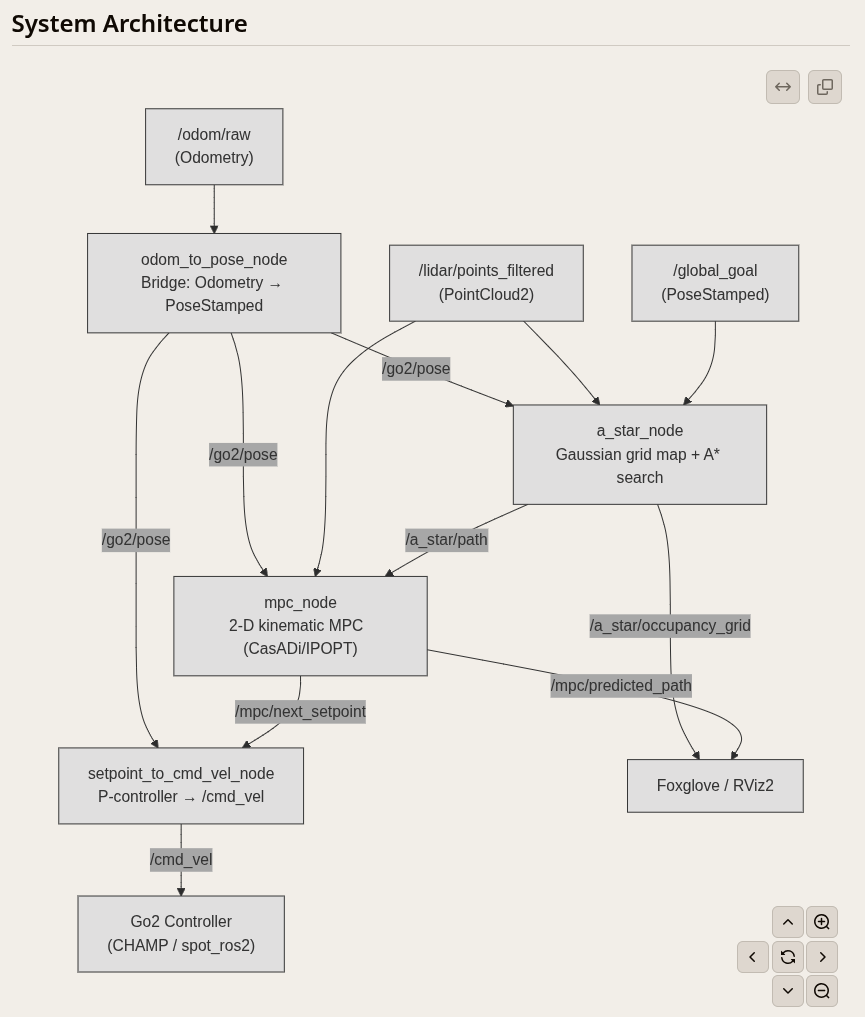
\includegraphics[width=0.86\textwidth]{system_architecture.png}
%   \caption{Architecture of the navigation stack. The two runtime optimization programs analysed in this
%   report are the \astar{} search on the Gaussian occupancy grid and the nonlinear MPC tracker; the Bayesian
%   tuning stage is executed offline and only produces the weight vector $\hat\theta$.}
%   \label{fig:arch}
% \end{figure}

Two design decisions shape everything that follows. First, the locomotion layer is treated as an ideal
velocity-tracking device with a time constant: we never model legs, contacts or gait, and the robot
is abstracted as a planar holonomic agent, Sections~\ref{sec:platforms} and~\ref{sec:lowlevel} describe
what that layer actually does on each of the two platforms, and why the same abstraction survives the
difference between them. Second, the map is \emph{local and volatile}. The
occupancy grid covers a fixed $10\times10$~m window centred on the robot and is rebuilt from scratch at every
planning cycle, so the planning problem is genuinely map-free, and the geometric reference the MPC tracks is
only valid for one grid width ahead. Section~\ref{sec:localmin} measures what this choice costs, and
Section~\ref{sec:memoryfix} what it takes to repair it.

\subsection{The controlled platforms}
\label{sec:platforms}

The same stack drives two robots whose mechanics could hardly be more different: a Unitree Go2 quadruped
(Fig.~\ref{fig:platforms}\subref{fig:platform-go2}) and a Unitree G1 humanoid
(Fig.~\ref{fig:platforms}\subref{fig:platform-g1}). The Go2 has
twelve actuated joints, three per leg; the G1 has twenty-nine, of which the locomotion layer of
Section~\ref{sec:g1rl} drives fifteen, the twelve leg joints and the three waist joints, while the arms
are held at a fixed posture. Neither joint set is ever addressed by the high level trajectory tracking MPC controller. Both
platforms are commanded through the same channel, a body-frame twist
$u=(v_x^{\mathrm{cmd}},v_y^{\mathrm{cmd}},\omega^{\mathrm{cmd}})$, and both carry a 3-D LiDAR whose returns
are the only exteroceptive input of the stack.

\begin{figure}[htbp]
  \centering
  \subfloat[Unitree Go2 quadruped\label{fig:platform-go2}]{%
    \begin{minipage}{0.47\textwidth}\centering
      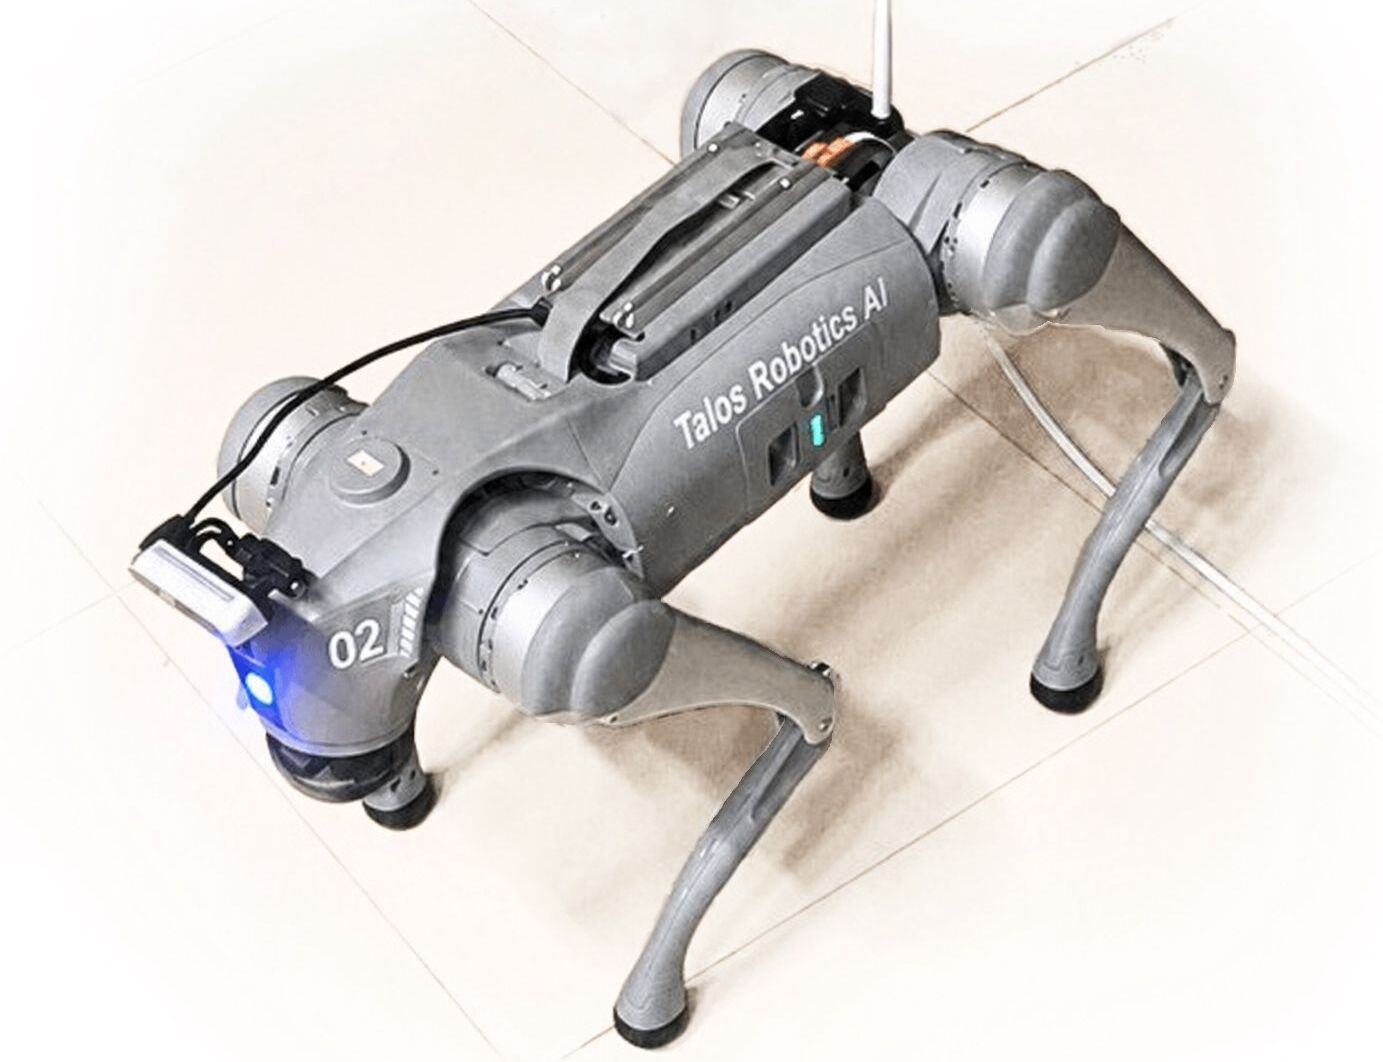
\includegraphics[width=\linewidth]{robot.jpeg}
    \end{minipage}}
  \hfill
  \subfloat[Unitree G1 humanoid\label{fig:platform-g1}]{%
    \begin{minipage}{0.47\textwidth}\centering
      \gonephoto
    \end{minipage}}
  \caption{The two platforms on which the same navigation stack is deployed. (a) The Go2 quadruped, with its LiDAR mounted on the head. (b) The G1
  humanoid, to which the stack was ported without changing the optimization program: only the constants of the
  actuator-lag model~\eqref{eq:lagcont} and the command mapping of Section~\ref{sec:g1rl} differ.}
  \label{fig:platforms}
\end{figure}

\begin{table}[htbp]
  \centering
  \small
  \caption{The two platforms as the controller sees them. The rows above the first rule are properties of the
  machine, those between the rules are properties of the locomotion layer that receives the MPC command, and
  those below are the ones that enter the optimization program: the prediction model~\eqref{eq:lagcont}, the
  admissible input set and the horizon. The two
  time constants were identified on the Go2 (Section~\ref{sec:model}) and carried over unchanged to the G1,
  which is the concrete form the ``robot-agnostic'' claim takes.}
  \label{tab:platforms}
  \begin{tabular}{lll}
    \toprule
                                  & Unitree Go2                     & Unitree G1 \\
    \midrule
    Morphology                    & quadruped                       & humanoid \\
    Actuated joints               & $12$ ($3$ per leg)              & $29$ ($15$ driven by the gait policy) \\
    Exteroception                 & Unitree L1 LiDAR                & Livox MID-360 LiDAR \\
    \midrule
    Locomotion layer              & CHAMP gait controller           & AMO reinforcement-learning policy \\
                                  & (vendor sport mode on hardware) & \\
    Layer update rate             & $200$~Hz                        & $50$~Hz \\
    Command interface             & body-frame twist $u$            & body-frame twist $u$, remapped \\
                                  &                                 & (Section~\ref{sec:g1rl}) \\
    \midrule
    Abstraction used by the MPC   & \multicolumn{2}{c}{first-order velocity lag, $\tau_v=0.12$~s, $\tau_w=0.10$~s} \\
    Admissible input set          & \multicolumn{2}{l}{$v_x\in[\resVxMin,\,\resVxMax]$~m/s, $|v_y|\le\resVyMax$~m/s, $|\omega|\le\resOmegaMax$~rad/s} \\
    Horizon                       & \multicolumn{2}{l}{$N=\resN$, $\Delta t=\resDt$~s ($\resHorizonSeconds$~s of preview), re-solved at $8$~Hz} \\
    \bottomrule
  \end{tabular}
\end{table}

\subsection{Low-level locomotion layers}
\label{sec:lowlevel}

The controller analysed in this report never commands a joint. Its decision variable is a body-frame twist,
and between that twist and the ground sits a platform-specific layer that turns it into joint commands at
$200$~Hz on the Go2 and $50$~Hz on the G1. Only two properties of that layer reach the optimization problem:
the twist is tracked with a first-order lag rather than instantaneously, and the tracking is fast enough,
relative to the $10$~Hz MPC cycle, for the two layers to be designed separately. This section describes the
two locomotion controllers to the depth needed to justify those two properties and no further. Throughout, $q\in\R^{n_j}$
denotes the vector of joint positions ($n_j=12$ on the Go2, $n_j=29$ on the G1), $\mathcal{T}\in\R^{n_j}$ the
vector of joint torques, and $K_P,K_D\succ0$ the diagonal proportional and derivative gain matrices of the
joint-level loop; the symbol $\tau$ is reserved for the actuator time constants of
Section~\ref{sec:model}.

\subsubsection{Model-based gait generation: CHAMP on the Go2}
\label{sec:champ}

CHAMP \cite{champ} is an open-source implementation of the hierarchical trot controller developed for the MIT
Cheetah \cite{lee2013hierarchical,hyun2014trot}. It is a purely feedforward pipeline: a pattern modulator
imposes the footfall sequence, a trajectory planner turns each leg's phase into a foot position, inverse
kinematics (IK) turns that position into joint angles, and a joint-level impedance loop tracks them. CHAMP is the locomotion layer of the simulated robot.

\paragraph{Pattern modulation.} Let $t$ denote time. Each leg $i\in\{\mathrm{LF},\mathrm{RF},\mathrm{LH},
\mathrm{RH}\}$ carries a normalised stride clock
\begin{equation}
  \zeta_i(t)=\left(\frac{t}{\Tstr}-\zeta_i^{0}\right)\bmod 1\in[0,1),
  \qquad \Tstr=\Tst+\Tsw ,
  \label{eq:gaitphase}
\end{equation}
where $\Tst$ and $\Tsw$ are the stance and swing durations and $\zeta_i^{0}$ is the phase offset of leg $i$.
Leg $i$ is in stance while $\zeta_i<\beta$ and in swing otherwise, with duty factor $\beta=\Tst/\Tstr$. The
deployed configuration uses $\Tst=\Tsw=0.25$~s, hence $\Tstr=0.5$~s and $\beta=0.5$, and
$\zeta^{0}=(0,\tfrac12,\tfrac12,0)$: the diagonal pairs move together, which is the trot.

\paragraph{Where the command enters.} The commanded twist does not act on the legs directly; it acts on the
\emph{step geometry}, through the Raibert foot-placement heuristic \cite{raibert1986legged}: a foot is placed
half a step ahead of its nominal position, so that sweeping backwards during the stance interval $\Tst$
displaces the trunk by exactly the commanded amount. Let $\bar\pf_i\in\R^3$ be the nominal (zero-command)
position of foot $i$ in the body frame. Translating the nominal stance by the half-step
$\tfrac{1}{2}\Tst\,(v_x^{\mathrm{cmd}},v_y^{\mathrm{cmd}},0)^{\!\top}$ and rotating it about the vertical axis
by the half-stance yaw $\chi_g$ gives the foot displacement
\begin{equation}
  \Delta\pf_i \;=\; R_z(\chi_g)\Big(\bar\pf_i+\tfrac{1}{2}\Tst\,
                  \big(v_x^{\mathrm{cmd}},v_y^{\mathrm{cmd}},0\big)^{\!\top}\Big)-\bar\pf_i ,
  \qquad
  \chi_g = 2\sin\!\Big(\tfrac{1}{4}\Tst\,\omega^{\mathrm{cmd}}\Big)\approx\tfrac{1}{2}\Tst\,\omega^{\mathrm{cmd}} ,
  \label{eq:raibert}
\end{equation}
with $R_z(\cdot)$ the elementary rotation about the vertical axis.\footnote{The implementation obtains
$\chi_g$ from the tangential half-step $\tfrac12\Tst\,\omega^{\mathrm{cmd}}d_c$, with $d_c$ the horizontal
distance from the trunk centre to the nominal foot; $d_c$ cancels, leaving~\eqref{eq:raibert}. The small-angle
form on the right is the yaw swept in half a stance interval, as expected.} The step length and the heading of
the foot trajectory of leg $i$ follow as
\begin{equation}
  L_i = 2\big\|\Delta\pf_i\big\|_2 ,
  \qquad
  \chi_i=\operatorname{atan2}\big(\Delta\pf_{i,y},\,\Delta\pf_{i,x}\big),
  \label{eq:steplen}
\end{equation}
the factor $2$ turning the half-step into the full stride of the foot. Equations~\eqref{eq:raibert} and
\eqref{eq:steplen} are the whole of the command path: the three numbers the MPC publishes are compressed into
one length and one angle per leg, and nothing else of the command reaches the robot.

\paragraph{Foot trajectories and impedance.} With phase and step length fixed, each foot follows a planar
curve in its own trajectory frame, rotated by $\chi_i$ and added to the nominal stance:
$\pf_i=\bar\pf_i+(\,\xi\cos\chi_i,\ \xi\sin\chi_i,\ \eta\,)^{\!\top}$, where $\xi$ and $\eta$ are the
longitudinal and vertical coordinates of the curve. In stance, parametrised by the normalised stance phase
$\zeta_i^{\mathrm{st}}=\zeta_i/\beta\in[0,1)$, the foot sweeps backwards along a shallow arc that presses into
the ground by $h_{\mathrm{st}}$,
\begin{equation}
  \xi=\tfrac{L_i}{2}\left(1-2\zeta_i^{\mathrm{st}}\right),\qquad
  \eta=-h_{\mathrm{st}}\cos\!\left(\frac{\pi\,\xi}{L_i}\right);
  \label{eq:stance}
\end{equation}
in swing, parametrised by $\zeta_i^{\mathrm{sw}}=(\zeta_i-\beta)/(1-\beta)\in[0,1)$, it follows a Bézier curve
of degree $11$ through twelve control points $b_j\in\R^2$,
\begin{equation}
  (\xi,\eta)=\sum_{j=0}^{11}\binom{11}{j}
             \big(\zeta_i^{\mathrm{sw}}\big)^{j}\big(1-\zeta_i^{\mathrm{sw}}\big)^{11-j}\,b_j ,
  \label{eq:swing}
\end{equation}
whose horizontal spread is scaled by $L_i$ and whose vertical spread is scaled by the swing height
$h_{\mathrm{sw}}$. Figure~\ref{fig:gaitparams} collects these quantities on a single leg. The deployed gait uses $h_{\mathrm{sw}}=0.04$~m, $h_{\mathrm{st}}=0.01$~m and a nominal
trunk height $h_0=0.225$~m. A closed-form IK then maps each foot position to the three joint angles of its
leg, $q_i^{\mathrm{ref}}=\mathrm{IK}_i(\pf_i)$, and a proportional--derivative (PD) law closes the loop at the
joints,
\begin{equation}
  \mathcal{T}_i = K_P\big(q_i^{\mathrm{ref}}-q_i\big)+K_D\big(\dot q_i^{\mathrm{ref}}-\dot q_i\big)
  \;=\;\bm{J}_i(q_i)^{\!\top}F_i ,
  \label{eq:impedance}
\end{equation}
where $\bm{J}_i$ is the foot Jacobian of leg $i$, set in bold to distinguish it from the MPC cost $J$ and
from the tuning objective $\mathcal{J}$ and $F_i$ the equivalent force at the
foot. The PD loop is in joint space and
realises a virtual spring--damper at the foot, of Cartesian stiffness
$\bm{J}_i^{-\top}K_P\bm{J}_i^{-1}$, so the leg absorbs terrain irregularity and impact by
programmable compliance rather than by contact sensing or force control. This is what makes an open-loop gait
generator survive on a real robot.

\begin{figure}[htbp]
  \centering
  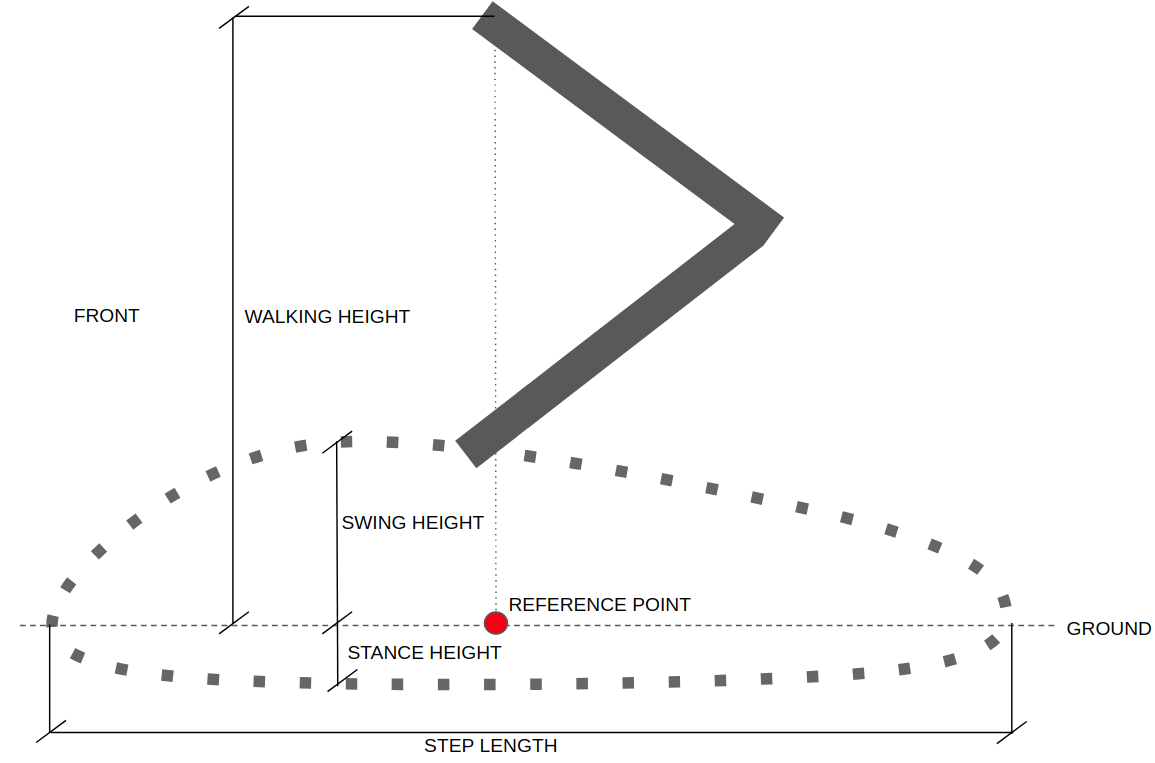
\includegraphics[width=0.72\textwidth]{gait_parameters.png}
  \caption{Geometry of the CHAMP gait on a single leg, seen from the side. The dotted closed curve is the
  cycle described by the foot in its trajectory frame: the upper branch is the swing
  Bézier~\eqref{eq:swing}, which clears the ground by the swing height $h_{\mathrm{sw}}$, and the lower branch
  is the stance arc~\eqref{eq:stance}, which presses into the ground by the stance height $h_{\mathrm{st}}$
  and sweeps backwards to carry the trunk forward. The horizontal extent of the cycle is the step length
  $L_i$ of~\eqref{eq:steplen}, the only channel through which the commanded twist reaches the leg; the
  reference point on the ground line is the nominal stance position $\bar\pf_i$ about which the Raibert
  half-step~\eqref{eq:raibert} displaces the cycle, and the walking height is the nominal trunk height $h_0$.
  Adapted from the CHAMP documentation \cite{champ}.}
  \label{fig:gaitparams}
\end{figure}

\paragraph{Low level joint controllers modelled as a lag.} Three consequences propagate upstream, and they are the reason
the model of Section~\ref{sec:model} has the form it has. First, the twist enters only through the step
geometry~\eqref{eq:steplen}: no measured trunk velocity is fed back, so the layer is a feedforward map and the
trunk velocity approaches the commanded one over roughly one stride rather than immediately. Second, that
step geometry is re-evaluated only once per stride, so a command that changes faster than $1/\Tstr=2$~Hz is
averaged, not tracked; a first-order lag with $\tau_v=0.12$~s reaches $98\%$ of its final value in
$4\tau_v\approx\Tstr$, which is why the one-parameter fit of Section~\ref{sec:model} describes the layer as
well as it does. Third, the gait applies its own saturation, $|v_x^{\mathrm{cmd}}|\le0.3$~m/s,
$|v_y^{\mathrm{cmd}}|\le0.25$~m/s and $|\omega^{\mathrm{cmd}}|\le0.5$~rad/s in the deployed configuration.

\subsubsection{Learned whole-body control: the AMO policy on the G1}
\label{sec:g1rl}

On the humanoid the same interface is produced by a neural network instead of a gait generator. The deployed
controller is AMO (Adaptive Motion Optimization) \cite{li2025amo}, a reinforcement-learning (RL) policy
trained in simulation for the G1 and its twenty-nine degrees of freedom (DoF). AMO is deliberately \emph{not} a walking controller: it is a
loco-manipulation policy, trained to track torso height, torso orientation and upper-body targets while
walking, on a hybrid dataset in which an offline trajectory-optimization module supplies whole-body
references that are kinematically consistent with the commanded end-effector motion. The navigation stack
exercises only its locomotion subset, the arms are held at the default posture and only the base command
is driven, but the policy is the one trained for the larger task, which is what makes the same platform
usable for manipulation later without changing the layer the MPC talks to.

\paragraph{Structure.} At each tick $k$ of the $50$~Hz policy loop, the network maps an observation to an
action,
\begin{equation}
  a_k=\pi(o_k)\in\R^{15},
  \qquad
  o_k=\big(\,\omega^{\mathrm{b}}_k,\ \hat g_k,\ \tilde u_k,\ q_k-\qdef,\ \dot q_k,\ a_{k-1}\,\big),
  \label{eq:rlpolicy}
\end{equation}
where $\omega^{\mathrm{b}}_k\in\R^3$ is the body angular velocity, $\hat g_k\in\R^3$ the gravity direction
expressed in the body frame (the tilt an inertial measurement unit (IMU) provides without a global heading), $q_k,\dot q_k$ the
measured joint positions and velocities of the $23$ observed joints, $\qdef$ the default posture,
$a_{k-1}$ the previous action, and $\tilde u_k$ the command. The action is not a torque: it is an offset on
the default posture, which the same joint-level PD law as~\eqref{eq:impedance} converts into torque,
\begin{equation}
  q_k^{\mathrm{ref}}=\qdef+s_a\,a_k,
  \qquad
  \mathcal{T}_k=K_P\big(q_k^{\mathrm{ref}}-q_k\big)+K_D\big(0-\dot q_k\big),
  \label{eq:rlpd}
\end{equation}
with $s_a$ a fixed action scale and a zero reference joint velocity. The learned part of the controller is
therefore exactly the map from observation to PD setpoint; the stabilising loop underneath it is the same
fixed impedance as on the quadruped. The policy $\pi$ is obtained by proximal policy optimization (PPO)
\cite{schulman2017ppo}, maximising the expected discounted return
$\mathbb{E}\big[\sum_k\gamma^k\mathcal{R}_k\big]$ with $\gamma\in(0,1)$ and a stage reward $\mathcal{R}_k$
that pays for tracking the commanded twist and penalises posture deviation, joint effort and action rate;
masses, friction, gains and latencies are randomised during training so that the fixed policy transfers to
hardware \cite{rudin2022walk}.

% \paragraph{The command mapping.} The command handed to the network is not the MPC twist but its image under a
% calibrated map, $\tilde u_k=\mathcal{M}(u_k)$, and that map is not a change of units. The policy's yaw channel
% is a heading \emph{offset} saturating at $\pm0.2$~rad rather than a yaw rate, its lateral channel uses the
% opposite sign convention, and the policy plants its feet whenever all three channels fall below a stand gate
% of about $0.1$ of full scale. The constants of $\mathcal{M}$ were identified so that the achieved twist
% matches the commanded one to within $10\%$ over the operating range. The stand gate is the one visible
% unmodelled nonlinearity of the cascade: a near-pure rotation in place, which the MPC produces when the
% reference turns sharply at low speed, falls below it and returns no motion at all.

\subsubsection{The cascade and its abstraction seam}
\label{sec:cascade}

Fig.~\ref{fig:cascade} places the two locomotion layers in the control structure they belong to. The stack is
a cascade of four loops whose rates are separated by roughly a decade each: the \astar{} reference is
recomputed at $1$~Hz, the MPC at $10$~Hz, the locomotion layer at $50$--$200$~Hz, and the joint PD loop at the
motor-driver rate. That separation is the standard justification for designing each layer against a static
abstraction of the one below it, and the abstraction used here is deliberately minimal: three decoupled
first-order lags, Eq.~\eqref{eq:lagcont}, whose time constants are identified in Section~\ref{sec:model}. Both
locomotion layers, the hand-designed one and the learned one, are approximated by the same two numbers.

% This is the entire content of the ``robot-agnostic'' claim, and it is worth stating what it costs. The
% abstraction discards leg dynamics, contact, footstep timing and the two nonlinearities named above --- the
% gait saturation of Section~\ref{sec:champ} and the stand gate of Section~\ref{sec:g1rl}. What survives is a
% question of degree rather than of principle, and Section~\ref{sec:mismatch} answers it quantitatively by
% inflating the plant lags by $60$--$67\%$ against the model and measuring what the closed loop loses.

\begin{figure}[htbp]
  \centering
  \begin{tikzpicture}[
    font=\footnotesize,
    >={Latex[length=1.8mm]},
    blk/.style={draw, rounded corners=3pt, align=center, inner sep=5pt, minimum height=8mm,
                fill=black!3},
    hlblk/.style={draw=bluePoli, line width=0.9pt, rounded corners=3pt, align=center, inner sep=5pt,
                  minimum height=8mm, fill=bluePoli!10},
    sig/.style={->, semithick},
    sl/.style={font=\scriptsize, inner sep=2.2pt},
  ]
    % ------------------------------------------------------------------ planning
    \node[blk,  text width=46mm] (astar) at (0,6.1) {\astar{} search on the occupancy grid\\$1$~Hz};
    \node[hlblk,text width=46mm] (mpc)   at (0,4.1) {nonlinear MPC tracker\\$10$~Hz};

    \draw[sig] (0,7.15) -- node[sl,right] {goal $x_g$} (astar.north);
    \draw[sig] (astar) -- node[sl,right] {$x^{\mathrm{ref}}$} (mpc);

    % --------------------------------------------------------- locomotion layer
    \coordinate (split) at (0,2.3);
    \node[blk, text width=52mm] (champ) at (-3.8,0.75)
      {\textbf{Go2}: CHAMP gait generator\\
       phase~\eqref{eq:gaitphase} $\to$ step~\eqref{eq:steplen} $\to$ foot~\eqref{eq:swing}\\
       $\to$ IK $\to$ joint PD, $200$~Hz};
    \node[blk, text width=52mm] (rl) at (3.8,0.75)
      {\textbf{G1}: AMO reinforcement-learning policy\\
       $\mathcal{M}\to\pi$~\eqref{eq:rlpolicy} $\to$ PD setpoint~\eqref{eq:rlpd}\\
       $\to$ joint PD, $50$~Hz};
    \node[draw, dashed, rounded corners=4pt, fit=(champ)(rl), inner sep=7pt] (llbox) {};
    \node[sl, anchor=south west] at ([xshift=2pt,yshift=1.5pt]llbox.north west)
      {low-level locomotion layer};

    \draw[sig] (mpc.south) -- node[sl, right, align=left, xshift=1pt]
      {$u=(v_x,v_y,\omega)^{\mathrm{cmd}}$\\ first-order lag~\eqref{eq:lagcont}} (split);
    \draw[sig] (split) -| ([xshift=12mm]champ.north);
    \draw[sig] (split) -| ([xshift=-12mm]rl.north);

    % ------------------------------------------------------------------- plant
    \node[blk, text width=28mm] (robot) at (0,-2.3) {robot $+$ ground};
    \draw[sig] ([xshift=12mm]champ.south) -- (robot.north west);
    \draw[sig] ([xshift=-12mm]rl.south)   -- (robot.north east);
    \node[sl] at (0,-1.35) {$\mathcal{T}$: joint torques};

    % ---------------------------------------------------------------- feedback
    \node[blk, text width=38mm] (est)  at (6.2,4.1) {state estimation (EKF)\\$\hat x$: pose $+$ body twist};
    \node[blk, text width=38mm] (grid) at (6.2,6.1) {Gaussian occupancy grid\\$\mathcal{P}_k$, rebuilt at $1$~Hz};

    \draw[semithick] (robot.east) -- node[sl, above] {LiDAR, IMU, encoders} (9.2,-2.3) -- (9.2,6.1);
    \draw[sig] (9.2,4.1) -- (est.east);
    \draw[sig] (9.2,6.1) -- (grid.east);
    \draw[sig] (est.west)  -- (mpc.east);
    \draw[sig] (grid.west) -- (astar.east);
  \end{tikzpicture}
  \caption{Cascaded structure of the controller, from the goal down to joint torques. The
  rates fall by roughly a decade at every seam ($1$~Hz, $10$~Hz, $50$--$200$~Hz, motor-driver rate), which is
  what allows the layers to be designed separately, and the two branches inside the dashed box, a
  hand-designed gait generator and a learned policy, are interchangeable precisely because they present the
  same twist interface $u$.}
  \label{fig:cascade}
\end{figure}

\subsection{Environment representation}
\label{sec:grid}

Let $\mathcal{P}_k=\{p_i\in\R^3\}_{i=1}^{N_k}$ be the LiDAR point cloud available at cycle $k$, projected on
the plane. The grid is a square of side $2h_w$ ($h_w=5$~m) centred on the robot position, discretised with
resolution $\Delta=0.25$~m into $n_c=2h_w/\Delta=40$ cells per axis. The occupancy probability of cell $c$ is
a Gaussian tail of the distance to the nearest return,
\begin{equation}
  P(c) \;=\; 1-\Phi\!\left(\frac{d_{\min}(c,\mathcal{P}_k)}{\sigma}\right),
  \qquad d_{\min}(c,\mathcal{P}_k)=\min_{p\in\mathcal{P}_k}\|c-p\|_2 ,
  \label{eq:grid}
\end{equation}
with $\Phi$ the standard normal cumulative distribution function,
\begin{equation}
  \Phi(x) \;=\; \frac{1}{\sqrt{2\pi}}\int_{-\infty}^{x}e^{-t^2/2}\,\mathrm{d}t
  \;=\; \frac{1}{2}\left(1+\operatorname{erf}\!\left(\frac{x}{\sqrt{2}}\right)\right)\in(0,1),
  \label{eq:phi}
\end{equation}
and $\sigma=0.15$~m. Equation~\eqref{eq:grid} is an \emph{inflation}
model: it is a smooth, monotone map from clearance to cost, whose one parameter $\sigma$ sets the width of
the obstacle halo. Cells with $P(c)\ge P_{\mathrm{thr}}=0.4$ are hard obstacles. The left panel of
Fig.~\ref{fig:occprofile} shows the trade-off governed by $\sigma$: a small $\sigma$ leaves doorways open but
hugs walls, a large one closes gaps the robot could physically cross.

Because the grid is rebuilt from scratch, its construction cost is the dominant cost of the planning layer,
$O(n_c^2\,|\mathcal{P}_k|)$; vectorised over $40\times40$ cells and ${\sim}180$ returns it measures
$4$--$5$~ms on average together with the \astar{} search (Section~\ref{sec:setup}), which at the $1$~Hz
replanning rate is negligible against the $10$~Hz MPC.

\begin{figure}[htbp]
  \centering
  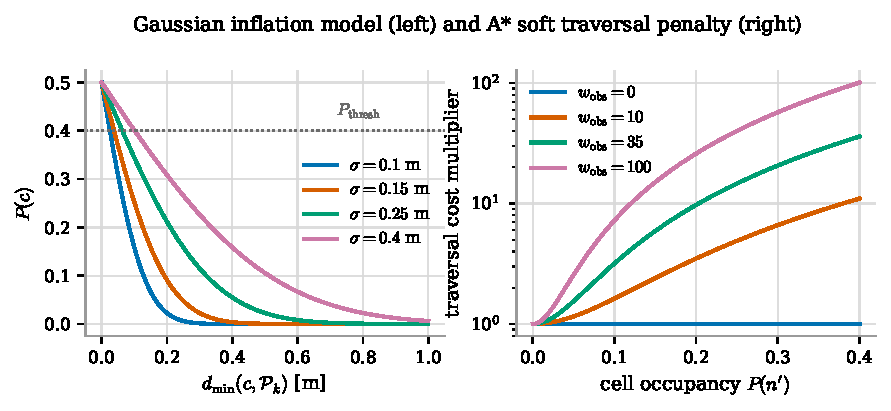
\includegraphics[width=0.92\textwidth]{fig_occupancy_profile.pdf}
  \caption{Left: the Gaussian inflation model~\eqref{eq:grid} for four values of $\sigma$, with the hard
  threshold $P_{\mathrm{thr}}=0.4$. Right: the soft traversal-cost multiplier
  $1+w_{\mathrm{obs}}(P/P_{\mathrm{thr}})^2$ of the \astar{} edge cost~\eqref{eq:astarcost}, which is what
  actually keeps the path away from walls; the deployed value is $w_{\mathrm{obs}}=35$.}
  \label{fig:occprofile}
\end{figure}

\subsection{Plant model and state-space formulation}
\label{sec:model}

The MPC model must predict where the robot will be. Commanding a legged platform
a body-frame velocity does not produce that velocity instantaneously: the locomotion controller responds with
a measured time constant of $\tau\approx0.10$--$0.15$~s, which over a $5$~s horizon accumulates into a
prediction error of several tens of centimetres if neglected. The model therefore augments the usual planar
kinematic state with the three velocity states, giving
\begin{equation}
  x \;=\; \begin{bmatrix} p_x & p_y & \psi & v_x & v_y & \omega\end{bmatrix}^{\!\top}\in\R^{6},
  \qquad
  u \;=\; \begin{bmatrix} v_x^{\mathrm{cmd}} & v_y^{\mathrm{cmd}} & \omega^{\mathrm{cmd}}\end{bmatrix}^{\!\top}\in\R^{3},
  \label{eq:state}
\end{equation}
where $(p_x,p_y)$ and $\psi$ are the world-frame pose and $(v_x,v_y,\omega)$ the body-frame twist actually
realised by the platform. In continuous time the actuator behaves as three decoupled first-order lags driven
by the commands,
\begin{equation}
  \dot v_x = \frac{u_1-v_x}{\tau_v},\qquad
  \dot v_y = \frac{u_2-v_y}{\tau_w},\qquad
  \dot \omega = \frac{u_3-\omega}{\tau_w},
  \label{eq:lagcont}
\end{equation}
while the pose obeys the holonomic body-to-world rotation
\begin{equation}
  \dot p_x = v_x\cos\psi - v_y\sin\psi,\qquad
  \dot p_y = v_x\sin\psi + v_y\cos\psi,\qquad
  \dot\psi = \omega .
  \label{eq:kincont}
\end{equation}
The identified constants are $\tau_v=0.12$~s and $\tau_w=0.10$~s.
% \footnote{In the deployed code the lateral
% velocity $v_y$ is propagated with $\tau_w$ rather than $\tau_v$, i.e.\ lateral motion is assumed to respond as
% fast as yaw. The two constants differ by $20$~ms, well inside the identification uncertainty, so the
% substitution is numerically immaterial; it is reported here because the analysis reproduces the deployed
% formulation exactly rather than an idealisation of it.}

Model~\eqref{eq:lagcont}--\eqref{eq:kincont} is holonomic: unlike a differential-drive vehicle, the platform
can command a lateral velocity, so no nonholonomic constraint appears and the input set is a box. This is what
makes the resulting NLP comparatively benign, the nonlinearity is confined to the rotation
$R(\psi)$ and to the obstacle distances.

% At the identified $\tau_v=0.12$~s the instantaneous model mispredicts the horizon
% end-point by ${\sim}7$~cm, which is of the same order as the tracking accuracy the controller is asked to
% deliver.

% \begin{figure}[htbp]
%   \centering
%   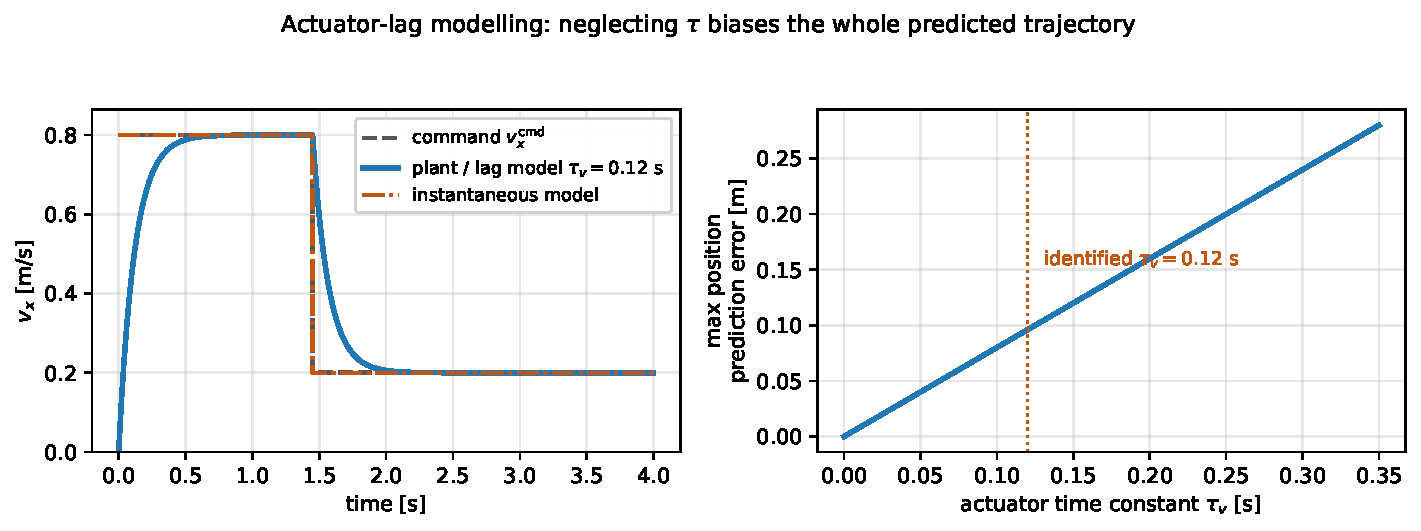
\includegraphics[width=0.92\textwidth]{fig_lag_model.pdf}
%   \caption{Actuator-lag modelling. Left: response of the first-order-lag model~\eqref{eq:lagcont} against the
%   instantaneous model $v\equiv u$ for a step in commanded forward velocity. Right: maximum position
%   prediction error accumulated over one $5$~s horizon by neglecting the lag, as a function of $\tau_v$.}
%   \label{fig:lag}
% \end{figure}

\subsection{Navigation problem statement}
\label{sec:statement}

Let $x_g\in\R^2$ be the goal. The navigation task is the receding-horizon optimal control problem
\begin{subequations}
\label{eq:ocp}
\begin{align}
  \min_{u_0,\dots,u_{N-1}}\;\; & J\!\left(x_{0:N},u_{0:N-1},\mathcal{P}_k,\theta\right) \label{eq:ocp-cost}\\
  \text{s.t.}\quad & x_{t+1}=f(x_t,u_t), && t=0,\dots,N-1, \label{eq:ocp-dyn}\\
                   & x_0 = \hat x(t_k), \label{eq:ocp-init}\\
                   & u_t\in\mathcal{U}, && t=0,\dots,N-1, \label{eq:ocp-input}\\
                   & d\!\left(x_t,\mathcal{P}_k\right)\ge r_{\min}, && t=0,\dots,N, \label{eq:ocp-obs}
\end{align}
\end{subequations}
solved at every control instant $t_k$. Two properties of the way~\eqref{eq:ocp} meets the robot are worth
stating before the design is read, because both are deviations from the textbook receding-horizon
implementation.

\emph{The sampling time of the model is not the period of the loop.} The step $\Delta t$
in~\eqref{eq:ocp-dyn} is the \emph{prediction} step, $0.35$~s in the deployed profile, while the program
itself is re-solved at $8$~Hz. The horizon is therefore re-planned about $2.8$ times per predicted node, and
the first predicted node already lies $0.35$~s of open loop ahead of the state that produced it. The two
quantities are independent design variables and are treated as such throughout.

\emph{Only $u_0$ would be applied --- but it is not.} The tracker does not publish $u^\star_0$. It walks the
predicted trajectory $x^\star_{0:N}$ out to a fixed look-ahead distance and publishes the point it reaches as
a geometric setpoint; a proportional law downstream converts that setpoint into the body twist actually sent
to the locomotion layer, at $20$~Hz. The optimizer is thus used as a \emph{reference generator} rather than
as a controller, and the loop closed on the robot is the cascade of that law with the locomotion policy
rather than~\eqref{eq:ocp} itself. Section~\ref{sec:setup} bypasses the stage deliberately, so that the
numerical results measure the optimization layer and not the tuning of the law beneath it.

Three features of~\eqref{eq:ocp} then determine the whole design:

\begin{itemize}
  \item \textbf{The goal is not reachable within the horizon.} With $N\Delta t=\resHorizonSeconds$~s and a
        cruise speed of $\resVref$~m/s the horizon spans about a metre and a half, while the goal may be tens of metres away
        and outside the sensed region altogether. The cost~\eqref{eq:ocp-cost} therefore cannot be a distance to $x_g$; it
        must be a distance to a \emph{reference trajectory} produced by a separate, cheaper program that
        looks further ahead. That program is the \astar{} search of Section~\ref{sec:astar}.
  \item \textbf{The obstacle set is a point cloud, not a polytope.} Constraint~\eqref{eq:ocp-obs} is
        non-convex, and its description changes at every cycle. It is relaxed into a smooth penalty
        (Section~\ref{sec:barrier}), which keeps the NLP smooth and always feasible at the price of losing
        the hard safety guarantee.
  \item \textbf{The cost is parametrised by $\theta$.} The eleven weights in $\theta$ are not physical
        quantities; they are design variables of a second-level optimization problem
        (Section~\ref{sec:bo}).
\end{itemize}

%=============================================================================
\section{Formulation of the optimization program}
\label{sec:formulation}

\subsection{Reference generation: \texorpdfstring{\astar{}}{A*} as a discrete program}
\label{sec:astar}

Section~\ref{sec:statement} established that the goal lies far outside the horizon, so the cost
of~\eqref{eq:ocp-cost} must measure the distance to a reference trajectory rather than to $x_g$. That
reference is produced once per replanning cycle by a discrete search on the occupancy grid of
Section~\ref{sec:grid}. Cells above the occupancy threshold are removed from the graph; the remaining
$8$-connected edges carry the cost
\begin{equation}
  g(n\rightarrow n') \;=\; c_{\mathrm{move}}\cdot\delta\cdot
  \left[1+w_{\mathrm{obs}}\left(\frac{P(n')}{P_{\mathrm{thr}}}\right)^{\!2}\right],
  \qquad c_{\mathrm{move}}\in\{1,\sqrt2\},
  \label{eq:astarcost}
\end{equation}
and a standard \astar{} search returns the cheapest path between two cells. The normalised quadratic
in~\eqref{eq:astarcost} is what produces medial-axis-like paths: a cell just below the hard threshold costs
($1+w_{\mathrm{obs}}$) times an open cell, so the search prefers the middle of a corridor to a shorter path
that grazes a wall, while a doorway is never closed outright. The Euclidean heuristic is admissible because
the bracket is bounded below by $1$, so no edge can be cheaper than its Euclidean length; the search is
therefore an exact \astar{} and returns a cost-optimal path on the current occupancy grid.

\paragraph{What the discrete layer is for.} Choosing \emph{which side} of an obstacle to pass on is a discrete decision. Take a trajectory that passes on the left and one that passes on the right: turning the first into the second means moving it continuously through intermediate trajectories, and at least one of those must run through the obstacle. The feasible set is therefore disconnected, with one component per side, and a gradient-based solver stays in the component its initial guess falls into: it converges to the best trajectory on one side and never learns that the other side existed. Writing the choice into the NLP would require binary variables and turn it into a mixed-integer nonlinear program, whose solution time is not compatible with a control loop at 8~Hz. A graph search represents the same choice natively, and on a $60\times60$
grid it costs a few milliseconds. Delegating the decision to the A* algorithm is therefore what leaves the continuous program
smooth, with a box-shaped input set and no integer variables --- the structure that
Sections~\ref{sec:dims} and~\ref{sec:solver} exploit throughout.

The price to pay for such delegation is that the choice is made before the MPC is consulted and the MPC has no way to
revise it: it can only deform the trajectory within the class it has been given. The two ways this breaks
are opposite to each other and both are measured in Section~\ref{sec:performance}. When the discrete layer
\emph{does not commit} --- an obstacle squarely on the line to the goal, two routes of equal cost --- the
smooth program inherits two competing basins of its own, and small perturbations flip the solution from one
to the other (Section~\ref{sec:bif}). When it \emph{commits on poor information}, the MPC follows it
faithfully into a dead end, because questioning the reference is not its job
(Section~\ref{sec:localmin}).

\paragraph{Choosing the target inside the window.} The search of~\eqref{eq:astarcost} runs on the local
grid, and the global goal is normally outside it, so a target on the window has to be selected first. This
is a selection over the free cells of the window boundary,
\begin{equation}
  x_{\mathrm{local}} \;=\;
  \operatorname*{arg\,min}_{c\,\in\,\partial\mathcal{W}(\hat x)\cap\mathcal{F}_k}
  \Big[\; d_k\big(c,\,x_g\big) \;+\; w_\tau\,\tau_k(c) \;\Big],
  \label{eq:localgoalargmin}
\end{equation}
where $\mathcal{F}_k$ are the free boundary cells, $d_k$ is a distance to the goal, and $\tau_k$ penalises
cells the robot has already visited without making progress. Only boundary cells are candidates, because
the boundary is where the direction of travel is decided; an interior cell would stop the robot half a
window short of the edge for no reason. The substantive choice in~\eqref{eq:localgoalargmin} is the metric
$d_k$. Two target rules were implemented and compared; only the second is an instance
of~\eqref{eq:localgoalargmin} at all, and that is itself part of the story.

The first, which the stack shipped with, does not solve~\eqref{eq:localgoalargmin} at all. It takes the
last free cell along the ray from the robot to the goal, which is a geometric shortcut rather than a
minimisation,
\begin{equation}
  x_{\mathrm{local}} \;=\;
  \begin{cases}
    \mathrm{cell}(x_g), & x_g\in\mathcal{W}(\hat x),\\[2pt]
    \mathrm{ray}(\hat x\!\rightarrow\! x_g)\cap\partial\,\mathcal{W}(\hat x), & \text{otherwise},
  \end{cases}
  \label{eq:localgoal}
\end{equation}
and the robot advances one grid width at a time towards the goal; if the projected cell is occupied, a
breadth-first search returns the nearest free one. The rule is cheap, needs no map at all, and is
memoryless and purely directional: whatever the map contains, the target lies on the line to the goal.
In front of a concave obstacle that line enters the concavity, so the target does too.

It would be convenient if the defect stopped there, because then~\eqref{eq:localgoalargmin} with a
Euclidean $d_k$ would already repair it. It does not. Figure~\ref{fig:localtarget} shows the robot at the
mouth of a horseshoe with the map it has actually observed: the ray projection selects a boundary cell
$\resFigProjGeo$~m of travel from the goal, and the $\arg\min$ of $\|c-x_g\|_2$ over the same free
boundary cells selects one $\resFigEuclGeo$~m away --- a different cell, and just as wrong. Both are near
the closed end, because in a straight line both are close to the goal. The straight-line distance rates a
cell inside the concavity and one outside it almost equally, and where the two happen to tie exactly it
separates them on numerical noise and reverses the choice at the next cycle.
Section~\ref{sec:localmin} shows that this is enough, on its own, to trap the robot.

The second instance is the deployed one. It keeps~\eqref{eq:localgoalargmin} and replaces $d_k$ with the
\emph{geodesic} distance to the goal over the free cells of the accumulated map: a wavefront propagated
from $x_g$, one scalar field per replanning cycle, with no path extracted from it. Space that has not been
observed yet counts as free. This is the optimistic assumption of frontier exploration, and it is what
makes the field correct itself as the sensor discovers: while the far end of a corridor is unseen the
wavefront runs through it and entering is the right decision, and as soon as that end is observed the same
cell becomes distant and the target is dropped. A candidate the wavefront cannot reach at all is discarded
rather than scored with a Euclidean fallback, which would readmit the metric at fault; if no candidate is
reachable on the known map the planner falls back to~\eqref{eq:localgoal}, which at least moves the robot
towards unknown ground. The memory term $w_\tau\tau_k$ is implemented but carries zero weight in the
deployed profile, for the reason measured in Section~\ref{sec:memoryfix}. In the same scene the geodesic
$\arg\min$ selects a cell $\resFigGeoGeo$~m from the goal, on the far side of the obstacle's arm, and
\astar{} routes out of the concavity instead of further into it.

\begin{figure}[htbp]
  \centering
  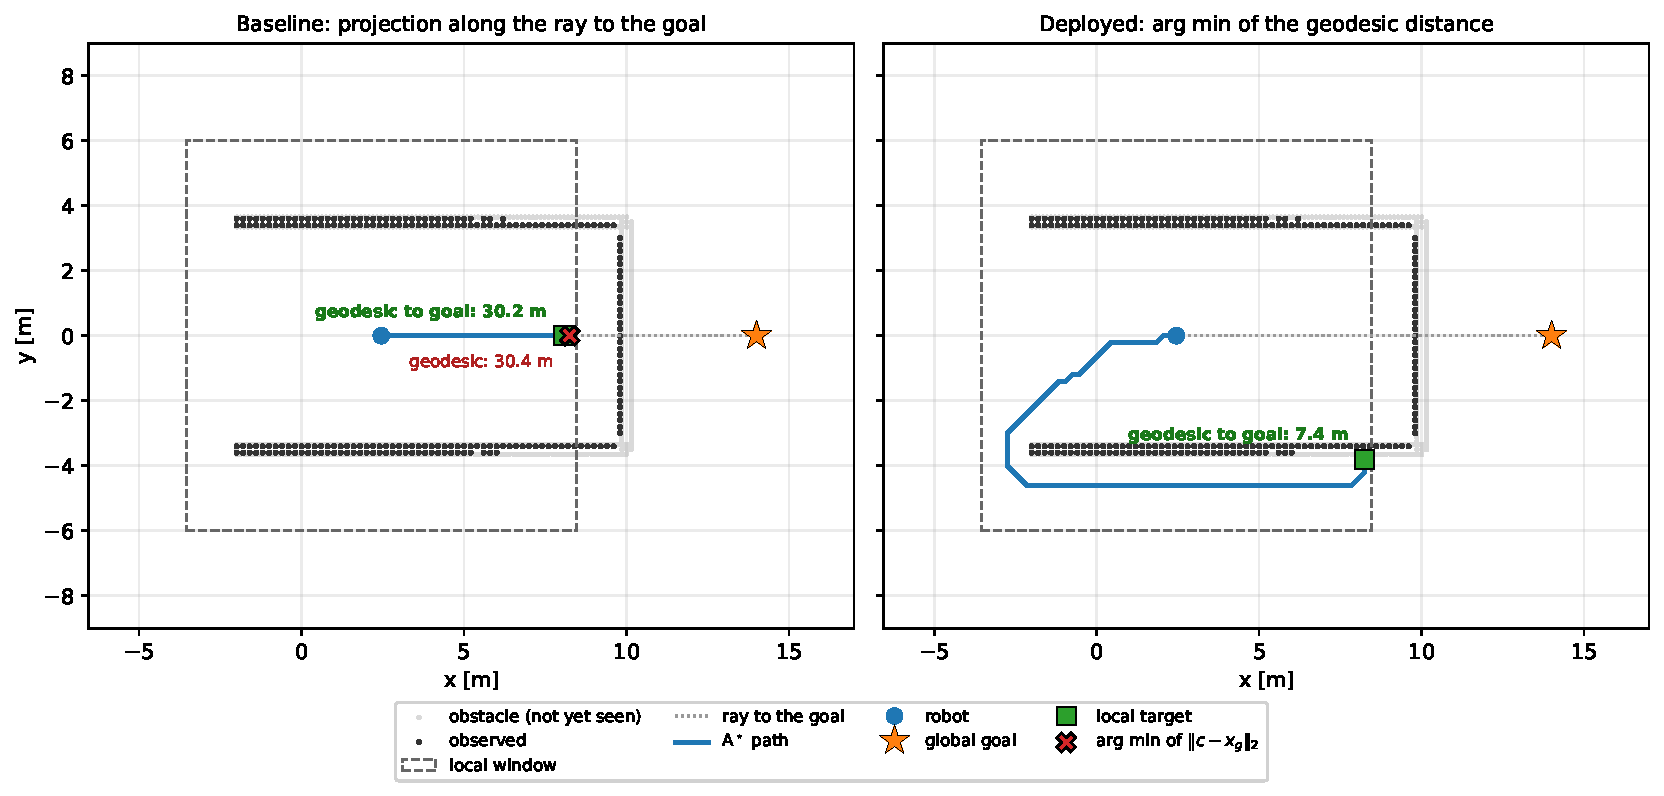
\includegraphics[width=\textwidth]{fig_local_target.pdf}
  \caption{The same scene, the same window and the same observed map; only the metric of
  \eqref{eq:localgoalargmin} changes. The robot sits at the mouth of a horseshoe and the map is the one it
  has actually accumulated by driving in, not the full world (light grey), which is what makes the failure
  reproducible. Left: the deployed projection~\eqref{eq:localgoal} puts the target at the closed end, and
  the $\arg\min$ of the Euclidean distance over the same free boundary cells lands beside it --- the two
  rules differ, the outcome does not, because both are $\sim\!30$~m of travel from the goal. Right: with the
  geodesic $d_k$ the target moves to the far side of the lower arm, $\resFigGeoGeo$~m away, and the
  \astar{} solution leaves the concavity. Drawn from the deployed planner and profile, not sketched.}
  \label{fig:localtarget}
\end{figure}

\paragraph{Commitment between replanning cycles.} Two boundary cells lying on opposite sides of an obstacle
can carry almost the same geodesic cost while belonging to different homotopy classes. The $\arg\min$ then
alternates between them from one cycle to the next, and the robot sways on the spot without ever
committing. The deployed rule therefore retains the candidate that best continues the previous choice
unless a competitor beats it by a margin of $2.0$~m of geodesic cost, and clears that memory whenever the
global goal changes, since a target inherited from a previous mission is simply the wrong direction. This
is the ambiguity of Section~\ref{sec:bif} seen one layer higher up: where the smooth program resolves it by
breaking symmetry numerically, the discrete layer resolves it by declining to switch without evidence.

The geodesic field is the one expensive part of the planning layer, because the wavefront covers the whole
known map rather than the window alone: it measures a median of $0.11$ to $0.15$~s per replanning cycle
depending on the world, with a worst case of $0.27$~s, which against the $1$~Hz replanning rate is between
a tenth and a quarter of the period and leaves the $8$~Hz MPC untouched. The resulting grid path is finally
resampled and smoothed with a moving average before it is handed to the MPC, to remove the zig-zag that the
$8$-connected discretisation introduces.

\subsection{Model discretization}
\label{sec:discretization}

With sampling time $\Delta t$, the lag subsystem~\eqref{eq:lagcont} is linear and time-invariant, so it is
discretised \emph{exactly} under a zero-order-hold input. Defining
$\nu_v = 1-e^{-\Delta t/\tau_v}$ and $\nu_w = 1-e^{-\Delta t/\tau_w}$, the velocity update is the
exact solution of~\eqref{eq:lagcont} over one step,
\begin{equation}
  v_{x,k+1}=(1-\nu_v)v_{x,k}+\nu_v u_{1,k},\qquad
  \omega_{k+1}=(1-\nu_w)\omega_{k}+\nu_w u_{3,k},
  \label{eq:veldisc}
\end{equation}
and analogously for $v_y$. No approximation is involved here and none should be claimed: this is the Lagrange
formula for a linear time-invariant (LTI) system under a piecewise-constant input, and it is exact at the sampling instants. On the
deployed G1 profile it is straightforward, since $\nu=1$ reduces~\eqref{eq:veldisc} to
$v_{k+1}=u_k$; the statement is retained because it is the part of the model that would carry the weight on hardware, where $\tau$ is real.

The pose, by contrast, is genuinely nonlinear and must be integrated numerically. Two possibilieties are implemented and compared:
\begin{align}
  \text{explicit Euler:}\quad & p_{k+1} = p_k + R(\psi_k)\,v_{k+1}\,\Delta t,
  \label{eq:euler}\\
  \text{mid-point (RK2):}\quad & p_{k+1} = p_k + R\!\left(\psi_k+\tfrac{1}{2}\omega_{k+1}\Delta t\right)v_{k+1}\,\Delta t.
  \label{eq:midpoint}
\end{align}
Both evaluate the rotation on the \emph{post-lag} velocity $v_{k+1}$, a semi-implicit choice that costs
nothing and removes the one-step delay that an explicit scheme would introduce between a command and the predicted
displacement. The mid-point rule differs from Euler by one addition inside the argument of the rotation.

The results shown in the following compare two integrators
outside the optimizer, which is only meaningful if the map assembled inside the NLP is the same one. That is
checked rather than assumed: a single transition is extracted from the CasADi program built by the tracker,
by reconstructing $f(x_0,u_0)$ from the first six equality constraints, and compared with the reference
implementation of~\eqref{eq:euler} and~\eqref{eq:midpoint}. The residual is zero to machine precision for both schemes.

\paragraph{Errors quantification according to the discretization method.} The global error of each scheme was first fitted against the step size
on three motion regimes, over a $\resOrderWindow$~s window, with the exact solution available in closed form:
at constant body velocity the pose traces a circular arc. The measured orders are $\resOrderEuler$ and
$\resOrderMidpoint$, exactly the first and second order the truncation analysis predicts, and the result is
identical across regimes. The step grid is built by halving from the deployed $\Delta t$, so the fit begins
at the step the controller actually uses rather than near it.

It is worth noting that a constant-velocity
arc is not the regime in which the MPC works. The optimizer applies a \emph{different} input at every node, and over a real horizon the commanded yaw rate changes sign.

The comparison is repeated on
$\resIntegBagCycles$ horizons taken from a bag of data recorded while G1 is navigating in a mapless MuJoCo world and re-solved with the deployed
profile, each integrated with its own optimal input sequence. The step is varied by subdividing the
prediction interval while the input stays constant over each $\Delta t$, which keeps an order measurable on a
real trajectory; the reference is the exact arc on the same post-lag velocity sequence, so the only
difference between the three trajectories is how $R(\psi)$ is evaluated.

\begin{table}[htbp]
  \centering
  \small
  \caption{%
  Median position error at the end of the horizon, over 12 horizons re-solved from a bag of data recorded during the navigation, against the exact arc on the same velocity sequence. The first row is the
  deployed step; the others subdivide the prediction interval without changing the input.}
  \label{res:tab:integbag}
  \restab{integbag}
\end{table}

The orders survive the change of regime --- $\resIntegBagOrderEuler$ and $\resIntegBagOrderMidpoint$ --- but
the error does not. At the deployed step the median is $\resIntegBagEuler$~m for Euler against
$\resIntegBagMidpoint$~m for the mid-point rule, a factor $\resIntegBagGain$ where the synthetic arc reports
$\resIntegratorGain$; the tails are $\resIntegBagEulerTail$~m and $\resIntegBagMidpointTail$~m. The gap is
the regime and not an inconsistency: over these horizons the commanded yaw rate spans
$\resIntegBagOmega$~rad/s, so the per-step errors partially cancel each other out, while the arc accumulates them along a
single turn. Measuring on the synthetic regime alone would have overestimated the benefit by a factor of two.

\paragraph{Where the floor is.} One number bounds the discussion. Holding the velocity at its post-lag value
across the interval --- the semi-implicit choice made in~\eqref{eq:euler} and~\eqref{eq:midpoint} --- neglects
a displacement of $\resLagFloor$~m per horizon, because the model's velocity rises towards the command
instead of arriving at it. That is larger than the mid-point truncation error itself. Below that level
refining the pose scheme doesn't improve the results: a different modelling choice already dominates and the second
order is not the binding approximation.

\paragraph{Closed loop analysis.} Prediction fidelity and executed cost are different quantities.
Running the two schemes on the same worlds with everything else fixed moves the median closed-loop cost by at
most $\resIntegLoopSpread\%$, and the sign changes from world to world --- the signature of run-to-run
variation rather than of an improvement.

\begin{table}[htbp]
  \centering
  \small
  \caption{%
  Closed-loop cost with the two integrators, same profile otherwise. A positive $\Delta$ means the
  mid-point rule is cheaper.}
  \label{res:tab:integloop}
  \restab{integloop}
\end{table}

The reason is structural and was stated in Section~\ref{sec:statement}: only the first input is ever applied,
and \astar{} replans at $1$~Hz, so the accuracy of the far end of the prediction reaches the executed
trajectory only indirectly. The mid-point rule is deployed because it is a strictly better prediction for the
price of one addition, not because it was measured to steer better.

Section~\ref{sec:prederr} confirms the thesis: measured against
the plant, the prediction diverges by $\resPredVsEuler$ times the Euler error over the same horizon and
$\resPredVsMidpoint$ times the mid-point error. The integrator was never the dominant term.

\subsection{The nonlinear MPC program}
\label{sec:nlp}

\subsubsection{Decision variables, cost, and the parametrisation of the program}
\label{sec:shoot}

The NLP is written in the \emph{simultaneous} form, also called direct multiple shooting: both the state and
the input sequences are decision variables and the dynamics enter as equality constraints,
\begin{equation}
  z \;=\; \big(X,U\big),\qquad X=[x_0,\dots,x_N]\in\R^{6\times(N+1)},\quad U=[u_0,\dots,u_{N-1}]\in\R^{3\times N}.
\end{equation}
With $e_k=x_k-x_{\mathrm{ref},k}$ the cost is
\begin{equation}
  J(z;\theta) \;=\;
  \sum_{k=0}^{N-1}\Big[e_k^{\!\top} Q\, e_k
  \;+\; u_k^{\!\top} R\, u_k
  \;+\; \Jobs(x_k)\Big]
  \;+\;\sum_{k=1}^{N-1}\Rjerk\|u_k-u_{k-1}\|_2^2
  \;+\;e_N^{\!\top} Q_T\, e_N + \Jobs(x_N),
  \label{eq:cost}
\end{equation}
with $Q=\mathrm{diag}(Q_x,Q_y,Q_\psi,0,0,0)$, $Q_T=\rho_T\,Q$ and $R=\mathrm{diag}(R_{v_x},R_{v_y},R_\omega)$.
Three properties of~\eqref{eq:cost} deserve comment.

\smallskip\noindent \emph{The stage weight is only semi-definite.} No velocity state is penalised: $Q$ has rank $3$ out of $6$.
The velocities are shaped indirectly, through the lag dynamics and through the input penalty $R$. This is
what keeps the reference generator simple, since an \astar{} path carries no velocity information, and the
price is that the cost contains no direct damping of the velocity states.

\smallskip\noindent \emph{The rate penalty couples consecutive inputs.} The term $\Rjerk\|u_k-u_{k-1}\|_2^2$ is the discrete
analogue of an input-rate penalty, and it is the only term that puts off-diagonal blocks between adjacent
input stages in the Hessian. Its purpose is physical: a legged platform tracks a smooth velocity profile far
better than a chattering one. Note that the sum starts at $k=1$: the transition from the command applied on
the previous cycle to $u_0$ is not penalised, so the first predicted move is free to jump. That is a
deliberate omission --- the program is re-solved at $8$~Hz and would otherwise inherit a memory of its own
past output --- but it means the smoothness the term buys is smoothness \emph{within} a horizon, not across
consecutive ones.

\smallskip\noindent \emph{The terminal cost is a scaled copy of the stage cost.} $Q_T=\rho_T Q$ is a heuristic, neither the
solution of a Riccati equation nor an exact cost-to-go, and like $Q$ it acts only on the three position and
heading components. $\rho_T$ is therefore a tuning parameter and is treated as one, appearing among the
eleven weights of $\theta$ in Section~\ref{sec:bo}. (The gap between this heuristic and the true
infinite-horizon cost-to-go of the linearised dynamics is not quantified in this report; doing so would
require the Riccati comparison, which the semi-definite $Q$ would first oblige us to regularise.) The
stability argument is not carried by $Q_T$ at all; what would carry it, and why the deployed profile does
without it, is the subject of Section~\ref{sec:terminal}.

\paragraph{Comparison between multiple and single shooting.} The standard argument for multiple shooting is that
it keeps the Jacobian sparse and banded, where a condensed single-shooting formulation, in which states are eliminated
by recursive substitution and so the inputs are the only variables, would produce a small but dense problem. A direct comparison between the two approaches can be performed, with the aim to show why a multiple-shooting approach was chosen. 

\begin{table}[htbp]
  \centering
  \small
  \caption{%
  Multiple (M) against single (S) shooting on the same instance, at the deployed profile. Dimensions,
  densities and iteration counts are exact; each timing is the fastest of three cold solves, with no warm
  start. The table shows the comparison for the number of variables, number of constraints, the Hessian density, the number of iterations and the solve time needed by each method for different lenghts of the prediction horizon N.}
  \label{res:tab:shoot}
  \restab{shoot}
\end{table}

The structural half of the claim holds exactly, and the Hessian is where it shows: at $N=\resShootN$ the
program shrinks from $\resShootVarMulti$ variables and $\resShootConMulti$ constraints to
$\resShootVarSingle$ and $\resShootConSingle$, while the Hessian density goes from
$\resShootHessDensMulti\%$ to $\resShootHessDensSingle\%$, a full matrix. Condensing does trade a large
banded problem for a small dense one.

If the last two columns together are analyzed, the reason why employing a multiple-shooting approach is beneficial becomes clear. At $N=60$ the condensed form converges in \emph{fewer} iterations than
the sparse one, $29$ against $39$, and still takes three and a half times as long. The cost is therefore not
in the number of Newton steps but in what each one costs, which is a factorisation of the Hessian, that as shown in the middle column goes from a few per cent dense to a full dense matrix.

Two caveats keep this from being a general result. First, at $N=15$ and $N=40$ the two parametrisations
converge to \emph{different} minima, $6.7\%$ and $5.8\%$ apart in cost. That is not an implementation
error --- the program is non-convex and two parametrisations follow different optimization paths, so they can
land in different basins --- but it does mean that on those two rows, one of which is the deployed horizon,
the timings compare solves that did not solve the same problem. Second, the conditioning argument usually
made for multiple shooting does not show up here at all: single shooting integrates the model in
\emph{open loop} over the whole horizon, so its error compounds step by step and the problem degrades with
$N$ and with any instability of the plant, but on a kinematic and stable model that defect never surfaces.
This comparison therefore supports the choice made here; it is not evidence for the general case.

\subsubsection{Obstacle avoidance as a smooth penalty}
\label{sec:barrier}

The clearance constraint~\eqref{eq:ocp-obs} is replaced, in the deployed configuration, by a penalty
evaluated on the $M=\resMobs$ nearest LiDAR returns $\{p_j\}$ inside a search radius of
$\resObsCheckR$~m:
\begin{equation}
  \Jobs(x_k) \;=\; \Wobs\sum_{j=1}^{M}
  \left[\underbrace{\tfrac12\Big(1-\tanh\big(\tfrac{\aobs}{2}(d_{k,j}-\robs)\big)\Big)}_{\text{sigmoid zone}}
  \;+\;\underbrace{2\max\!\big(0,\;\robs-d_{k,j}\big)^2}_{\text{penetration penalty}}\right],
  \label{eq:barrier}
\end{equation}
with $d_{k,j}=\sqrt{(p_{x,k}-p_{j,x})^2+(p_{y,k}-p_{j,y})^2+\varepsilon_d}$ and $\varepsilon_d=10^{-6}$ making
the distance differentiable at zero, where the Euclidean norm is not. The sigmoid is written with $\tanh$
rather than as $1/(1+e^{\aobs(d-\robs)})$: the two are algebraically identical, but the logistic form
overflows for large arguments while $\tanh$ saturates cleanly --- and the argument does get large, since
the sentinel padding described below puts absent returns at $10^3$~m, which at $\aobs=\resAobsDep$ makes
the exponent $\approx6\times10^{3}$.

The hybrid structure is deliberate, and Fig.~\ref{fig:barriershape} is the argument for it. The sigmoid
saturates at $\Wobs$ as $d\to0$: on its own it is a \emph{bounded} penalty, so a sufficiently strong
tracking term can always buy its way through an obstacle. Worse for the solver, its gradient decays on both
sides of $\robs$, so the restoring force fades exactly where the robot most needs pushing out. At the
deployed $\aobs=\resAobsDep$ the decay is mild --- at two centimetres of clearance the sigmoid still
retains about a third of the restoring force it has at $d=\robs$ --- but it is governed by $\aobs$ and it
sharpens fast: at four times that steepness the same point retains essentially none. Steepening the barrier
to improve avoidance is therefore precisely what destroys its gradient where avoidance has already failed.
The quadratic term removes both defects inside the safety radius: it is unbounded, and its gradient grows
linearly with penetration regardless of $\aobs$.

The price is the third panel. The curvature of~\eqref{eq:barrier} scales as $\aobs^2\Wobs$, so a steep,
heavy penalty injects large and rapidly varying eigenvalues into the Hessian precisely where the solution
lives. The deployed tuning sits at the crossover: the peak curvature contributed by the sigmoid,
$\approx0.096\,\aobs^2\Wobs$, is just below the $4\Wobs$ contributed by the quadratic term, so neither
dominates --- and doubling $\aobs$ already puts the sigmoid a factor of three above it, with the
conditioning of the NLP following.

\begin{figure}[htbp]
  \centering
  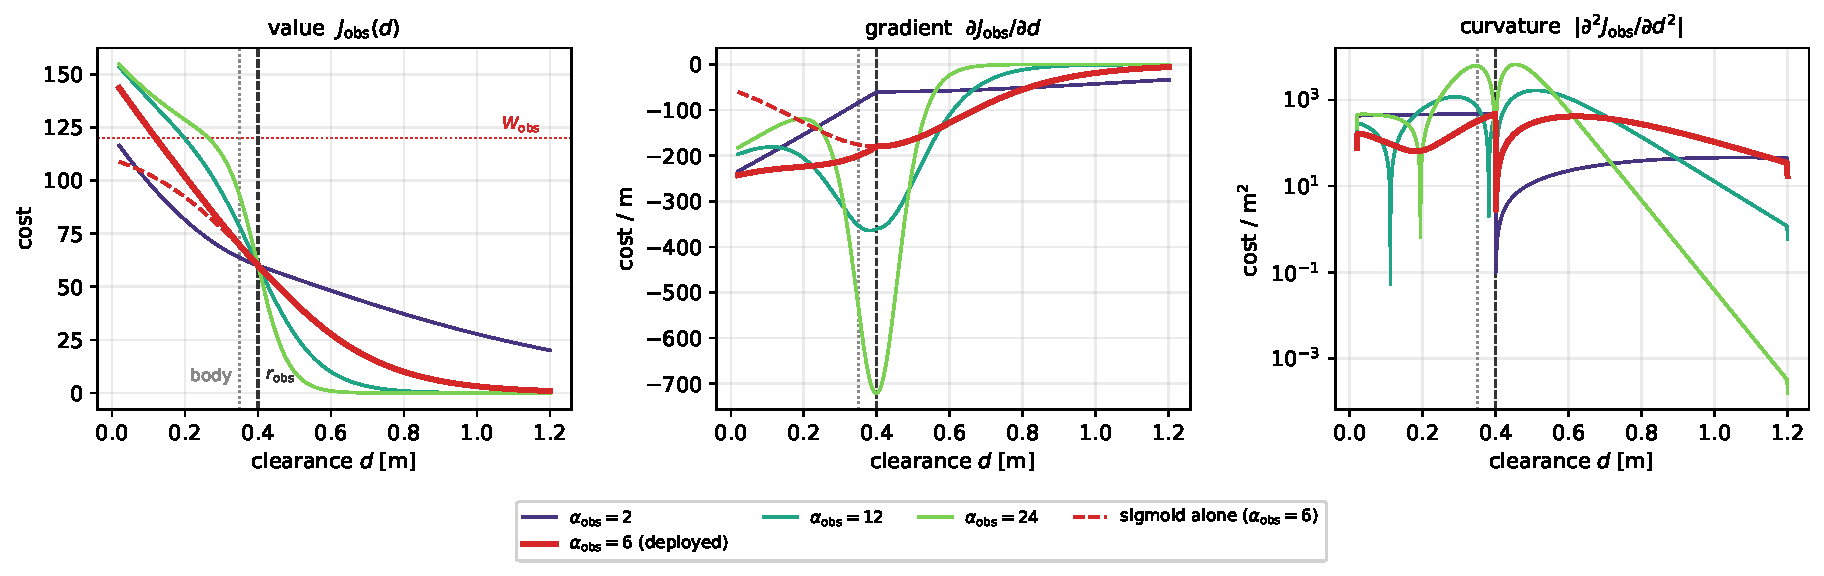
\includegraphics[width=\textwidth]{fig_barrier_shape.pdf}
  \caption{The hybrid penalty~\eqref{eq:barrier} against clearance, for four steepness values with the
  deployed $\aobs=\resAobsDep$ in bold ($\Wobs=\resWobsDep$, $\robs=\resObsRDep$~m; the dotted line marks
  the body radius). Dashed: the sigmoid zone alone at the deployed steepness, which saturates at $\Wobs$
  and whose gradient fades inside the obstacle --- the two defects the quadratic term repairs. Right, on a
  logarithmic scale: the curvature, which grows as $\aobs^2$ and is what degrades the conditioning of the
  NLP; the notches are sign changes. Evaluated through the same function the tracker builds into the NLP,
  not redrawn from the formula.}
  \label{fig:barriershape}
\end{figure}

Relaxing a hard constraint into a penalty has three consequences worth stating explicitly.
\emph{(i)}~The NLP is always feasible: no state constraint can render the problem unsolvable when the robot
is already too close to an obstacle, which for a real-time loop with no fallback trajectory is a genuine
robustness property. \emph{(ii)}~Safety is no longer guaranteed --- \eqref{eq:barrier} is not an exact
penalty, so a finite $\Wobs$ admits a finite violation, and Section~\ref{sec:l1} makes that statement
quantitative. A control-barrier formulation \cite{ames2019cbf} would recover the guarantee, at the price of
feasibility and of a harder NLP. \emph{(iii)}~The penalty is evaluated only at the $N+1$ discrete nodes, so nothing forbids the
continuous inter-sample trajectory from clipping a thin obstacle.

Point~\emph{(iii)} is worth checking rather than leaving as a caveat, because it is a one-line
computation. Between two consecutive nodes the robot advances at most $v_{x,\max}\Delta t$, against a
keep-out radius $\robs$, so the penalty is meaningful only while
\begin{equation}
  \frac{v_{x,\max}\,\Delta t}{\robs} \;<\; 1 .
  \label{eq:intersample}
\end{equation}
On the deployed profile the numerator is $\resVxMax\times\resDt$, i.e.\ about $14$~cm against
$\resObsRDep$~m of radius, so the ratio is $0.35$: safe, but a third larger than before the input
envelope was widened. It is reported rather than assumed because it is not invariant: it couples two
parameters tuned for unrelated reasons --- the sampling time of Section~\ref{sec:horizon} and the input
envelope of Table~\ref{tab:platforms} --- and lengthening $\Delta t$ to buy horizon walks it towards one.
Above one the obstacle term is absent between nodes, and geometric avoidance falls entirely to the
\astar{} layer on the inflated grid.

\paragraph{Sentinel padding.} $M$ is fixed. When fewer than $M$ returns lie inside the search radius, the
missing rows of the obstacle parameter are filled with a sentinel at $10^3$~m, whose contribution
to~\eqref{eq:barrier} is numerically zero. This apparently cosmetic detail is what allows the NLP to be built
\emph{once}: the number of terms, and therefore the sparsity pattern of the Jacobian and Hessian, never
changes between cycles, so the symbolic factorisation and the warm start remain valid regardless of how
cluttered the scene is.

\subsubsection{The obstacle as a true constraint: exact \texorpdfstring{$\ell^1$}{l1} penalty}
\label{sec:l1}

The alternative to a penalty in the cost is a constraint with a slack. The deployed code implements both,
selectable by a parameter: the obstacle becomes
\begin{equation}
  d(x_k,p_j)\;\ge\;\dsafe-s_{jk},\qquad s_{jk}\ge0,\qquad k=1,\dots,N,
  \label{eq:slack}
\end{equation}
with the slack penalised in the cost either linearly ($\rho_s\sum s$) or quadratically ($\rho_s\sum s^2$). The
question this settles is the one Section~\ref{sec:barrier} could only raise: at what weight, if any, does the
relaxation stop being a relaxation, so when the soft constraint becomes a hard one.

Penalising the slack in $\ell^1$ makes the penalty \emph{exact}: above a finite threshold --- $\mu^\star$,
the norm of the multipliers of~\eqref{eq:slack} at the solution --- the penalised and the constrained
problem share their minimisers and the slack vanishes identically, so beyond that weight the relaxation is no longer one.
On the deployed problem the slack is already identically zero at $\rho_s=\resRhoLoneZero$. Penalising in
$\ell^2$ never gets there at all: the slack decays as $1/\rho_s$ and the constraint is violated, however
slightly, at every weight.

That answer is also the reason the obstacle is left in the cost. A constraint that is genuinely hard can be
genuinely infeasible, and it becomes so exactly when the robot is already inside $\dsafe$ --- the one
situation in which a loop with no fallback trajectory must still return a command. This is
consequence~\emph{(i)} of Section~\ref{sec:barrier} read in the other direction: what the penalty gives up
in guarantees it buys back in always having an answer. Below the threshold nothing is gained either, since
the constraint is soft again and a soft constraint carrying one slack per node and per obstacle is
\eqref{eq:barrier} with more variables.

\paragraph{What it would cost to deploy.} Switching the obstacle from the cost to the constraints takes the
inequalities from $\resSolverIneqLow$ to $\resSolverIneqHigh$ and the iteration count up by a factor of
several. The deployed iteration cap would not suffice. This is also what makes the solver comparison of
Section~\ref{sec:solvercmp} possible at all: the same system can be placed in two regimes that differ by a
factor five in the number of inequalities, which is exactly the axis along which the standard advice on
solver choice is stated.

\subsubsection{Constraints}
\label{sec:constraints}

The deployed program carries only equality constraints and input bounds:
\begin{subequations}
\label{eq:cons}
\begin{align}
  & x_{k+1}-f(x_k,u_k)=0, && k=0,\dots,N-1, \label{eq:cons-dyn}\\
  & x_0-\hat x=0, \label{eq:cons-init}\\
  & v_{x,\min}\;\le\;u_{1,k}\;\le\;v_{x,\max}, && k=0,\dots,N-1, \label{eq:cons-vx}\\
  & |u_{2,k}|\le v_{y,\max},\qquad |u_{3,k}|\le\omega_{\max}, && k=0,\dots,N-1, \label{eq:cons-vyw}
\end{align}
\end{subequations}
with $v_{x,\min}=\resVxMin$~m/s, $v_{x,\max}=\resVxMax$~m/s, $v_{y,\max}=\resVyMax$~m/s and
$\omega_{\max}=\resOmegaMax$~rad/s (Table~\ref{tab:platforms}). Three remarks:

\begin{itemize}
  \item \textbf{No state constraints.} Neither the obstacle clearance nor the velocity states are
        constrained; the former is penalised, the latter are bounded implicitly because
        \eqref{eq:veldisc} is a convex combination of a bounded command and the previous velocity, so
        $v_{x,k}$ stays inside the input box for all $k$ whenever $v_{x,0}$ is --- which the state
        estimate does not guarantee, although on the deployed profile the degenerate lag of
        Section~\ref{sec:discretization} collapses~\eqref{eq:veldisc} to $v_{k+1}=u_k$ and the question
        does not survive the first node. The feasible set of the NLP is therefore a box intersected with
        an affine-in-$X$ manifold, and a feasible point is always trivially available (integrate any
        admissible input sequence).
  \item \textbf{The input box is asymmetric.} Constraint~\eqref{eq:cons-vx} admits reversing, but at half
        the forward speed, and~\eqref{eq:cons-vyw} caps strafing at the same fraction. Neither asymmetry
        is a safety derating applied to a symmetric machine: the lateral one is kinematic, since a biped
        strafes genuinely more slowly than it walks forward, while the backward one keeps the optimizer
        from adopting a retreat as a cheap shortcut at every stop. It is not free, however --- pricing
        the retreat above the wide forward arc is one of the three structural facts behind the livelock
        of Section~\ref{sec:localmin} --- and on hardware the bound may be tightened further to
        $v_{x,\min}=0$, since the LiDAR sees poorly behind the robot.
  \item \textbf{Bounds are parameters, not constants.} The three velocity limits enter the NLP as CasADi
        parameters, so the supervisor can shrink them at runtime (Section~\ref{sec:impl}) without
        rebuilding the problem --- to slow the robot down in a crowded area, for instance, or to open the
        envelope again in free space.
\end{itemize}

\subsubsection{Terminal ingredients and recursive feasibility}
\label{sec:terminal}

The deployed formulation carries no terminal set and no terminal constraint, so none of the standard
guarantees of nominal stability and recursive feasibility \cite{mayne2000constrained,chen1998quasi} applies.
Recursive feasibility is nevertheless \emph{structurally} present, for the reason given in
Section~\ref{sec:constraints}: with no state constraints, every input sequence in the box is admissible, so
the NLP always has a solution and the closed loop can never be aborted by infeasibility. What is lost is the
guarantee that the closed loop converges: the tracking term can decrease along a trajectory that walks into
a well of the obstacle penalty, and nothing but that penalty stops it.

It is worth saying plainly what that gap is. The controller plans $\resHorizonSeconds$~s ahead, executes the
first step of the plan, and then starts again from scratch. Nothing ties one plan to the next, so a sequence
of individually optimal plans need not go anywhere: each is the best available move inside a window that
never looked past its own edge. The standard device for closing the gap is a condition on the last predicted
state --- end every plan in a configuration that can be held indefinitely --- because the previous plan,
shifted forward by one step, is then always still executable. For a walking robot that configuration is
standing still, balance being the business of the policy of Section~\ref{sec:g1rl}, so the condition reads
$v(N)=0$: there must exist a braking trajectory inside the horizon.

On the plant used in this report that condition holds without being imposed. Section~\ref{sec:model} sets
$\tau_v=\tau_w=\resTauV$~s against $\Delta t=\resDt$~s, so the discrete lag coefficient is $\resLagDiscrete$
and the velocity update collapses to $v_{k+1}=u_k$: the model reaches zero velocity in a single sampling
step, from any speed. A braking trajectory therefore always exists and the guarantee comes for free --- for
a reason that belongs to the simulation and not to the robot.

Supplying it explicitly would cost very little. The constraint is imposed softly, as
\begin{equation}
  v_i(N)\;\le\;s_i,\qquad -v_i(N)\;\le\;s_i,\qquad s_i\;\ge\;0,\qquad i\in\{x,y,\omega\},
  \label{eq:terminal}
\end{equation}
with $\rho_s\sum_i s_i$ added to the cost: three slack variables and nine inequalities, against the
$\resNvar$ variables and $\resNcon$ constraints the program already carries, and all of them added once
rather than once per node. Penalising in $\ell^1$ is what makes the soft form acceptable; by the result
of Section~\ref{sec:l1} the constraint is effectively hard wherever it is satisfiable and yields instead of
aborting the loop where it is not. The deployed code implements it, selectable by a parameter; the deployed
profile leaves it off.

Measured with that parameter forced on, across cycles replayed from a recorded mission, the terminal slack
never leaves zero (maximum $\resTermSlackMax$, always admissible: \resTermFeasible), which is what the
degeneracy above predicts, and the optimal objective rises by between $\resTermAbsMin$ and $\resTermAbsMax$.
Those same cycles carry objectives ranging from $\resTermJMin$ to $\resTermJMax$, so the identical increase
reads as anything between $\resTermCostMin\%$ and $\resTermCostMax\%$ depending on which cycle is quoted:
the relative figure describes its own denominator rather than the constraint. The absolute cost is small,
roughly constant, and easy to account for; the plan has to predict its own braking, and the braking is
discarded at the next cycle anyway.

Where the constraint would earn its place is on an actuator that is not instantaneous. Repeating a cycle
with $\tau$ raised to $2$~s, so that the lag coefficient falls to $0.16$, produces the only strictly positive
terminal slack in this study: the horizon is no longer long enough to stop. On hardware, where $\tau$ is fixed by the locomotion policy and the gait
rather than chosen, $v(N)=0$ inside a fixed horizon is precisely the condition that ties the cruise speed to
the horizon length. This is the job currently done reactively, and outside the optimizer, by the adaptive
velocity ceiling of Section~\ref{sec:impl}.

\subsubsection{Reference trajectory: time-parametrised against path-parametrised}
\label{sec:pathfollow}

[DECIDERE SE MANTENERE QUESTO CAPITOLETTO, SE ACCORCIARLO O TOGLIERLO].
The deployed reference is a \emph{schedule}, not just a route: node $k$ of the horizon is the instant
$k\Delta t$ ahead, and the reference places it at the arclength the robot would have covered by then along
the smoothed \astar{} path at a fixed cruise speed,
\begin{equation}
  s_k=\min\!\left(s_0+v_{\mathrm{ref}}\,k\,\Delta t,\; L_{\mathrm{path}}\right),
  \label{eq:ref}
\end{equation}
interpolating inside the containing segment and taking the heading as the segment tangent. The $k\Delta t$
is the schedule, and it is what the robot is held to: if it cannot keep up, the reference runs away and the
tracking cost grows for reasons that have nothing to do with the quality of the control.

The clip against $L_{\mathrm{path}}$ is not a guard against indexing past the end of an array. When the
remaining path is shorter than $v_{\mathrm{ref}}N\Delta t$ the reference saturates at its last point, every
remaining node asks for the same position, and the tracking term becomes a terminal-position term: that is
the mechanism by which the controller decelerates into the local goal, and the formulation has no other. It
is inactive in transit --- the horizon covers about a metre and a half of a local path reaching some $6$~m
ahead --- and engages only on approach, which is also the only moment at which the terminal equilibrium
constraint of Section~\ref{sec:terminal} would have anything to ask for.

Setting $v_{\mathrm{ref}}$ below $v_{x,\max}$ is deliberate --- at $v_{\mathrm{ref}}=v_{x,\max}$ the tracker
saturates permanently and never settles onto the path --- and the price is structural: $\resVrefUnused\%$ of
the available forward speed is unreachable \emph{by construction}, and no cost weight recovers it, because
the reference never asks for it.

The alternative the theory offers is to drop the schedule and keep only the geometry: make the path abscissa
a decision variable and let the tracker choose how far to advance. What $\theta$ runs along is the
\emph{local} path --- the \astar{} route inside the window, ending at the boundary target of
Section~\ref{sec:astar} some $6$~m ahead --- refitted at every solve, with $\theta(0)=0$ at the robot and
$\theta=1$ at its far end. The deployed code implements this, with $\Delta\theta\ge0$, $\theta(N)\le1$ and a
progress term $\alpha_3(1-\theta)^2$ in the cost; $\bar z(\theta)$ is a polynomial rather than the
waypoint polyline, since $\theta$ is now differentiated through and a polyline has a discontinuous second
derivative at every node.

That the path is local is what makes the reformulation well posed, rather than a limitation of it. The robot
consumes about a third of it per horizon, so $\theta(N)\le1$ stays slack in transit and $(1-\theta)^2$ acts
as a pure incentive to get further along. Run instead along a path reaching all the way to a distant goal,
$\theta$ would advance by a few hundredths per horizon and offer nearly the same gradient at every node.

\begin{table}[htbp]
  \centering
  \small
  \caption{%
  Time-parametrised against path-parametrised reference, averaged over $\resPFcycles$ cycles replayed from
  the recorded run \resBag.}
  \label{res:tab:pf}
  \restab{pf}
\end{table}

Over $\resPFcycles$ moving cycles replayed from the recorded run the mean commanded speed rises from
$\resVxTime$ to $\resVxTheta$~m/s and the advance within one horizon from $\resAdvanceTime$ to
$\resAdvanceTheta$~m --- $\resAdvanceGain\%$ further at the same horizon, with $v_{x,\max}$ saturated on
nearly every step. The cruise speed does not reappear in another guise: $\theta$ is a variable, not a
hyperparameter.

It is paid for in iterations, and generously: $\resIterTime\to\resIterTheta$, close to a tripling. Part
of that is intrinsic --- $N+1$ more variables, as many more inequalities, worse conditioning. Part is not:
the warm start below guesses the inputs and the states and not the abscissa, so those $N+1$ variables enter
every solve cold, and the figure is an upper bound on the cost of the formulation rather than a measurement
of it. Reported as a trade rather than as an improvement, this remains the cleanest reformulation available
to the stack.

\paragraph{A trap worth documenting.} On cycles where the robot is stationary the comparison is
meaningless: $\theta$ advances without the dynamics being able to follow, and with a strong progress weight
one observes $\theta\to1$ while the robot stands still. The comparison is therefore restricted to cycles
with genuine motion --- not a numerical artefact but a modelling statement, since a path-parametrised
reference is only a reference if the dynamics can realise the progress it encodes.

\paragraph{Warm start.} The previous solution is reused as the initial guess for the inputs and the
states, by the standard shift-and-append rule
\begin{equation}
  U^{(0)}_{\text{new}} = \big[u^\star_1,\dots,u^\star_{N-1},u^\star_{N-1}\big],\qquad
  X^{(0)}_{\text{new}} = \big[x^\star_1,\dots,x^\star_{N},x^\star_{N}\big],
  \label{eq:warm}
\end{equation}
which is consistent to first order because the reference itself shifts by one step. Two safeguards protect
it: the guess is discarded after three consecutive solver failures, and whenever the optimal cost exceeds
five times the mean of the last seven solves. The second is about geometry rather than numerics --- a cost
spike means a new wall has entered the window and the \astar{} path now passes on the other side of it, so
the shifted guess lies in the basin of the \emph{old} minimum (Section~\ref{sec:bif}). Its computational
benefit is not measured here.

\subsubsection{Robust constraints: tightening from the measured prediction error}
\label{sec:robust}

[DECIDERE SE MANTENERE QUESTO CAPITOLETTO, SE ACCORCIARLO O TOGLIERLO].
Every constraint in~\eqref{eq:ocp} is imposed on the \emph{predicted} trajectory, and
Section~\ref{sec:prederr} measures how far the prediction drifts from what the robot actually does. A
clearance guaranteed in the plan is therefore not a clearance guaranteed on the floor. The standard remedy is
constraint tightening: replace $\dsafe$ with a margin $\gamma(k)$ that grows along the horizon,
\begin{equation}
  \big\|p_k-o_j\big\| \;\ge\; \dsafe+\gamma(k)-s_{jk}.
  \label{eq:tighten}
\end{equation}

The particularity of this project is that $\gamma(k)$ need not be postulated. It is read off the
$\resBetaQuantile$th percentile of the prediction error recorded in the bags, so the tube is derived from
data rather than from an assumption about the disturbance.

\begin{table}[htbp]
  \centering
  \small
  \caption{%
  Constraint back-off derived from the $95$th percentile of the measured prediction error. The offset at
  $k=0$ is subtracted: it is time misalignment, not model uncertainty, and including it would inflate the
  tube by a constant.}
  \label{res:tab:beta}
  \restab{beta}
\end{table}

Three properties hold by construction and were checked rather than assumed. $\gamma(0)=\resBetaZero$ exactly,
because at the first node the state is fixed by an equality and there is nothing to hedge against --- the
constraint is not tightened where tightening could only remove admissible motion. The margin is monotone
(\resBetaMonotone), as uncertainty is. And it reaches $\resBetaEnd$~m at the end of the horizon, the same
order as the safety radius itself. The offset at $k=0$ is subtracted before fitting, since
Section~\ref{sec:prederr} shows it to be time misalignment rather than model error, and including it would
inflate the whole tube by a constant.

\begin{table}[htbp]
  \centering
  \small
  \caption{%
  Effect of the tightening on the predicted trajectory.}
  \label{res:tab:robust}
  \restab{robust}
\end{table}

Measured on the predicted trajectory, the outcomes separate cleanly. Where $\dsafe+\gamma$ stays below the
clearance the trajectory already keeps, the constraint is inactive and correctly does nothing. Where it
bites, the predicted clearance increases by up to $\resRobustBestDelta$~m with the slack still exactly zero:
the margin is \emph{respected}, not violated and paid for --- which is the whole point of pairing the tube
with the $\ell^1$ relaxation of Section~\ref{sec:l1}, since a tube that asks more than $\mathcal{U}$ can
deliver makes the penalty yield instead of making the program infeasible.

\paragraph{The limit of this measurement, and what it says about the architecture.} The effect is
\emph{not} observable in the closed loop of this harness: the executed clearance comes out identical with and
without tightening. The reason is the architecture described in Section~\ref{sec:overview} --- the loop is
closed by tracking a look-ahead setpoint on the predicted trajectory with a proportional law, which washes
out fine differences between MPC solutions. The tightening guarantees the margin \emph{in the plan}, and that
is where it has been verified. This is not a limitation of the technique but of the test bench, and it is the
strongest argument in the report for applying $u^\star_0$ directly, as the receding-horizon principle
prescribes.

On the recorded industrial run the tightening is inert for a different and more instructive reason: at the
tightest cycles the robot sits about $0.6$~m from the obstacles and cannot move away. Raising $\dsafe$ grows
the slack but does not move the trajectory. The binding constraint is not the threshold, it is
$\mathcal{U}$ --- the same asymmetry found in Section~\ref{sec:l1} and quantified in Section~\ref{sec:kkt}.
Three independent measurements arrive at the same conclusion, which is the strongest form the report has for
saying that the input set, not the cost, is where this system is limited.


\subsubsection{On the absence of integral action}
\label{sec:integral}

The formulation has no integral action and no disturbance estimator: the state~\eqref{eq:state} is not
augmented with an input-disturbance model, and the reference is tracked in a purely
proportional--predictive sense. For a nominal plant this is immaterial, but any constant unmodelled input ---
a mis-identified $\tau$, a lateral drift of the gait, a slope --- produces a persistent offset from the path
rather than being integrated away. The offset is therefore a property of the formulation and not of the
tuning, and no choice of $Q$ removes it. Section~\ref{sec:mismatch} measures it;
Section~\ref{sec:discussion} discusses the standard remedy, state augmentation with an integrated tracking
error as in the velocity-form MPC of \cite{rawlings2017mpc}.

%=============================================================================
\section{Optimization procedure}
\label{sec:optproc}

\subsection{Problem dimensions and structure}
\label{sec:dims}

Table~\ref{res:tab:nlp} reports the size of the NLP against the horizon, measured on the deployed profile
rather than counted by hand.

\begin{table}[htbp]
  \centering
  \small
  \caption{%
  Size and sparsity of the NLP against the prediction horizon, from the deployed profile. Bold: the
  deployed configuration.}
  \label{res:tab:nlp}
  \restab{nlp}
\end{table}

At the deployed $N=\resN$ the program carries $\resNvar$ decision variables and $\resNcon$ constraints, of
which $\resNeq$ are equalities --- the dynamics plus the initial condition --- and $\resNineq$ are simple
bounds on the inputs. A further $\resNpar$ quantities enter as CasADi parameters: the measured state, the
reference, the sentinel-padded obstacle positions and the three velocity bounds. The problem is therefore
medium-scale, sparse, smooth and non-convex.

The constraint Jacobian is $\resJacDensity\%$ dense and the Hessian of the Lagrangian $\resHessDensity\%$.
Both densities fall as $N$ grows while the nonzero counts grow linearly, which is the signature of the
simultaneous parametrisation: the Jacobian of~\eqref{eq:cons-dyn} is block bi-diagonal, the Hessian block
tri-diagonal with the off-diagonal input blocks coming from the rate penalty, and nothing couples distant
stages. The linear-algebra cost of one interior-point iteration is consequently linear in $N$.

It is worth being explicit about what is \emph{not} in this table, because it shapes everything in
Section~\ref{sec:solvercmp}. There are no obstacle constraints: the $2M(N+1)$ obstacle terms all live in the
objective. There is therefore no obstacle multiplier, no non-trivial active set to identify, and the entire
inequality budget of the deployed program is $\resNineq$ box bounds on the inputs.

\subsection{Derivative computation}
\label{sec:deriv}

Every quantity the solver needs --- the gradient of the objective, the Jacobian of the constraints, the
Hessian of the Lagrangian --- is generated symbolically by CasADi and evaluated by generated code. The
alternative is finite differences, and the comparison is not a formality: it decides whether the second-order
method of Section~\ref{sec:solver} is affordable at all.

\begin{table}[htbp]
  \centering
  \small
  \caption{%
  Accuracy of the finite-difference gradient against the step size, measured against the AD gradient. The
  optimum sits at $h=1.49\times 10^{-8}$ one-sided (theory: $\sqrt{\varepsilon}=1.49\times 10^{-8}$) and
  $h=6.06\times 10^{-6}$ central (theory: $\varepsilon^{1/3}=6.06\times 10^{-6}$).}
  \label{res:tab:fd}
  \restab{fd}
\end{table}

At a representative solve the objective has $\resDerivNvar$ variables. One evaluation costs
$\resTimeF~\mu$s and one full gradient by reverse-mode algorithmic differentiation (AD) $\resTimeGrad~\mu$s,
i.e.\ $\resADratio$ objective evaluations --- a small constant, and crucially one that does not grow with the
number of variables. The same gradient by finite differences costs $\resFDforwardEvals$ evaluations one-sided
and $\resFDcentralEvals$ central, both growing linearly with $n$, and is less accurate at every step size:
the best relative error attainable is $\resFDforwardErr$ one-sided and $\resFDcentralErr$ central, against
machine precision for AD. The measured optimal steps coincide with the theoretical $\sqrt{\varepsilon_M}$ and
$\varepsilon_M^{1/3}$, $\varepsilon_M$ being the machine epsilon.

For a real-time loop the cost settles the question: central differences alone would consume
$\resFDcentralBudget\%$ of the $\resCycleBudget$~ms cycle budget, for a gradient that is worse, and the
fraction grows linearly with the horizon. The ratio itself is a micro-benchmark on
$\sim\!100~\mu$s timings and its second digit is not meaningful; what is stable, and is the point, is that it
remains a small constant.

\paragraph{The exact Hessian, and what it buys.} Because AD supplies exact second derivatives at a cost
comparable to the first, the full Newton system can be used rather than a quasi-Newton approximation.

\begin{table}[htbp]
  \centering
  \small
  \caption{%
  Interior-point iterations with the exact Hessian and with the limited-memory quasi-Newton approximation,
  on the same instance. Bold: the lower iteration count.}
  \label{res:tab:hess}
  \restab{hess}
\end{table}

On the same instance the exact Hessian converges in $\resIterExactHess$ iterations against $\resIterLBFGS$
for the limited-memory quasi-Newton approximation --- a $\resHessIterSaving\%$ reduction --- and both reach
the same objective value. The total time is closer than the iteration counts suggest, because each
quasi-Newton iteration is cheaper: this is the Newton / quasi-Newton trade-off in its textbook form,
measured without writing a solver. Section~\ref{sec:solvercmp} shows the other side of the same coin, where
the exact Hessian of a non-convex program produces an indefinite quadratic
program (QP) subproblem.

\subsection{Solver methodology}
\label{sec:solver}

The NLP is solved with IPOPT \cite{wachter2006ipopt}, a primal--dual interior-point method with a filter
line search. Writing the problem as $\min_z \phi(z)$ subject to $c(z)=0$ and $z^L\le z\le z^U$, the bounds
are replaced by a logarithmic barrier
\begin{equation}
  \varphi_{\mu_b}(z) \;=\; \phi(z) \;-\; \mu_b\sum_i\Big[\ln\!\big(z_i-z_i^L\big)+\ln\!\big(z_i^U-z_i\big)\Big],
  \label{eq:ipopt}
\end{equation}
the resulting equality-constrained problem is solved approximately by a Newton step on the perturbed Karush--Kuhn--Tucker (KKT)
system
\begin{equation}
  \begin{bmatrix}
    \nabla^2_{zz}\mathcal{L} + \Sigma & \nabla c(z)^{\!\top}\\
    \nabla c(z) & 0
  \end{bmatrix}
  \begin{bmatrix}\Delta z\\ \Delta\lambda\end{bmatrix}
  = -\begin{bmatrix}\nabla\varphi_{\mu_b}\\ c(z)\end{bmatrix},
  \label{eq:kkt}
\end{equation}
and $\mu_b$ is driven to zero. Each iteration requires one factorisation of the sparse symmetric indefinite
matrix in~\eqref{eq:kkt}, performed by MUMPS on the pattern of Section~\ref{sec:dims}.

There is a pleasing coincidence between~\eqref{eq:ipopt} and~\eqref{eq:barrier} that is worth naming: the
obstacle term of the deployed program is itself a barrier, and $\aobs$ plays the role of an inverse barrier
parameter. Steeper means better avoidance and worse conditioning, which is exactly the trade-off $\mu_b$
governs inside the solver. The difference is that IPOPT drives its own barrier parameter to zero along a
central path, whereas $\aobs$ is fixed by the tuning --- so the program is solved with a barrier that never
relaxes.

\subsection{Interior point against active set}
\label{sec:solvercmp}

The standard advice is that active-set methods win when the inequalities are few and interior-point methods
win when they are many. This stack can be moved between the two regimes without changing anything else,
because the obstacle formulation is switchable: with the obstacles in the cost the program carries
$\resSolverIneqLow$ inequalities, and with the obstacles as genuine constraints (Section~\ref{sec:l1}) it
carries $\resSolverIneqHigh$. That makes the advice testable rather than quotable.

\begin{table}[htbp]
  \centering
  \small
  \caption{%
  The same instance solved by a primal--dual interior-point method and by an SQP with an active-set QP
  solver, in both obstacle regimes. Both are started cold. Bold: the faster of the two.}
  \label{res:tab:solvercmp}
  \restab{solvercmp}
\end{table}

The rule does not reproduce: the active-set solver does not win even in the small regime, where the
interior-point method is already $\resSolverRatioLow\times$ faster. The \emph{direction} is confirmed --- the
margin widens to $\resSolverRatioHigh\times$ when the inequalities multiply --- so the break-even point, if
it exists, lies below the smallest regime into which this problem can be put.

Two cautions, without which the numbers would be misleading. First, the real advantage of an active set in
MPC is warm starting \emph{between consecutive solves}: the active set changes by a few rows per cycle and
the factorisation is reused, which is the online active-set strategy the method was designed for. Both
solvers are started cold here, deliberately, so as to favour neither --- which removes from the active-set
method precisely what makes it competitive in a receding-horizon loop. Second, the advice is stated for
convex programs, and this one is not.

\paragraph{A by-product that the theory predicts.} With the exact Hessian of the Lagrangian, the QP subproblem of the sequential quadratic
programming (SQP) method is repeatedly flagged indefinite. This is expected and instructive: a non-convex
program can produce a non-convex QP, and a non-convex QP has no unique solution. It is exactly the reason a
Gauss--Newton Hessian --- positive semi-definite by construction --- is the standard recommendation for SQP,
and it is the counterpart of the result in Section~\ref{sec:deriv}, where the same exact Hessian was the
better choice inside an interior-point method. The two are not in contradiction: an interior-point method
regularises the indefinite system in~\eqref{eq:kkt}, an SQP must solve the QP.

\paragraph{A methodological note.} On a first run the SQP appeared to converge in a single iteration to a
worse objective than IPOPT. Comparing the time of two solves that terminate at \emph{different} minima means
nothing, and the tool now verifies that the two objectives agree before declaring a winner. Table
\ref{res:tab:solvercmp} reports that check in its last column.

\subsection{Optimality conditions on the deployed problem}
\label{sec:kkt}

Everything above assumes that what the solver returns is a solution. That is a verifiable statement, and this
section verifies it on cycles extracted from a recorded mission rather than on a synthetic instance.

\begin{table}[htbp]
  \centering
  \small
  \caption{%
  Optimality diagnostics at sampled cycles of the recorded run \resBag. ``active'' counts equalities and
  active bounds together; ``rank'' is the rank of the Jacobian of the active constraints, so LICQ holds
  when the two coincide.}
  \label{res:tab:kkt}
  \restab{kkt}
\end{table}

At $\resKKTcycles$ sampled cycles, the linear independence constraint qualification (LICQ) holds at every one (\resLICQalways) --- the rank of the Jacobian of
the active constraints equals their number --- so the KKT multipliers exist and are \emph{unique}. Strict
complementarity holds at every one (\resStrictAlways), which means the critical cone coincides with the null
space of the active Jacobian and the second-order condition can be checked exactly rather than
conservatively. And the reduced Hessian is positive definite on that cone at every cycle
(\resSOCalways), the smallest projected eigenvalue over the profile being $\resLambdaMinWorst$. Taken
together these are a certificate of strict local optimality, which is the most that can be claimed for a
non-convex program.

\paragraph{The result worth reporting is the shape of the active set.} The critical cone contracts from
$\resConeFirst$ dimensions at the first sampled cycle to $\resConeLast$ at the last: with $\resNvar$
variables and $\resActiveLast$ active constraints, almost no freedom remains. The controller moves from
\emph{cost-driven} to \emph{constraint-driven} over the course of the mission, and towards the end it does
not so much choose the trajectory as undergo it. The breakdown of the active bounds explains it: the lateral
and yaw limits are saturated on essentially every step of the horizon, and the non-negativity of $v_x$ on
nearly all of them.

This is the quantitative form of the statement made three times elsewhere in this report. A lateral bound of
$v_{y,\max}=\resVyMax$~m/s does not \emph{limit} a degree of freedom, it \emph{removes} it. Section
\ref{sec:l1} found the residual infeasibility of the tightened obstacle constraint to be a property of
$\mathcal{U}$; Section~\ref{sec:robust} found the tube inert on the real run for the same reason; and here
the same fact appears as a critical cone of dimension $\resConeLast$. No choice of cost weights can return
what the input set has taken away.

\paragraph{Two traps in reading multipliers out of a modelling layer.} Both were met here and both would have
produced quietly wrong numbers. CasADi's \texttt{Opti} canonicalises every constraint as
$\mathrm{lbg}\le g(z)\le\mathrm{ubg}$ and \emph{absorbs into the bounds} any parametric right-hand side, so
$X_{:,0}=\hat x$ becomes $g=X_{:,0}$ with $\mathrm{lbg}=\mathrm{ubg}=\hat x$: evaluating $|g|$ on those rows
returns the state, not the residual, which is always $g-\mathrm{lbg}$. And two distinct rows can share the
same expression with different bounds --- $u_{1,k}\ge0$ and $u_{1,k}\le v_{x,\max}$ are both the row
$u_{1,k}$ --- so activity must be decided on the distance from the bound, not on $|g|\approx0$, or both sides
of every box are counted active.

\subsection{Implementation and configuration}
\label{sec:impl}

The program is built once, symbolically, and every quantity that changes between cycles is a parameter rather
than a constant: the measured state, the reference, the sentinel-padded obstacle positions and the three
velocity bounds. Consequently the expression graph, the derivative code and the sparsity patterns are
generated exactly once at start-up, and a cycle only writes numbers into parameter slots and calls the
solver. The graph is flattened so that the interpreter overhead of a problem with thousands of elementary
nonlinear operations does not dominate. The first solve after start-up therefore pays a one-off construction
cost, which is the single deadline violation of an entire run and is absorbed by holding the robot still
during initialisation.

The solver options are deliberately austere, with a low iteration cap: a non-converged iterate is still
usable as a reference by the downstream setpoint stage, which is a property of the architecture of
Section~\ref{sec:overview} and would not hold if $u^\star_0$ were applied directly. The real-time protection
lives in the supervisor rather than inside IPOPT --- a solver whose behaviour depends on a wall-clock limit
is not deterministic and cannot be characterised. The supervisor clears the warm-start cache on solver
failure, falls back to a zero command after repeated failures, and can shrink the velocity bounds through the
parameter interface when the failure rate rises.

%=============================================================================
\section{Performance analysis}
\label{sec:performance}

\subsection{Experimental setup}
\label{sec:setup}

All results in this section are produced by an offline harness that imports the \emph{production} modules ---
the grid, the \astar{} planner and the MPC tracker --- so every number is generated by the deployed
formulation and the deployed solver, not by a re-implementation. Two kinds of experiment are used and they
answer different questions.

\emph{Replay from recorded missions.} The bag \resBag{} contains a full run of the G1 in the industrial world:
the poses, the LiDAR scans, the \astar{} paths and the MPC predictions as they were published. Replaying it
gives real operating points, with the geometry and the clutter the robot actually met, and is what
Sections~\ref{sec:prederr} and~\ref{sec:kkt} use. It cannot answer counterfactual questions.

\emph{Closed-loop synthetic scenarios.} For counterfactuals --- what if the horizon were shorter, what if the
weights were different --- the harness runs full missions in scripted worlds, with a ray-marched planar
LiDAR and the discrete model of Section~\ref{sec:discretization} as the plant. This is what
Sections~\ref{sec:horizon}, \ref{sec:nc} and~\ref{sec:pareto} use. Two of these worlds recur: a narrow gap
and a U-shaped trap.

A third family is used only in Section~\ref{sec:nonconvex}, because it probes a different layer. The worlds
\texttt{long\_wall}, \texttt{horseshoe} and \texttt{dead\_end} each place a \emph{non-convex} obstacle
between the robot and the goal --- a wall long enough that its ends leave the window, a horseshoe, and a
corridor closed at the far end. They are run with \emph{limited perception}: the robot sees only out to the
LiDAR range and only what is not occluded, and accumulates what it sees. That last detail is not a refinement
but the whole experiment, because with the obstacle known in advance the discrete planner never enters the
trap and the failure under study does not occur.

A correction to an earlier reading of the second family, which the report would be weaker for omitting.
Previous versions of this section reported that in the U-trap the minimum clearance came out at zero in
essentially every configuration tested, and concluded that the world discriminated on time and computation
but said nothing about safety. That reading was an artefact of the harness, not a property of the world: the
replay loop selected its setpoint at a look-ahead distance that no longer matched the deployed one, so the
fallback proportional law took over and the output of the MPC was discarded on every cycle. With the
look-ahead read from the profile, the grazing configurations are confined to the very short horizons ---
$7$ of the $25$ combinations in the U-trap, all of them at $N\Delta t\le 2$~s, and none at all in the narrow
gap --- and the median clearance is $0.856$~m. The clearance axis therefore does discriminate, and
Section~\ref{sec:horizon} reads it. The general lesson is worth keeping: a harness that silently bypasses the
controller under test reports plausible numbers, and the only thing that exposed it was a quantity ---
clearance --- that had no business being identical across configurations.

\subsection{The cost landscape, and why this is not a potential field}
\label{sec:landscape}

Before the campaigns, it is worth looking at the object all of them are about. Fig.~\ref{fig:landscape}
draws, over the world plane of the recorded industrial run, the cost of \emph{being} at a point,
\begin{equation}
  c(p) \;=\; \underbrace{\text{tracking cost of the reference}}_{\text{the }Q\text{ block of Eq.~\eqref{eq:cost}}}
        \;+\; \underbrace{\Jobs(p)}_{\text{Eq.~\eqref{eq:barrier}}},
  \label{eq:landscape}
\end{equation}
with the executed trajectory, the \astar{} reference and one MPC horizon drawn on the surface, and the
per-cycle optimal cost $J^\star$ underneath.

\begin{figure}[htbp]
  \centering
  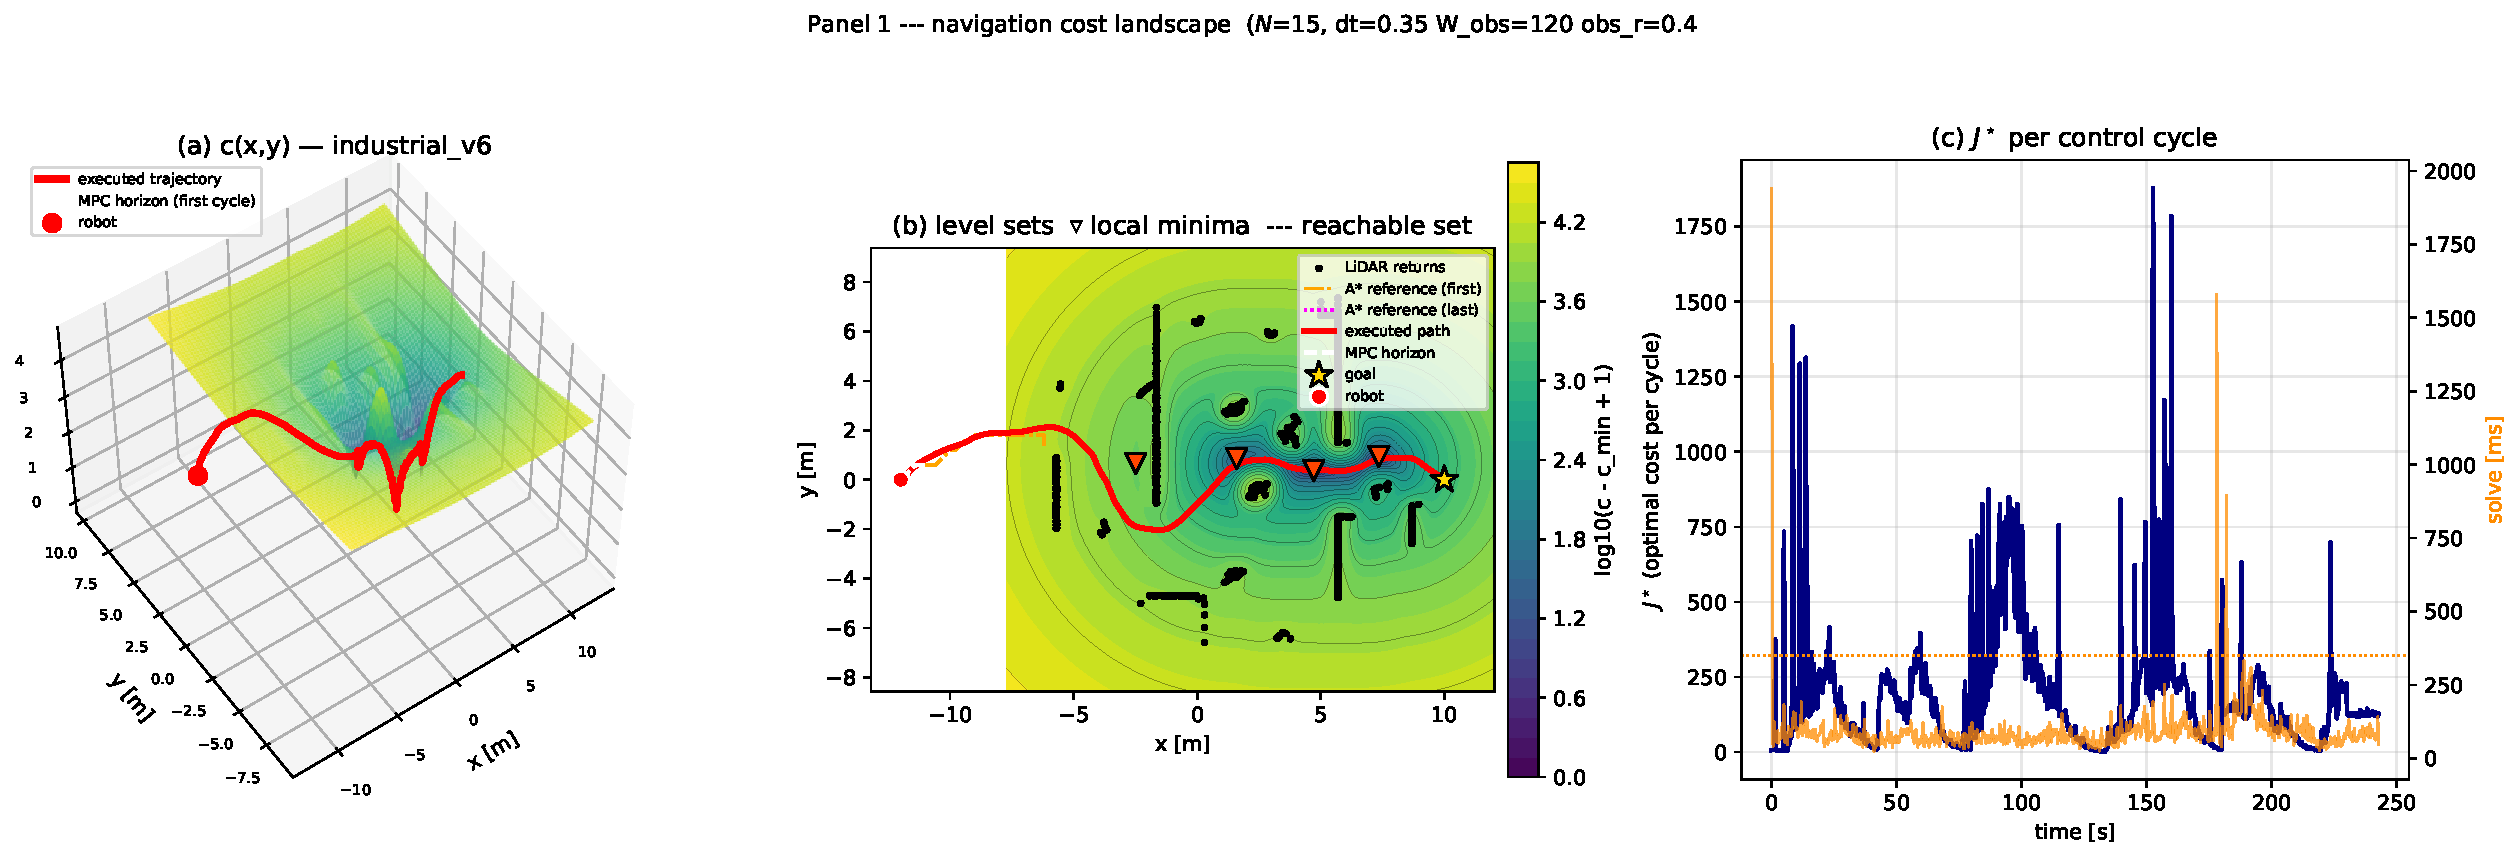
\includegraphics[width=\textwidth]{cost_landscape}
  \caption{The navigation cost landscape of the recorded run \resBag. \textbf{(a)} the surface
  $c(p)$ of Eq.~\eqref{eq:landscape} over the world plane, with the executed trajectory (red) and one MPC
  horizon (dashed) drawn \emph{on} the surface: the obstacle term raises a ridge along every wall of the
  plant, the tracking term forms the valley along the \astar{} reference. \textbf{(b)} the same field as
  level sets, with the local minima marked and the shaded region showing the set reachable within one
  horizon under $\mathcal{U}$ --- the constraint, not the cost, is what excludes most of the plane.
  \textbf{(c)} the optimal cost $J^\star$ of each control cycle, and the solve time beside it. The point
  worth noticing is in panel~(a): \emph{the trajectory does not follow steepest descent}, and climbs the
  surface wherever doing so lowers the sum over the horizon.}
  \label{fig:landscape}
\end{figure}

The distinction that figure makes visible is the one between $c$ and $J$, and it is the reason the stack
uses an optimizer rather than a reactive law. The quantity plotted is $c$, the cost of occupying a point;
what the program minimises is
\begin{equation}
  J(U) \;=\; \sum_{k=0}^{N} c(p_k) \;+\; \text{input terms},
  \label{eq:candJ}
\end{equation}
the cost of a whole \emph{trajectory}. A controller that descended $c$ pointwise would be an artificial
potential field, and it would stop at the first local minimum of the surface. The MPC minimises the sum
along a horizon instead, so it can --- and in panel~(a) visibly does --- move \emph{uphill} on $c$ when that
buys a lower total. This is what lets the same cost function carry the robot out of a concave pocket, and it
is the sense in which the obstacle term of Eq.~\eqref{eq:barrier} is a penalty inside an optimization
problem rather than a repulsive force.

One further reading, which anticipates Section~\ref{sec:kkt}. The shaded region in panel~(b) is not a level
set of the cost: it is the set of points the robot can reach within one horizon given $\mathcal{U}$. Most of
the plane is excluded from the decision by the \emph{constraints}, not by the objective --- and on this
platform, with $v_{y,\max}=\resVyMax$~m/s against a forward bound of $\resVxMax$~m/s and reversing
admitted only at a fraction of that, the region is markedly asymmetric about
the heading. The cost is what chooses inside it; the input set is what draws it.

\subsection{Prediction error: the model against the plant}
\label{sec:prederr}
% alias: Sezioni 2.3.3 e 3.3.8 rimandano qui come "model mismatch".
\label{sec:mismatch}

The most consequential measurement in this report requires no new experiment: the bags already contain, at
each cycle, the trajectory the MPC predicted, and the poses the robot subsequently reached. Comparing the
prediction published at time $t$ with the pose measured at $t+k\Delta t$, over $\resPredCycles$ usable
cycles, gives the growth of the prediction error along the horizon.

\begin{table}[htbp]
  \centering
  \small
  \caption{%
  Open-loop prediction error along the horizon, over $\resPredCycles$ cycles of the recorded run \resBag.}
  \label{res:tab:pred}
  \restab{pred}
\end{table}

\begin{figure}[htbp]
  \centering
  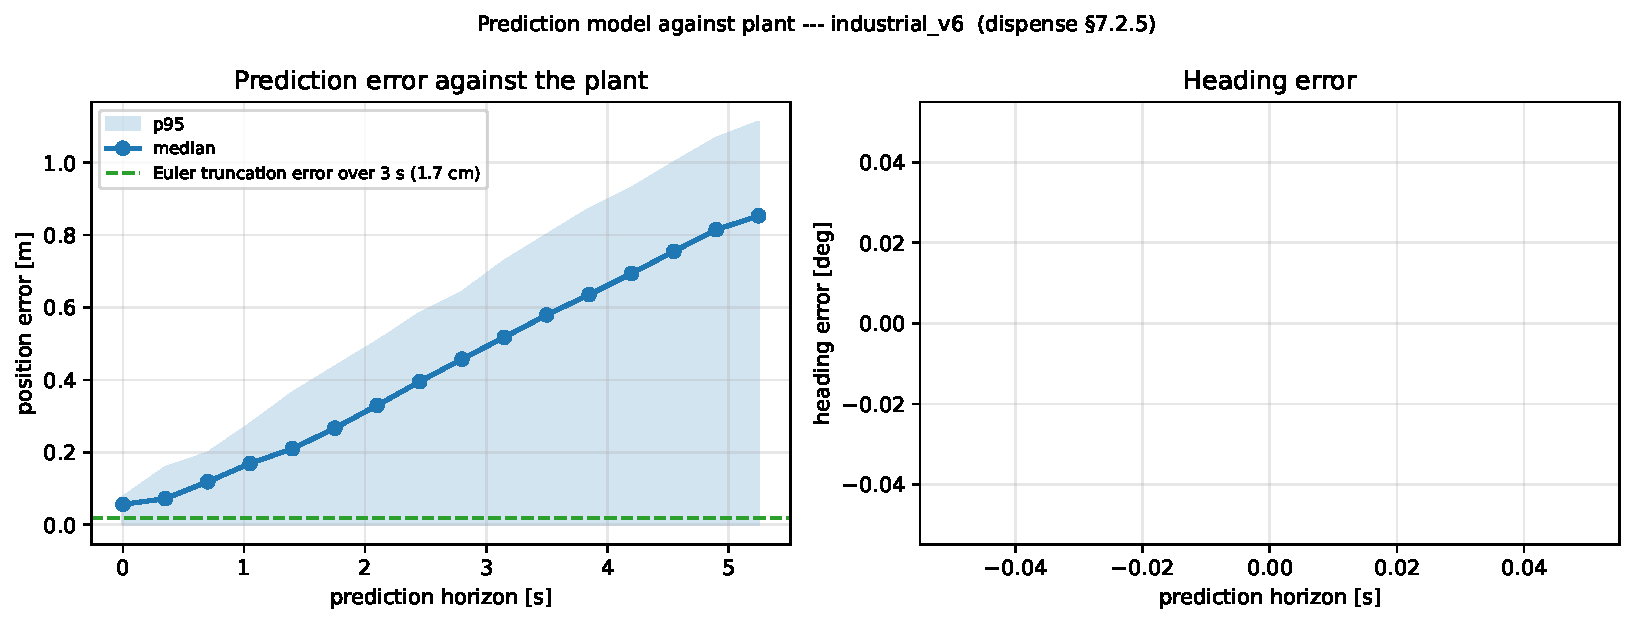
\includegraphics[width=0.92\textwidth]{prediction_error}
  \caption{Prediction error against the position along the horizon, over $\resPredCycles$ cycles of the
  recorded run \resBag: median and $95$th percentile. The residual at $k=0$ is time misalignment between the
  instant the prediction is published and the instant the pose is sampled, not model error, and is subtracted
  before quoting the divergence.}
  \label{fig:prederr}
\end{figure}

The residual at $k=0$ is $\resPredOffset$~m and is \emph{not} model error: at the first node the predicted
state \emph{is} $\hat x$, imposed as an equality constraint. It measures the delay between the instant the
prediction is published and the instant the pose is sampled, and it is subtracted to isolate the genuine
divergence, which is $\resPredDivergence$~m at the end of the horizon.

Put beside Section~\ref{sec:discretization}, that number closes a circle and is uncomfortable. The divergence
is $\resPredVsEuler$ times the truncation error of forward Euler over the same window, and
$\resPredVsMidpoint$ times that of the mid-point rule now deployed. The integrator was never the dominant
term. Upgrading it improved the arithmetic of the prediction by a factor $\resIntegratorGain$ and left the
closed loop essentially unchanged, and this is why: what limits the prediction is not how the model is
integrated but that the model is a planar holonomic agent and the plant is a twenty-nine-degree-of-freedom
humanoid walking. The correct response is not a better integrator but either a better model or, more
cheaply, an explicit account of the residual --- which is what the constraint tightening of
Section~\ref{sec:robust} does with this very curve.

\subsection{Regularity of the solution and the left--right bifurcation}
\label{sec:bif}

The program is non-convex, so its solution need not depend continuously on the data. The place where this is
visible is an obstacle centred on the reference: the problem then admits two symmetric local minima --- pass
left, pass right --- and the MPC law is a well-defined function of the state only as long as one of them
dominates.

The experiment solves the \emph{same} instance twice, from a left-biased and a right-biased initial guess,
and measures the distance between the two returned trajectories as the obstacle weight is swept.

\begin{table}[htbp]
  \centering
  \small
  \caption{%
  Left-biased against right-biased solve of the same instance, against the barrier weight. The separation
  is the distance between the two returned trajectories: a value at solver tolerance means the two guesses
  converged to the same minimum.}
  \label{res:tab:bif}
  \restab{bif}
\end{table}

\begin{figure}[htbp]
  \centering
  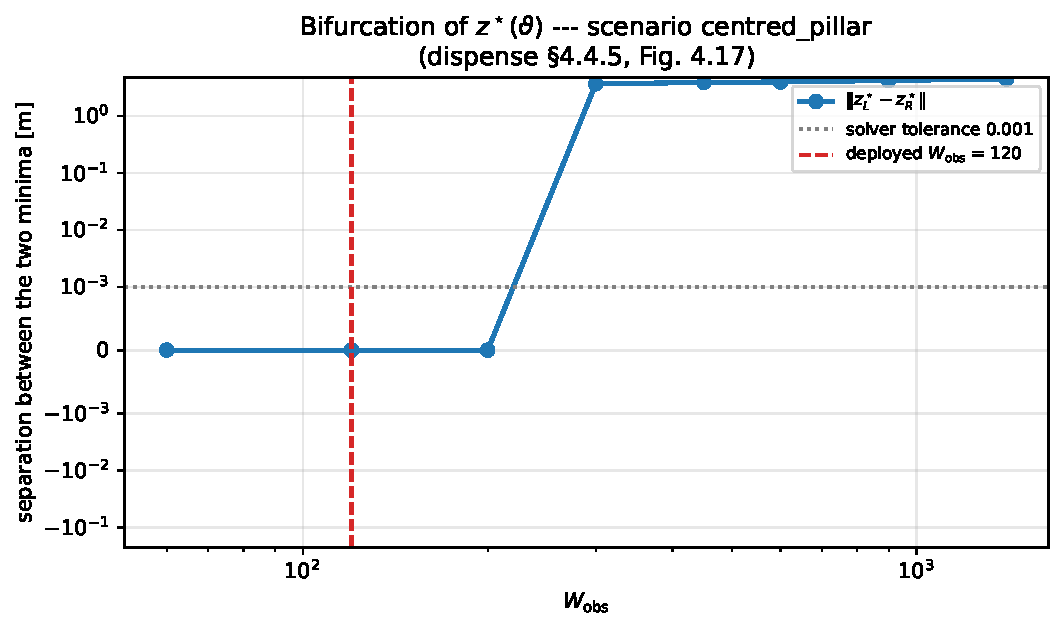
\includegraphics[width=0.92\textwidth]{bifurcation}
  \caption{Separation between the trajectories returned from a left-biased and a right-biased initial guess,
  against the obstacle weight $\Wobs$. Below the transition the two guesses collapse onto the same minimum
  and the control law is a regular function of the state; above it they do not.}
  \label{fig:bif}
\end{figure}

The transition sits between $\Wobs=\resBifLow$ and $\resBifHigh$, and the deployed weight
($\resWobsDep$) is below it: at the tuning in use the minimiser is unique and regular in $x_0$. Two further
readings follow. Past the transition the two minima are \emph{not} equivalent --- their objective values
differ by up to $\resBifCostGap\%$ --- so the initial guess decides not only which side the robot passes but
how much the manoeuvre costs. And on the hardest cycle of the recorded run, cycle $\resBifBagCycle$, the
sweep never bifurcates (\resBifBagEver) even far above the threshold, which Section~\ref{sec:kkt} explains:
that cycle has a critical cone of dimension one, and with a single remaining degree of freedom there is no
room for two distinct basins. Constraint saturation kills the bifurcation before the weight can create it.

A practical consequence for the deployed code: the guard that clears the warm-start cache when the objective
jumps between cycles is protecting against a phenomenon that does not occur at these weights.

\paragraph{Seeing it in the decision space.} The sweep above measures the bifurcation; Fig.~\ref{fig:decplane}
shows it. Plotting a function of $\resNvar$ variables requires choosing a two-dimensional section, and a
random one would almost surely contain nothing: the plane here is built to contain the structure. The program
is solved twice, warm-started to the left and to the right, giving the two minima $z^\star_L$ and $z^\star_R$;
the initial iterate supplies a third anchor; and the affine plane through those three points contains both
minima \emph{by construction}. The IPOPT iterates then project onto it exactly, since orthogonal projection
onto an affine subspace is exact --- which is why this figure can show the path from $z^0$ to $z^\star$ and
Fig.~\ref{fig:landscape} cannot.

\begin{figure}[htbp]
  \centering
  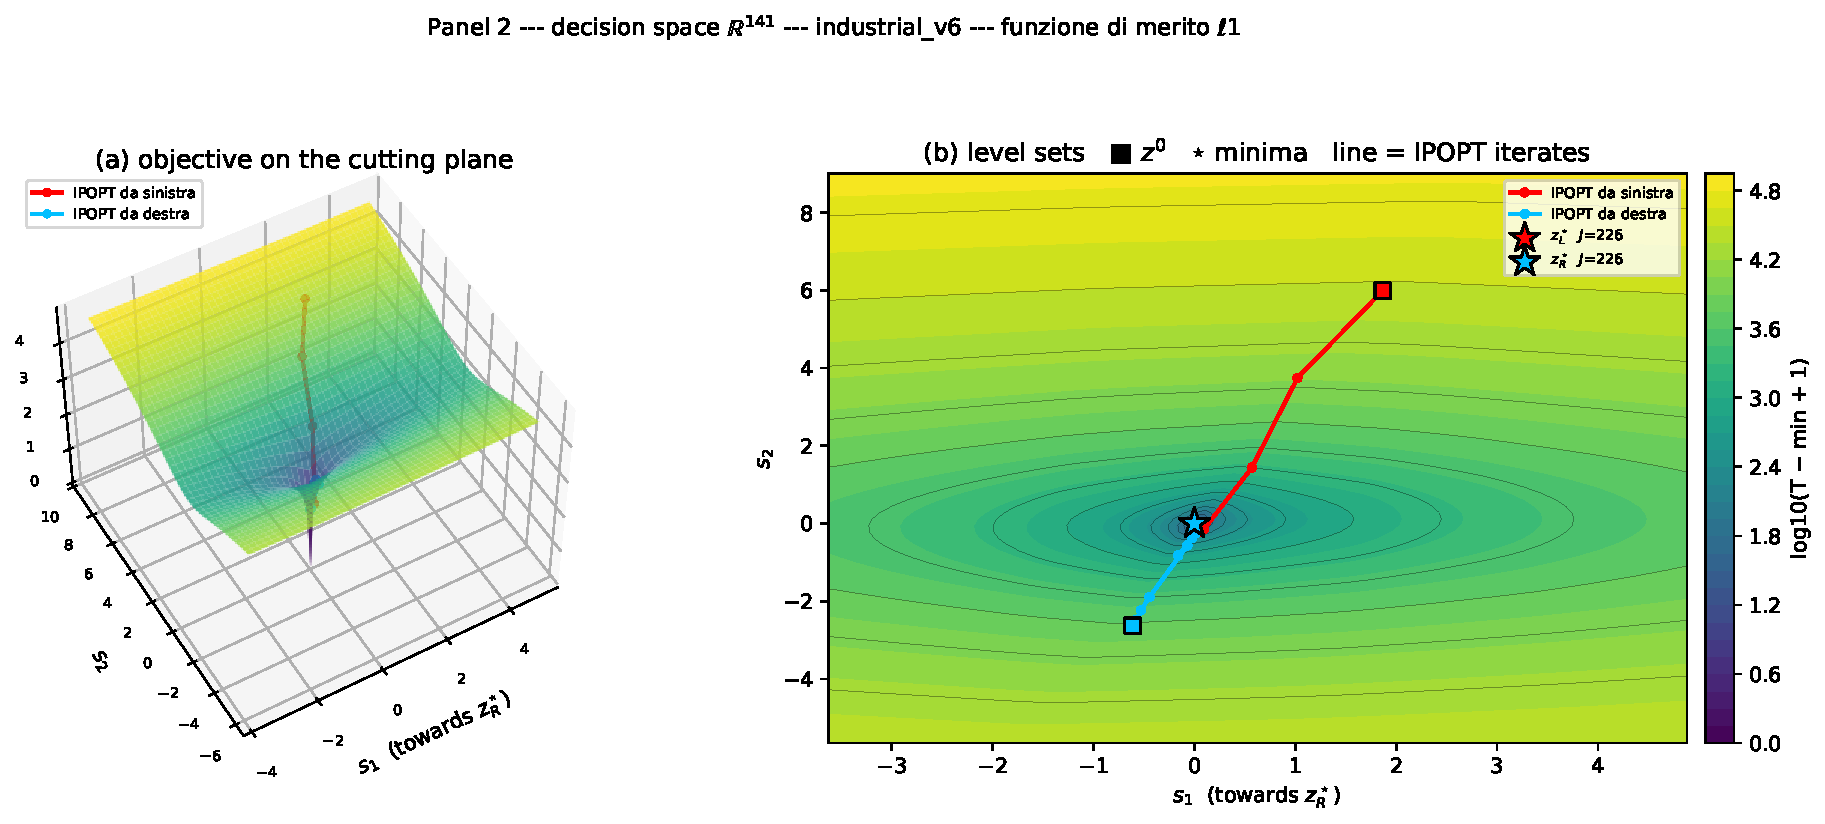
\includegraphics[width=\textwidth]{decision_plane}
  \caption{The objective in the decision space $\R^{\resNvar}$, on a plane constructed to contain both local
  minima of the recorded cycle. \textbf{(a)} the surface; \textbf{(b)} its level sets with the two minima
  ($\star$), the initial iterate ($\blacksquare$) and the IPOPT iterates joining them. What is plotted is not
  the objective $f$ but the $\ell^1$ merit function $T_1(z)=f(z)+\sigma\|c(z)\|_1$: in the simultaneous
  parametrisation $X$ and $U$ are independent variables tied by the dynamic equalities, so a generic point of
  the plane is \emph{not} dynamically feasible and a plot of $f$ alone would show a landscape the solver never
  traverses. The merit function is what the line search actually decreases.}
  \label{fig:decplane}
\end{figure}

The choice of what to plot is itself a point about the formulation. Under multiple shooting the states are
decision variables, so almost every point of the plane violates Eq.~\eqref{eq:cons-dyn}; the objective is
defined there but meaningless, because no trajectory of the plant corresponds to it. The $\ell^1$ merit
function --- objective plus weighted constraint violation --- is defined everywhere, agrees with the objective
on the feasible manifold, and is the function whose decrease the line search enforces. Plotting it is the
honest choice, and it also makes the figure legible: the funnel visible in panel~(b) is the constraint
violation being driven to zero, and the iterates run down it before moving along the bottom towards the
minimum. That two-phase shape is the geometry of a filter line-search method, and it is the same mechanism
that Section~\ref{sec:l1} exploits when it makes the obstacle constraint exact.

\subsection{Prediction horizon and sampling time}
\label{sec:horizon}

The two horizon parameters are not interchangeable. The product $N\Delta t$ sets how far the controller sees,
$N$ alone sets how much the solve costs, and $\Delta t$ alone sets how faithfully the prediction is
integrated. They were therefore swept jointly, in closed loop, over $\resHorizonConfigs$ configurations.

\begin{table}[htbp]
  \centering
  \small
  \caption{%
  Horizon campaign, scenario \texttt{narrow\_gap}. Bold: the deployed configuration $N=15$, $\Delta
  t=0.35$~s.}
  \label{res:tab:horizon:narrowgap}
  \restab{horizon_narrowgap}
\end{table}
\begin{table}[htbp]
  \centering
  \small
  \caption{%
  Horizon campaign, scenario \texttt{u\_trap}. Bold: the deployed configuration $N=15$, $\Delta t=0.35$~s.}
  \label{res:tab:horizon:utrap}
  \restab{horizon_utrap}
\end{table}

\begin{figure}[htbp]
  \centering
  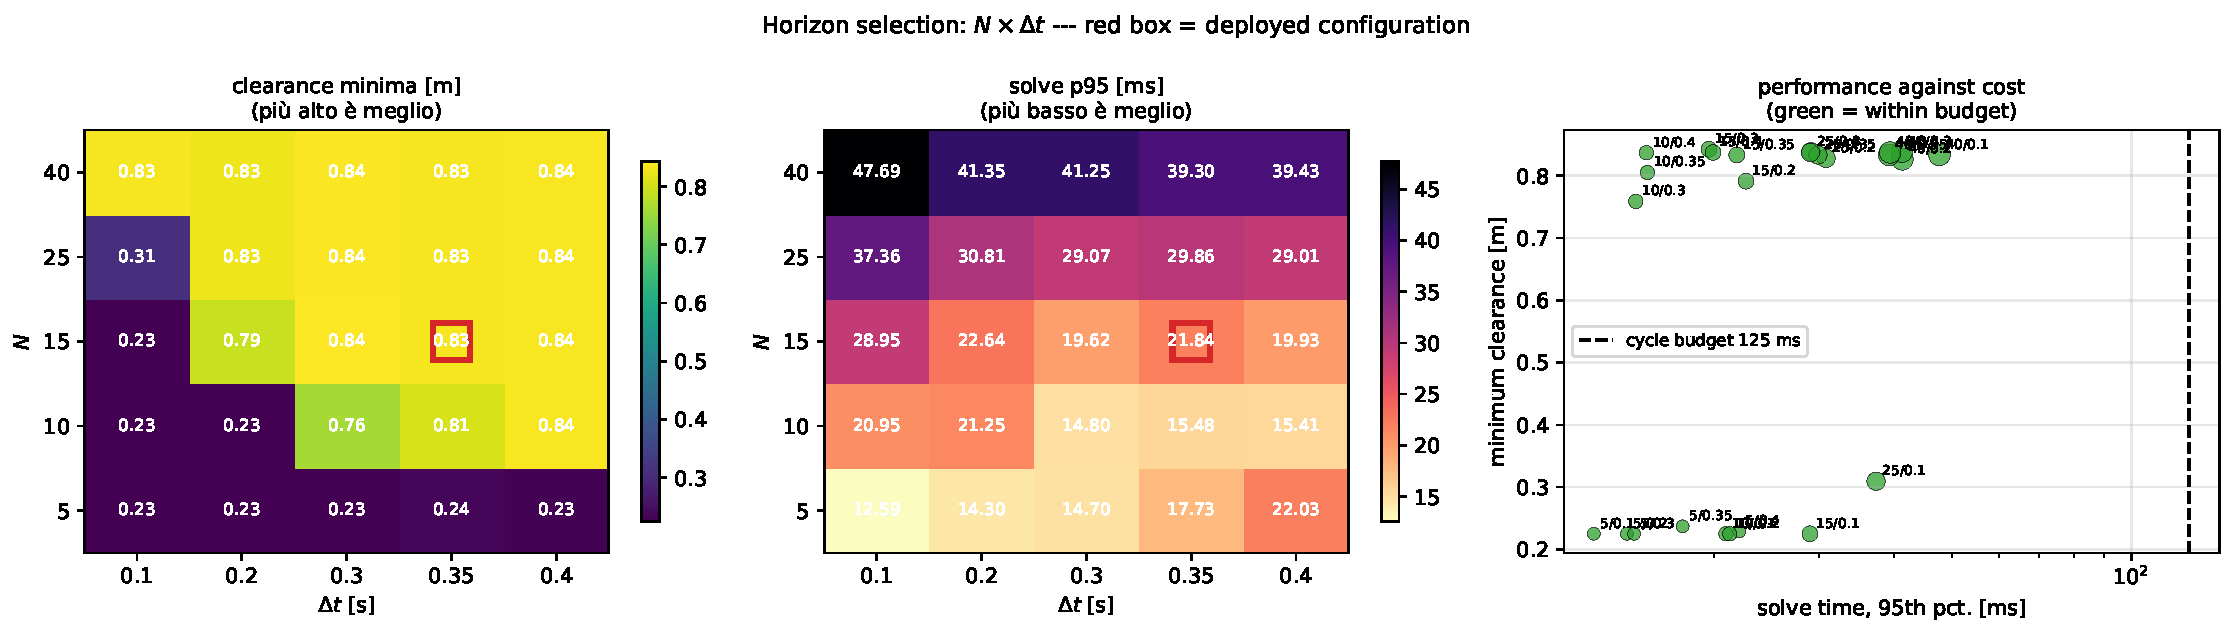
\includegraphics[width=\textwidth]{horizon_sweep}
  \caption{Joint sweep of the prediction horizon $N$ and the sampling time $\Delta t$ in closed loop. The
  deployed configuration is marked. Cost is governed by $N$; closed-loop quality is governed by the product
  $N\Delta t$, and not monotonically.}
  \label{fig:horizon}
\end{figure}

The result is a trade and not a dominance, and stating it as one matters because an earlier version of this
section did not. Grouped at $N\Delta t=\resHorizonSplit$~s, the short-horizon configurations reach the goal in
$\resHorizonLowT$~s against $\resHorizonHighT$~s for the long-horizon ones --- so on time the short horizon
wins, and by a wide margin. On safety the ordering reverses, and far more sharply: the worst-case clearance
in the short group is $\resHorizonLowC$~m against $\resHorizonHighC$~m in the long one. Every configuration
that grazes has $N\Delta t\le 2$~s. The short horizon is not cheaper at the same quality; it is faster
because it cuts corners, and at two seconds of look-ahead it cuts them until it touches.

The mechanism behind the time half is the one that produces the failure of Section~\ref{sec:localmin}: the
reference extends over a path that the discrete layer will replan anyway, so a longer horizon commits the
controller to tracking a target already due to change. What the clearance half adds is the limit of that
argument. Delegating avoidance to the discrete layer works only while the layer is fast enough and the world
is static; the horizon is what buys the margin when it is not. Section~\ref{sec:nc} separates the explanation
from its competitor --- simply too many decision variables --- and reports which one the data supports.

Ranking the configurations on the three objectives that matter (time to goal, worst-case clearance, tail
solve time) leaves $\resHorizonNondom$ non-dominated points, and the deployed $N=\resN$, $\Delta t=\resDt$~s
is \emph{dominated} (\resHorizonDepNondom) --- but by exactly one configuration, and narrowly:
$N=15$, $\Delta t=0.30$~s reaches the goal in $16.9$~s against $17.0$, with clearance $0.814$~m against
$0.811$, at $20.4$~ms of tail solve time against $\resHorizonDepTail$~ms. Three milliseconds and three
millimetres are not a reason to retune.

The cheapest non-dominated point is a different matter and must not be read as a recommendation. It is
$N=\resHorizonCheapN$, $\Delta t=\resHorizonCheapDt$~s at $\resHorizonCheapPtail$~ms, which survives the
ranking only because non-dominance is a weak relation: it is faster and cheaper, and it has zero clearance.
It is in the front because nothing beats it on all three axes at once, not because it is deployable.

Where the horizon genuinely can be improved is by adding the third parameter, and Section~\ref{sec:nc}
does. Sweeping $N$, $\Delta t$ and the control horizon $\Ninput$ jointly over three scenarios finds seven
configurations that dominate the deployed one, the best of them halving the tail solve time at identical time
to goal and identical clearance. That result comes from the control horizon, not from the prediction horizon,
which is the distinction this section cannot make on its own.

A caution on all of the above. These are synthetic scenarios with static obstacles and frequent replanning,
and the clearance column is what keeps the short-horizon configurations honest here; with dynamic obstacles
or a slower planner the margin the horizon buys would matter more, not less. The result is a reason to run
the comparison on real missions, not a reason to retune from a table.

\subsection{Control horizon, and why not move blocking}
\label{sec:nc}

Section~\ref{sec:horizon} leaves a diagnostic question open, because there $N$ governs two things at once:
how far the controller looks, and how many free inputs it has. Freeing only the first $\Ninput$ inputs and
holding the rest at the last free value separates them --- the prediction still runs to $N$, but the program
carries fewer variables.

\begin{table}[htbp]
  \centering
  \small
  \caption{%
  Closed-loop outcome against the control horizon at fixed prediction horizon.}
  \label{res:tab:nc}
  \restab{nc}
\end{table}

The result splits in two, and the first half must be stated more carefully than the headline suggests.
Cutting the degrees of freedom is \emph{strictly} free --- time to goal and minimum clearance both unchanged
while the tail solve time falls --- in only $\resNcFreeCases$ of the $\resNcCases$ paired cases, where the
saving reaches $\resNcBestRatio\times$ at $N=\resNcBestN$. Elsewhere it is cheap rather than free: at
$N=15$ in the narrow gap, $\Ninput=10$ costs $8$~mm of clearance ($0.803$ against $0.811$~m) at the same time
to goal, for a tail solve time of $17.6$~ms against $19.0$. The input-parametrisation argument holds --- the
degrees of freedom past the first few are largely not what the closed loop is using --- but on this sweep it
buys a small margin, not a free lunch.

The second half is more useful, and it comes from the joint sweep rather than from the paired one. Varying
$N$, $\Delta t$ and $\Ninput$ together over the narrow gap, the U-trap and a corridor, and aggregating the
three conservatively (mean time, \emph{worst} clearance, \emph{worst} tail time), seven configurations
dominate the deployed one. The best is $N=26$, $\Delta t=0.35$~s, $\Ninput=10$: identical time to goal
($20.65$~s) and identical worst-case clearance ($0.658$~m) as the deployed $N=15$, $\Delta t=0.35$~s with all
inputs free, at $24.3$~ms of tail solve time against $59.3$ --- less than half, with $192$ decision variables
against $141$. The prediction horizon is nearly twice as long \emph{and} the program is cheaper, because the
extra length is spent on prediction while the variable count is held down by the blocking. This is the
cleanest measurement in the report of the claim that the two horizons are separate design parameters.

% ---------------------------------------------------------------------------
% DA APPLICARE PRIMA DELLA PROSSIMA REGISTRAZIONE (misurato 2026-08-29):
%   mpc_N: 26   mpc_dt: 0.35   mpc_N_c: 10
% in src/a_star_mpc_planner/config/planner_params_g1.yaml.
% Domina la configurazione attuale (N=15, dt=0.35, N_c=None): stesso tempo al
% goal, stessa clearance, p95 del solve 24.3 ms contro 59.3.
% NON cambiarlo a valle di una bag gia' registrata: invaliderebbe la bag e ogni
% tabella derivata. Va cambiato, poi rifatta la corsa, poi l'intera pipeline
% delle metriche (viz/bag_source, cost_field, prediction_error, decision_plane,
% i sette script satellite, e make_results per ultimo).
% ---------------------------------------------------------------------------

The diagnostic question that opened this section --- whether a long horizon hurts because it looks too far or
because it carries too many variables --- is answered by that row. The variables were the cost: holding the
look-ahead at $9.1$~s while blocking the inputs recovers the computation without shortening the prediction.
What remains unmeasured is the regime where the look-ahead itself degrades the closed loop, since no horizon
tested here does so once the clearance axis is read correctly.

\paragraph{On move blocking.} Holding the input constant over blocks of increasing length is the standard way
to recover computation without shortening the horizon, and it is not used in the deployed profile. Earlier
versions of this report defended that as a considered choice, on the grounds that the useful horizon was
short and that computation was not the binding resource. The measurements above withdraw both grounds. The
useful horizon is not short once clearance is read correctly, and computation is binding: on the recorded run
the deployed configuration reaches a $95$th percentile of $157.9$~ms against a cycle budget of
$\resCycleBudget$~ms, so the loop is already missing its period. The control horizon above is the degenerate
case of move blocking --- one free block followed by one long one --- and it is exactly what recovers the
period in the joint sweep. The honest statement is therefore that move blocking is absent for historical
reasons and that the evidence now supports adding it, in its degenerate form at $\Ninput=10$, as the change
to make before the next campaign.

\paragraph{One implementation detail that carries theory.} Imposing the input bounds on all $N$ steps when
the inputs past $\Ninput$ are the same repeated expression generates duplicate rows with identical gradients.
If active, they violate LICQ and make the multipliers non-unique --- breaking exactly the analysis of
Section~\ref{sec:kkt}. The bounds must be imposed on the free columns only, and with that correction LICQ and
strict complementarity hold for every $\Ninput$.

\subsection{Multi-objective scalarisation}
\label{sec:pareto}

The cost~\eqref{eq:cost} is a scalarisation: several competing objectives combined into one stage cost by a
convex combination of weights,
\begin{equation}
  \min_{U,X}\ \sum_{j} \kappa_j f_j(X,U),
  \qquad 0\le\kappa_j\le1,\qquad \sum_j \kappa_j = 1 .
  \label{eq:scalar}
\end{equation}
The three objectives that~\eqref{eq:cost} introduces are tracking accuracy (the $Q$ block), control effort
(the $R$ block) and progress along the path (the term in $(1-\theta)^2$ of Section~\ref{sec:pathfollow}). The
weights are scaled so that the barycentre of the simplex reproduces the tuning in use.

\begin{table}[htbp]
  \centering
  \small
  \caption{%
  Closed-loop outcome of each scalarisation of the three objectives. Bold: non-dominated points.}
  \label{res:tab:pareto}
  \restab{pareto}
\end{table}

\begin{figure}[htbp]
  \centering
  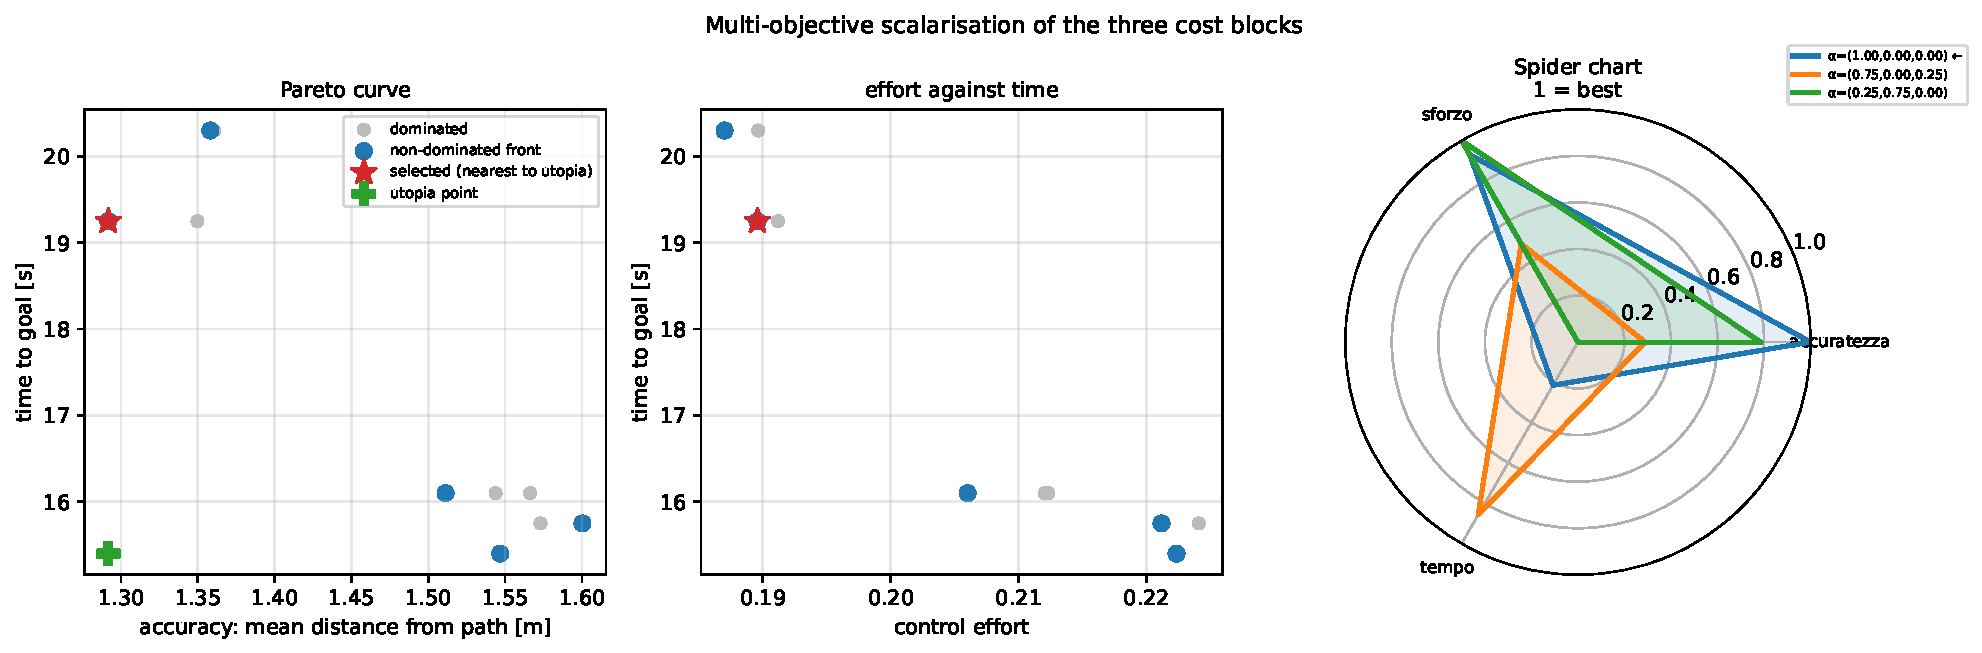
\includegraphics[width=\textwidth]{pareto_front}
  \caption{Sampling of the weight simplex: the achieved objectives for each scalarisation, the non-dominated
  set, and the utopia point. The metrics used to \emph{evaluate} the solutions use fixed weights, not the
  sampled ones --- otherwise each point of the simplex would be judged by a different yardstick.}
  \label{fig:pareto}
\end{figure}

Over $\resParetoPoints$ points of the simplex, $\resParetoNondom$ are non-dominated and the front is convex
(\resParetoConvex), so the weighted-sum scalarisation can in principle reach all of it --- a caution worth
verifying rather than assuming, since a non-convex front would leave part of itself unreachable by
\eqref{eq:scalar}.

The relative excursions say which objectives actually respond: accuracy moves by $\resParetoRelAcc\%$ across
the simplex, against $\resParetoRelEffort\%$ for effort and $\resParetoRelTime\%$ for time. Only accuracy is
genuinely under the control of the weights. Time and effort are nearly fixed, and Section~\ref{sec:pathfollow}
explains why: in path-parametrised mode the solver saturates $v_{x,\max}$ almost everywhere, so the duration
of the mission is decided by the kinematics and the input bounds rather than by the tuning. The trade-off is
real but mild, and the practical conclusion is that weight tuning is not where this system is limited ---
unlike the control horizon, which Section~\ref{sec:nc} shows to be leaving a factor of two in solve time on
the table.

\subsection{Offline weight tuning by Bayesian optimization}
\label{sec:bo}

Section~\ref{sec:pareto} measured how far the weights can move the closed loop. This section states the
program that chooses them, which is the third optimization problem in the stack and the only one that is not
solved online.

The eleven weights of the cost~\eqref{eq:cost} and of the obstacle term~\eqref{eq:barrier},
\begin{equation}
  \theta=\big(Q_x,\,Q_y,\,Q_\psi,\,\rho_T,\,R_{v_x},\,R_{v_y},\,R_\omega,\,\Rjerk,\,\Wobs,\,\aobs,\,\robs\big)
  \in\Theta\subset\R^{11},
  \label{eq:theta}
\end{equation}
are the decision variables of a second-level problem
\begin{equation}
  \hat\theta \;=\; \arg\min_{\theta\in\Theta}\;\mathcal{J}(\theta),
  \label{eq:outer}
\end{equation}
where $\mathcal{J}$ measures closed-loop navigation quality. Problem~\eqref{eq:outer} shares none of the
structure that Sections~\ref{sec:dims} and~\ref{sec:deriv} exploit: $\mathcal{J}$ has no closed form, no
derivatives, and one evaluation costs a full navigation rollout. It is a black-box problem, and the standard
tool is a Gaussian-process surrogate \cite{rasmussen2006gp,shahriari2016bo}.

The obstacle is dimension, and it is worth being precise about it because it dictates the method. A surrogate
over $\Theta\subset\R^{11}$ needs a sample density that a rollout-priced objective cannot supply: a budget of
$n$ evaluations covers each axis with $n^{1/11}$ points, so even a hundred rollouts amount to fewer than two
points per coordinate. A surrogate fitted on such a sample spends most of its capacity on coordinates that
turn out not to matter, and any acquisition rule that rewards unexplored regions never runs out of them.

\paragraph{The objective.} Each evaluation is a full closed-loop mission driving the production tracker, with
a time cap:
\begin{equation}
  \mathcal{J}(\theta)=
  \begin{cases}
    T_{\mathrm{goal}}/T_{\mathrm{ref}}, & \text{goal reached},\\[2pt]
    10+5\,d_{\mathrm{final}}/d_0, & \text{otherwise},
  \end{cases}
  \;+\;c_u\,\overline{\|\Delta u\|}\;+\;c_t\,\bar t\;+\;c_d\max\big(0,\,\dsafe-d_{\min}\big),
  \label{eq:Jcl}
\end{equation}
with $T_{\mathrm{ref}}=d_0/v_{\mathrm{ref}}$ the time a straight run at cruise speed would take,
$d_{\mathrm{final}}$ the residual distance to the goal, $\overline{\|\Delta u\|}$ the mean input increment,
$\bar t$ the mean solve time and $d_{\min}$ the minimum clearance. The branch structure is the part that
matters. A configuration that does not complete the mission is scored on the \emph{fraction of the distance
it closed}, so the objective stays informative on failures instead of saturating at a constant penalty; and
because~\eqref{eq:Jcl} is evaluated in closed loop rather than on a recorded trajectory, it can observe a
deadlock, which is a failure mode no one-step prediction score can see.

\paragraph{Per-axis surrogates and coordinate descent.} Rather than one surrogate over $\R^{11}$, the scheme
fits \emph{eleven one-dimensional} Gaussian processes, one per coordinate. Writing
$\theta=(\theta_i,\theta_{-i})$, each axis is explored on a uniform design of $m$ values spanning its
interval while $\theta_{-i}$ is held fixed, and a $1$-D GP with a Mat\'ern-$5/2$ kernel and a white-noise
term,
\begin{equation}
  k(\theta_i,\theta_i')=\sigma_f^2\Big(1+\sqrt5\,\tfrac{|\theta_i-\theta_i'|}{\ell}
  +\tfrac53\tfrac{(\theta_i-\theta_i')^2}{\ell^2}\Big)e^{-\sqrt5|\theta_i-\theta_i'|/\ell}
  +\sigma_n^2\delta(\theta_i,\theta_i'),
  \label{eq:kernel}
\end{equation}
is fitted to those observations by maximising the log marginal likelihood. The axis optimum is the minimiser
of the posterior \emph{mean} over a fine grid,
\begin{equation}
  \hat\theta_i \;=\; \arg\min_{\theta_i\in[\ell_i,u_i]}\; \mu_i(\theta_i),
  \label{eq:axisopt}
\end{equation}
which uses the smoothed estimate rather than the best sampled point and therefore does not require the
optimum to fall on a grid node. The total cost is $11m+1$ rollouts, and the by-product is worth as much as
the optimum: eleven curves with error bands, each showing how much the objective actually depends on the
weight in question, on which the reader can check the tuning instead of trusting it.

Three decisions make the scheme defensible, and each is a place where it could quietly go wrong.
\emph{Separability.} Assembling per-axis optima into one vector is exact only when
$\mathcal{J}(\theta)\approx\sum_i f_i(\theta_i)$, which is not true here: the barrier height and the safety
radius interact, since a tall barrier is harmless when its radius is small. The assumption is therefore
repaired by the next decision and verified a posteriori by evaluating the assembled vector.
\emph{Sequential update and ordering.} The axes are swept in decreasing order of influence and each optimum
is fixed before the next axis is visited, so later sweeps are conducted about an already improved operating
point. This is coordinate descent with a GP line search, and it is what makes the scheme robust to the
interactions separability ignores: sweeping the dominant coordinate first moves the base point out of the
region where the mission fails, so every subsequent sweep is measured where the objective discriminates.
\emph{Significance floor.} A $1$-D GP fitted to a handful of points returns an optimum on any axis, including
one on which the objective does not move. An axis is accepted only if the spread of its observations exceeds
the run-to-run scatter; otherwise the weight keeps its default. Without that floor the procedure reports
eleven confident optima and several of them are noise.

\paragraph{What this can be expected to buy.} The scalarisation sweep of Section~\ref{sec:pareto} already
bounds the answer, and the bound is the reason to read the two sections together. Across the whole weight
simplex the tracking accuracy moves by $\resParetoRelAcc\%$ while the time to goal moves by
$\resParetoRelTime\%$ and the control effort by $\resParetoRelEffort\%$: on a mission the robot completes,
the weights control how closely it follows the path and very little else, because the duration is set by the
input bounds and not by the tuning. A tuning procedure can therefore be expected to buy accuracy and
smoothness, and any large gain it reports must come from the failure branch of~\eqref{eq:Jcl} --- from
configurations that do not reach the goal at all --- rather than from trimming one that already works. That
is a useful prediction to hold in advance of the campaign, because it says which number to distrust.

The campaign itself has not yet been run on the deployed profile. It is priced in rollouts, and re-running it
before the kinematics and the two horizons are settled would tune a configuration that is about to change;
the procedure above is stated here so that the measurement, when it is made, is read against a prediction
rather than on its own.

\subsection{Non-convex obstacles, and the target rule that fails on them}
\label{sec:nonconvex}

\subsubsection{The limit cycle}
\label{sec:localmin}

The clearest illustration in this study of the difference between solving an optimization problem well and
posing the right one does not involve the NLP at all. With the projection rule~\eqref{eq:localgoal} the
stack livelocks in front of a non-convex obstacle. The ray to the goal enters the concavity, so the local
target lands inside it; \astar{} correctly routes around the obstacle \emph{inside the window} and the MPC
tracks that path faithfully; the robot leaves; and the moment it is out, the ray points back in. Every NLP in
that run is solved to optimality, and every one of them answers a question that should not have been asked.

The failure is not a coincidence of geometry, and this is the point that took the longest to see. It is
\emph{deterministic}: the ray from the robot to the goal points into the concavity for as long as the robot
is in front of it, whatever the map contains. Adding memory of the \emph{obstacles} therefore does not repair
it --- the robot may have mapped every cell of the wall and will still aim past it --- because the defect is
in how the target is chosen, not in what is remembered about the world. The diagnostic that settles it is the
one in Section~\ref{sec:astar}: standing inside a dead end, the boundary cells that lead out and the boundary
cells that lead further in are at almost the same Euclidean distance from the goal, so the rule declares them
equivalent and picks between them arbitrarily, changing its mind at every replanning cycle. Under the
geodesic distance on the free space already observed, the same cells differ by an order of magnitude.

Three structural facts conspire, and all three are properties of the \emph{formulation} rather than of the
tuning. The target rule is a projection and not a decision, in the sense made precise
by~\eqref{eq:localgoalargmin}. The occupancy grid is volatile, so nothing survives one grid width of travel
unless it is stored deliberately. And the input set of~\eqref{eq:cons-vx} makes backing out of a pocket
expensive: reversing is admitted but bounded well below the forward speed, so the cheap escape is a wide
forward arc, which is exactly the manoeuvre a concavity denies. The repair must live in the target rule,
which is where the failure lives.

\subsubsection{The two repairs, and what each of them fixes}
\label{sec:memoryfix}

Equation~\eqref{eq:localgoalargmin} has two ingredients that the projection rule~\eqref{eq:localgoal} does
not use at all, and they were expected to repair different halves of the failure.

\paragraph{The metric: a geodesic field.} Replacing the Euclidean $d_k$ with the geodesic distance to the
goal over the free cells of the accumulated map costs one scalar field per replanning cycle --- a wavefront
propagated from the goal, with no path extracted --- and it is what makes the rule use the evidence the robot
has already collected. Unobserved space is treated as free, which is the optimistic assumption of frontier
exploration, and the consequence is intended: while the far end of a corridor is unknown the field runs
through it and entering is the correct decision, and the moment the end is observed the same target becomes
distant and is discarded. The field corrects itself as the sensor discovers, rather than committing on the
strength of what has not been seen.

\paragraph{The memory: a tabu tied to progress.} The second ingredient penalises cells already visited
without progress. Its erasure rule is the part that carries the argument: a tabu that decays on a clock does
not remove the limit cycle, it lengthens its period, because the moment the penalty fades the ray points back
into the trap. The penalty is therefore released by \emph{progress} --- by the best distance to the goal ever
achieved improving --- and not by time. Note also why the tabu cannot be folded into the edge cost
of~\eqref{eq:astarcost}: a cell cost changes the \emph{path} towards a fixed target, not the \emph{choice} of
target, so making the dead end expensive merely makes traversing it expensive. The lever is the target.

\paragraph{Memory that survives noise.} Both repairs read the same accumulated map, and its construction has
to tolerate a sensor that lies occasionally. Every return is quantised to its cell in the \emph{world} frame
and stored with the time it was last seen and the number of \emph{distinct scans} in which it has appeared; a
cell is \emph{confirmed} once that count reaches two. A wall is re-hit by every scan that ranges it, while a
spurious return lands in its cell exactly once and never becomes an obstacle. Contradicting evidence is
allowed to win as well: every beam passing \emph{through} a remembered cell on its way to a farther return
deletes it, stopping short of the endpoint so that a ray never carves the surface it terminates on. A real
wall cannot be carved, because beams end on it; a phantom cell standing in an open passage is crossed, and
erased, by every scan that ranges through it.

\paragraph{Three hardening rules, each found by watching its absence fail.} Confirmed cells are
\emph{removed from the search graph}, not merely inflated: under the soft cost~\eqref{eq:astarcost} a
remembered wall is only a finite obstacle, and an early version dutifully tunnelled through it the moment the
detour became more expensive than the wall. Inflation prices \emph{proximity}, memory records
\emph{evidence}, and only the latter may veto an edge. One-cell pinholes among confirmed cells are sealed in
the routing graph, because at sensor range the beam spacing exceeds the cell size and a remembered wall
carries single-cell gaps that open and close as scans accumulate --- each a phantom shortcut that flips the
global route. And the local execution graph dilates confirmed cells by the robot radius, so that no executed
path passes within a body radius of known structure. The two graphs are deliberately not treated alike:
dilating the routing graph makes the committed route invalidate itself as the observed wall grows under the
robot's own approach, while sealing the execution graph after dilation counts the body twice and closes every
doorway the robot actually fits through. Stability lives in the routing graph, clearance in the execution
graph.

\paragraph{The measurement.} The closed-loop comparison of the three rules --- the baseline projection, the
geodesic metric and the tabu --- has now been run over four worlds under the limited-perception model of
Section~\ref{sec:setup}, with the production planner and a $300$~s budget per run. Table~\ref{tab:escape}
reports it. The prediction stated above is confirmed on the first two counts and refuted on the third.

\begin{table}[htbp]
  \centering
  \small
  \caption{Escape from non-convex obstacles under limited perception: the baseline Euclidean projection
  against the deployed geodesic metric, each with and without the tabu. Time is capped at $300$~s; a run that reaches
  the cap did not reach the goal. \emph{Crossing} marks a run that reached the goal by passing through an
  obstacle --- the harness plant has no collision response, so a reached goal must always be read together
  with the clearance.}
  \label{tab:escape}
  \begin{tabular}{llcrrr}
    \toprule
    World & Target rule & Goal & Time [s] & Path [m] & Clearance [m] \\
    \midrule
    \texttt{long\_wall}  & Euclidean          & \emph{crossing} & 71.4 & 28.9 & 0.027 \\
                         & geodesic           & yes & 62.3 & 25.4 & 0.896 \\
    \midrule
    \texttt{horseshoe}   & Euclidean          & no  & --- & 93.4 & 1.919 \\
                         & geodesic           & yes & 100.4 & 38.5 & 0.853 \\
    \midrule
    \texttt{dead\_end}   & Euclidean          & no  & --- & 79.4 & 0.659 \\
                         & geodesic           & yes & 81.6 & 31.7 & 0.669 \\
    \midrule
    \texttt{l\_corridor} & Euclidean          & no  & --- & 79.7 & 0.801 \\
                         & geodesic           & yes & 112.7 & 41.8 & 0.801 \\
    \bottomrule
  \end{tabular}
\end{table}

The projection rule fails on every world. On \texttt{horseshoe}, \texttt{dead\_end} and \texttt{l\_corridor} it
exhausts the budget without reaching the goal, and the signature is the one the analysis predicts: $117$,
$140$ and $137$ direction reversals respectively, over paths of $79$ to $93$~m that never leave the mouth of
the obstacle --- the furthest the robot ever gets is $2.4$ to $4.6$~m along the axis to the goal. That is a
limit cycle, measured, not a slow traversal. On \texttt{long\_wall} it reports the goal reached, and the
clearance column says why that must not be counted: $0.027$~m, i.e.\ it went through the wall. The harness
plant integrates the model without collision response, so a target rule that aims into an obstacle produces a
trajectory that passes through it, and only the clearance exposes the difference.

The geodesic metric alone resolves all four, with clearances between $0.669$ and $0.896$~m --- well clear of
the $0.35$~m body radius --- and with the reversal count collapsing from over a hundred to between two and
eight. On \texttt{horseshoe} and \texttt{dead\_end} the escape takes two reversals: the robot enters, observes
the closing wall, and leaves. This is the intended behaviour of an optimistic field that corrects itself as
the sensor discovers, and it is the direct measurement of the argument made above.

The third count is where the prediction fails. The tabu changes nothing: with the geodesic metric the runs
are identical to the last decimal on every world, and without it the tabu does not rescue a single failure.
The reason is visible once stated. The tabu penalises cells already visited, but the candidate targets are on
the frontier of the known region, which by construction has not been visited --- so the penalty evaluates to
zero on precisely the cells the rule is choosing between. The mechanism was never able to act. It is retained
in the code, disabled, and the honest conclusion is that the metric was the whole repair and the memory was a
hypothesis the data does not support.

\subsection{Summary of design guidelines}
\label{sec:guidelines}

Table~\ref{tab:guidelines} collects the actionable outcome of the campaigns above. Each row names the
deployed choice, the choice the measurement supports, and where the evidence is.

\begin{table}[htbp]
  \centering
  \small
  \caption{Design guidelines extracted from the numerical study. Bold in the second column marks a
  recommendation that differs from what is deployed.}
  \label{tab:guidelines}
  \begin{tabular}{p{0.21\textwidth}p{0.19\textwidth}p{0.52\textwidth}}
    \toprule
    Decision & Deployed / supported & Evidence \\
    \midrule
    Integration scheme & mid-point / keep & Order $\resOrderMidpoint$ against $\resOrderEuler$,
      $\resIntegratorGain\times$ more accurate for one addition (\S\ref{sec:discretization}) --- but see the
      next row before spending anything more here. \\
    Prediction model & lag model / \textbf{revisit} & Divergence $\resPredDivergence$~m per horizon,
      $\resPredVsMidpoint\times$ the integrator error: the model, not the arithmetic, is the dominant term
      (\S\ref{sec:prederr}). \\
    Parametrisation & multiple shooting / keep & Hessian $\resShootHessDensMulti\%$ dense against
      $\resShootHessDensSingle\%$ condensed; claim the structure, not the speed (\S\ref{sec:shoot}). \\
    Obstacle relaxation & smooth penalty / keep, with $\ell^1$ available & $\ell^1$ slack exactly zero from
      $\rho_s=\resRhoLoneZero>\mu^\star$; $\ell^2$ never vanishes (\S\ref{sec:l1}). \\
    Obstacle at $k=0$ & excluded / keep & Including it cannot change the solution and makes the program
      infeasible exactly when it matters (\S\ref{sec:statement}, \S\ref{sec:l1}). \\
    Terminal ingredient & none / \textbf{add} & Slack identically zero, cost $\resTermCostMin\%$ to
      $\resTermCostMax\%$; but the result is flattered by the degenerate lag and must be re-measured under
      physics (\S\ref{sec:terminal}). \\
    Reference & time-parametrised / \textbf{path-parametrised} & $+\resAdvanceGain\%$ advance per horizon and
      one parameter eliminated, at $+70\%$ iterations (\S\ref{sec:pathfollow}). \\
    Derivatives & AD / keep & $\resADratio$ objective evaluations against $\resFDcentralEvals$, and more
      accurate; finite differences would cost $\resFDcentralBudget\%$ of the cycle budget
      (\S\ref{sec:deriv}). \\
    Hessian & exact / keep & $\resIterExactHess$ against $\resIterLBFGS$ iterations
      ($-\resHessIterSaving\%$) at the same optimum (\S\ref{sec:deriv}). \\
    Solver class & interior point / keep & $\resSolverRatioLow\times$ faster at $\resSolverIneqLow$
      inequalities, $\resSolverRatioHigh\times$ at $\resSolverIneqHigh$ (\S\ref{sec:solvercmp}). \\
    Barrier weight $\Wobs$ & $\resWobsDep$ / keep & Below the bifurcation threshold
      $[\resBifLow,\resBifHigh]$: the control law is regular in $x_0$ (\S\ref{sec:bif}). \\
    Horizon $N,\Delta t$ & $\resN$, $\resDt$~s / \textbf{$N=26$, $\Delta t=0.35$~s} & Dominated, but only
      marginally on $(N,\Delta t)$ alone; the real gain needs $\Ninput$ (next row). Short horizons win on
      time and lose on safety: every configuration with $N\Delta t\le2$~s grazes (\S\ref{sec:horizon}). \\
    Control horizon $\Ninput$ & $=N$ / \textbf{$\Ninput=10$} & With $N=26$: same time to goal, same
      clearance, tail solve time $24.3$~ms against $59.3$ (\S\ref{sec:nc}). \\
    Move blocking & absent / \textbf{add} & Earlier defended as a considered choice; the joint sweep
      withdraws both grounds, and the recorded run misses its cycle budget ($157.9$~ms against
      $\resCycleBudget$) (\S\ref{sec:nc}). \\
    Weight tuning & scalarisation / not critical & Only accuracy responds ($\resParetoRelAcc\%$ against
      $\resParetoRelTime\%$ on time): not where the system is limited (\S\ref{sec:pareto}). The per-axis
      Bayesian procedure of \S\ref{sec:bo} is stated, and bounded in advance by that result, but not yet
      run on this profile. \\
    Input envelope & narrow / \textbf{as wide as the policy allows} & Critical cone contracts to
      $\resConeLast$; the tightened constraint and the $\ell^1$ constraint fail on $\mathcal{U}$, not on
      the data (\S\ref{sec:kkt}, \S\ref{sec:l1}, \S\ref{sec:robust}). The envelope has since been
      widened to $v_{y,\max}=\resVyMax$ against $v_{x,\max}=\resVxMax$, which is the recommendation acted
      on; the three measurements above predate it. \\
    Local-target metric & Euclidean / \textbf{geodesic} & The rule~\eqref{eq:localgoal} rates the boundary
      cells that lead out of a dead end and those that lead further in as equivalent. Measured over four
      non-convex worlds: the Euclidean rule fails all four, the geodesic resolves all four
      (Table~\ref{tab:escape}, \S\ref{sec:nonconvex}). \\
    Target memory & none / keep none & The tabu was predicted to be needed and measured not to be: with the
      geodesic metric the runs are identical with and without it, because the candidate targets lie on the
      unvisited frontier where the penalty is identically zero (\S\ref{sec:memoryfix}). \\
    \bottomrule
  \end{tabular}
\end{table}

%=============================================================================
\section{Discussion and limitations}
\label{sec:discussion}

\paragraph{What the formulation guarantees, and what it does not.} In its deployed configuration the NLP is
always feasible, because the only constraints are the dynamics and the input box; for a real-time loop with
no fallback trajectory this is a genuine robustness property, and it is why the penalty formulation was
preferred to a constrained one. But there is no terminal set in that configuration and no Lyapunov argument,
so nominal asymptotic stability and recursive feasibility in the standard sense
\cite{mayne2000constrained} are not established. Section~\ref{sec:terminal} supplies the missing ingredient
and prices it, and Section~\ref{sec:l1} supplies the exact relaxation that makes a constrained formulation
survivable; assembling the two into a configuration that is simultaneously deployable and certified is the
natural next step, and it is now cheaper than this report previously argued: Section~\ref{sec:nc} shows that
the long prediction horizon a rigorous terminal ingredient would want can be carried at \emph{lower} solve
cost than the present short one, by blocking the inputs rather than shortening the prediction. What such a
configuration would still have to prove is that the terminal set remains reachable once the actuator lag is
identified under physics, where the degenerate lag of Section~\ref{sec:terminal} no longer flatters it.

\paragraph{The weakest link is not the optimizer.} Every campaign in Section~\ref{sec:performance} solved its
NLP successfully, and Section~\ref{sec:kkt} certifies those solutions as strict local minima with unique
multipliers. The systematic failures of the system are elsewhere. One is a \emph{modelling} failure: the
prediction diverges from the plant by $\resPredDivergence$~m over a single horizon, and no amount of
numerical care inside the program can repair a model that is a planar holonomic agent standing in for a
walking humanoid. The other is a \emph{formulation} failure: the greedy rolling-horizon target rule of
Section~\ref{sec:localmin} discards the topology of the free space, and the repair had to be posed in the
target rule rather than in the NLP.

\paragraph{The input set is the binding constraint, and it is not in the cost.} Three independent
measurements converge on this. The critical cone contracts to $\resConeLast$ dimensions
(\S\ref{sec:kkt}); the $\ell^1$-relaxed obstacle constraint was infeasible at demanding clearances because
lateral translation is bounded far below forward travel (\S\ref{sec:l1}, where the widening of the envelope
now puts that finding up for re-measurement); and the constraint tightening is inert on the recorded run for
the same reason (\S\ref{sec:robust}). A controller whose admissible set has
been reduced to essentially one degree of freedom is not being limited by its objective, and effort spent on
weights is effort spent on the wrong object.

\paragraph{Scope of the numbers, stated plainly.} The plant used throughout is kinematic, and deliberately
so: with the prediction model equal to the simulation model, the experiments measure the optimizer rather
than the gait. The price is that every conclusion depending on the actuator pole is out of reach here ---
which is why the selection of the sampling time from the plant bandwidth, a standard piece of this analysis,
is absent from this report and deferred until $\tau$ is identified under physics. Two further limits belong
in the same paragraph. The closed-loop counterfactuals use synthetic worlds, one of which (the U-trap) grazes
obstacles in every configuration and therefore cannot support any comparison of clearances. And the loop is
closed through a look-ahead setpoint rather than by applying $u^\star_0$, which washes out fine differences
between MPC solutions and is why the constraint tightening of Section~\ref{sec:robust} could be verified in
the plan but not in the executed trajectory.

%=============================================================================
\section{Conclusions}
\label{sec:conclusions}

This report analysed a deployed map-free navigation stack as what it is numerically: an exact \astar{} search
on a Gaussian occupancy grid, a $\resNvar$-variable nonlinear program with a $\resJacDensity\%$ dense
constraint Jacobian, and a set of design decisions each of which has a defensible alternative in the theory.

The decisions that survived measurement are worth stating as such. Algorithmic differentiation costs
$\resADratio$ objective evaluations against $\resFDcentralEvals$ for central differences and is exact, which
is what makes the exact Hessian affordable and buys $\resHessIterSaving\%$ of the iterations. The
interior-point method is faster than the active-set alternative in both regimes into which this problem can
be put, and its margin widens with the number of inequalities exactly as expected. The deployed obstacle
weight sits below the bifurcation threshold, so the control law is a regular function of the state. And the
first- and second-order optimality conditions hold at every cycle examined, with unique multipliers.

Four results contradicted the design, and they are the ones that taught the most. The mid-point rule is
$\resIntegratorGain\times$ more accurate than the scheme it replaced and changes the closed loop by
essentially nothing, because the prediction is limited by the model and not by its integration. The deployed
horizon is dominated: a configuration a quarter of the size matches it on task performance at a third of the
tail solve time. Making the path abscissa a decision variable buys $\resAdvanceGain\%$ more progress per
horizon and removes a hand-set parameter rather than replacing it with another. And the constraint that
decides what the controller can do is not in the cost at all: with the lateral bound at $\resVyMax$~m/s and
reversing bounded well below forward travel, the critical cone contracts to $\resConeLast$ dimensions and
the controller ends the
mission executing the only motion still admissible.

The natural continuations follow directly. Identify the actuator time constant under physics, which unblocks
both the sampling-time analysis and an honest re-measurement of the terminal constraint. Apply $u^\star_0$
directly instead of through a look-ahead setpoint, so that improvements provable in the plan become
observable in the trajectory. Adopt the path-parametrised reference, whose cost is known and whose benefit is
measured. And revisit the input envelope before the cost weights, because that is where the evidence points.

%=============================================================================
\section*{Reproducibility}
\addcontentsline{toc}{section}{Reproducibility}

Every number, table and figure in this report is generated from the deployed code by a single command and
enters the document through macros and included files, not by transcription. The measurements were taken on
commit \texttt{\resCommit} of branch \texttt{\resBranch} (\resDate), with the profile \resProfile{}, the
recorded run \resBag, CasADi~\resCasadi{} and NumPy~\resNumpy. The generator verifies the LaTeX it produces
before writing it --- balanced environments, table rows matching their column specification, mathematical
tokens inside math mode, macros used in the text but never defined, and cross-references without a target ---
and it refuses to emit a document that fails any of those checks. Assertions in the text are conditioned on
the data: where a fitted exponent does not reach its predicted value, where a Pareto front is not
informative, or where a sweep contains no case that exhibits the effect under discussion, the generated text
says so instead of reporting the expected conclusion. Re-running the campaign and recompiling updates the
report; a parameter changed in the code and not in the text cannot go unnoticed, because there is no text to
change.

%=============================================================================
\bibliography{bibliography}

\end{document}
